%-------------------------------------------------------------------------------
% This file provides a skeleton ATLAS paper.
%-------------------------------------------------------------------------------
% \pdfoutput=1
% The \pdfoutput command is needed by arXiv/JHEP/JINST to ensure use of pdflatex.
% It should be included in the first 5 lines of the file.
% \pdfinclusioncopyfonts=1
% This command may be needed in order to get \ell in PDF plots to appear. Found in
% https://tex.stackexchange.com/questions/322010/pdflatex-glyph-undefined-symbols-disappear-from-included-pdf
%-------------------------------------------------------------------------------
% Specify where ATLAS LaTeX style files can be found.
\newcommand*{\ATLASLATEXPATH}{latex/}
% Use this variant if the files are in a central location, e.g. $HOME/texmf.
% \newcommand*{\ATLASLATEXPATH}{}
%-------------------------------------------------------------------------------
\documentclass[PAPER, atlasdraft=true, texlive=2016, UKenglish]{\ATLASLATEXPATH atlasdoc}
% The language of the document must be set: usually UKenglish or USenglish.
% british and american also work!
% Commonly used options:
%  atlasdraft=true|false This document is an ATLAS draft.
%  texlive=YYYY          Specify TeX Live version (2016 is default).
%  coverpage             Create ATLAS draft cover page for collaboration circulation.
%                        See atlas-draft-cover.tex for a list of variables that should be defined.
%  cernpreprint          Create front page for a CERN preprint.
%                        See atlas-preprint-cover.tex for a list of variables that should be defined.
%  NOTE                  The document is an ATLAS note (draft).
%  PAPER                 The document is an ATLAS paper (draft).
%  CONF                  The document is a CONF note (draft).
%  PUB                   The document is a PUB note (draft).
%  BOOK                  The document is of book form, like an LOI or TDR (draft)
%  txfonts=true|false    Use txfonts rather than the default newtx
%  paper=a4|letter       Set paper size to A4 (default) or letter.

%-------------------------------------------------------------------------------
% Extra packages:
\usepackage{\ATLASLATEXPATH atlaspackage}
% Commonly used options:
%  biblatex=true|false   Use biblatex (default) or bibtex for the bibliography.
%  backend=bibtex        Use the bibtex backend rather than biber.
%  subfigure|subfig|subcaption  to use one of these packages for figures in figures.
%  minimal               Minimal set of packages.
%  default               Standard set of packages.
%  full                  Full set of packages.
%-------------------------------------------------------------------------------
% Style file with biblatex options for ATLAS documents.
\usepackage{\ATLASLATEXPATH atlasbiblatex}

% Useful macros
\usepackage{\ATLASLATEXPATH atlasphysics}
% See doc/atlas_physics.pdf for a list of the defined symbols.
% Default options are:
%   true:  journal, misc, particle, unit, xref
%   false: BSM, heppparticle, hepprocess, hion, jetetmiss, math, process, other, texmf
% See the package for details on the options.

% Files with references for use with biblatex.
% Note that biber gives an error if it finds empty bib files.
% \addbibresource{.bib}
\addbibresource{bib/ATLAS.bib}
\addbibresource{bib/CMS.bib}
\addbibresource{bib/ConfNotes.bib}
\addbibresource{bib/PubNotes.bib}

% Paths for figures - do not forget the / at the end of the directory name.
\graphicspath{{logos/}{figures/}}

% Add you own definitions here (file ANA-TOPQ-2017-07-PAPER-defs.sty).
\usepackage{ANA-TOPQ-2017-07-PAPER-defs}

%-------------------------------------------------------------------------------
% Generic document information
%-------------------------------------------------------------------------------

% Title, abstract and document
%-------------------------------------------------------------------------------
% This file contains the title, author and abstract.
% It also contains all relevant document numbers used by the different cover pages.
%-------------------------------------------------------------------------------

% Title
%\AtlasTitle{Search for flavor-changing neutral current $t\rightarrow Hq$ ($q=u,c$) decays in pp collisions at $\sqrt{s}$=13 TeV with the ATLAS detector }
\AtlasTitle{Search for top quark decays $t \to Hq$ with 36 fb$^{-1}$ of $pp$ collision data at $\sqrt{s}=13~\tev$ with the ATLAS detector}

% Draft version:
% Should be 1.0 for the first circulation, and 2.0 for the second circulation.
% If given, adds draft version on front page, a 'DRAFT' box on top of each other page, 
% and line numbers.
% Comment or remove in final version.
\AtlasVersion{1.3}
% Abstract - % directly after { is important for correct indentation
\AtlasAbstract{%
A search for flavour-changing neutral current decays of a top quark into an up-type quark ($q=u, c$) and the 
Standard Model Higgs boson, $t\to Hq$, is presented. 
The search is based on a dataset of $pp$ collisions at $\sqrt{s}=13~\tev$ recorded in 2015 and 2016 with the ATLAS detector at the 
CERN Large Hadron Collider and corresponds to an integrated luminosity of 36.1 fb$^{-1}$.
Two complementary analyses are performed that search for top-quark pair events in which one top quark decays into $Wb$ and the other top quark decays into $Hq$,
and target the $H \to b\bar{b}$ and $H \to \tau^+\tau^-$ decay modes, respectively.  
The high multiplicity of $b$-quark jets, or the presence of hadronically decaying tau leptons, are exploited in the two analyses respectively. 
Multivariate techniques are used to separate the signal from the background, which is dominated by top-quark pair production.
No significant excess of events above the background expectation is found, and 95\% CL upper limits on the $t\to Hq$ branching ratios are derived.
The combination of these searches with ATLAS searches in diphoton and multilepton final states 
%significantly improves the sensitivity, 
yields observed (expected) 95\% CL upper limits on the $t\to Hc$ and $t\to Hu$ branching ratios of $1.1 \times 10^{-3}$ ($8.3 \times 10^{-4}$) 
and $1.2 \times 10^{-3}$ ($8.3 \times 10^{-4}$), respectively.
The corresponding combined observed (expected) upper limits on the $|\lambda_{tcH}|$ and $|\lambda_{tuH}|$ couplings are 0.064 (0.055) and 0.066 (0.055) respectively. 
These are the most restrictive direct bounds on $tqH$ interactions measured so far.
}

% Author - this does not work with revtex (add it after \begin{document})
\author{The ATLAS Collaboration}

% ATLAS reference code, to help ATLAS members to locate the paper
%\AtlasRefCode{TOPQ-2017-07}
%\AtlasRefCode{ATLAS-CONF-2018-049}

% ATLAS date - arXiv submission; usually filled in by the Physics Office
% \AtlasDate{\today}

% ATLAS heading - heading at top of title page. Set for TDR etc.
%\AtlasHeading{ATLAS ABC TDR}

% Submission journal and final reference
\AtlasJournal{JHEP}
% \AtlasJournal{Phys.\ Lett.\ B.}
% \AtlasJournalRef{\PLB 789 (2017) 123}
% \AtlasDOI{}

 %-------------------------------------------------------------------------------
% The following information is needed for the cover page. The commands are only defined
% if you use the coverpage option in atlasdoc or use the atlascover package
%-------------------------------------------------------------------------------

% List of supporting notes  (leave as null \AtlasCoverSupportingNote{} if you want to skip this option)
\AtlasCoverSupportingNote{Search for $\ttbar \to WbHq$, $H \to b\bar{b}$}{https://cds.cern.ch/record/2257631}
\AtlasCoverSupportingNote{Search for $\ttbar \to WbHq$, $H \to \tau^+\tau^-$}{https://cds.cern.ch/record/2273683}
\AtlasCoverSupportingNote{Combination of $\ttbar \to WbHq$ searches}{https://cds.cern.ch/record/2312520/}
%
% OR (the 2nd option is deprecated, especially for CONF and PUB notes)
%
% Supporting material TWiki page  (leave as null \AtlasCoverTwikiURL{} if you want to skip this option)
% \AtlasCoverTwikiURL{https://twiki.cern.ch/twiki/bin/view/Atlas/WebHome}

% Comment deadline
\AtlasCoverCommentsDeadline{3 September 2018}

% Analysis team members - contact editors should no longer be specified
% as there is a generic email list name for the editors
\AtlasCoverAnalysisTeam{
$H \to b\bar{b}$: Trisha Farooque, Davide Gerbaudo, Aurelio Juste, Nicola Orlando,  \\ Cheng Peng,  Laura Pereira, 
Yulia Rodina, Yanjun Tu,  Lo\"ic Val\'ery, \\ Tal Van Daalen, Jia-Shian Wang, Daiki Yamaguchi; \\
$H \to \tau^+\tau^-$: Xin Chen, Antonio De Maria, Boyang Li, Ligang Xia, Gang Zhang; \\
Combination: Peter Onyisi, Harish Potti}

% Editorial Board Members - indicate the Chair by a (chair) after his/her name
% Give either all members at once (then they appear on one line), or separately
\AtlasCoverEdBoardMember{Ketevi Assamagan~(chair), Garabed Halladjian, Fabrice Hubaut, Michele Weber~(chair)}

% \AtlasCoverEdBoardMember{EdBoard~Chair~(chair)}
% \AtlasCoverEdBoardMember{EB~Member~1}
% \AtlasCoverEdBoardMember{EB~Member~2}
% \AtlasCoverEdBoardMember{EB~Member~3}

% Editors egroup
\AtlasCoverEgroupEditors{atlas-TOPQ-2017-07-editors@cern.ch}

% EdBoard egroup
\AtlasCoverEgroupEdBoard{atlas-TOPQ-2017-07-editorial-board@cern.ch}

 

% Author and title for the PDF file
\hypersetup{pdftitle={ATLAS document},pdfauthor={The ATLAS Collaboration}}

%-------------------------------------------------------------------------------
% Content
%-------------------------------------------------------------------------------
\begin{document}

\maketitle

\tableofcontents


%-------------------------------------------------------------------------------
\section{Introduction}
\label{sec:intro}
%-------------------------------------------------------------------------------

Place your introduction here.


%-------------------------------------------------------------------------------
\section{ATLAS detector}
\label{sec:detector}
%-------------------------------------------------------------------------------

The ATLAS detector~\cite{PERF-2007-01} ...
% % Footnote with ATLAS coordinate system
\newcommand{\AtlasCoordFootnote}{%
ATLAS uses a right-handed coordinate system with its origin at the nominal interaction point (IP)
in the centre of the detector and the $z$-axis along the beam pipe.
The $x$-axis points from the IP to the centre of the LHC ring,
and the $y$-axis points upwards.
Cylindrical coordinates $(r,\phi)$ are used in the transverse plane, 
$\phi$ being the azimuthal angle around the $z$-axis.
The pseudorapidity is defined in terms of the polar angle $\theta$ as $\eta = -\ln \tan(\theta/2)$.
Angular distance is measured in units of $\Delta R \equiv \sqrt{(\Delta\eta)^{2} + (\Delta\phi)^{2}}$.}

%-------------------------------------------------------------------------------
\subsection{Run 1 ATLAS detector example for a Letter}
\label{sec:atlas1}
%-------------------------------------------------------------------------------

The ATLAS experiment~\cite{PERF-2007-01} at the LHC is a multi-purpose particle detector
with a forward-backward symmetric cylindrical geometry and a near $4\pi$ coverage in 
solid angle.\footnote{\AtlasCoordFootnote}
It consists of an inner tracking detector surrounded by a thin superconducting solenoid
providing a \SI{2}{\tesla} axial magnetic field, electromagnetic and hadron calorimeters, and a muon spectrometer.
The inner tracking detector covers the pseudorapidity range $|\eta| < 2.5$.
It consists of silicon pixel, silicon micro-strip, and transition radiation tracking detectors.
Lead/liquid-argon (LAr) sampling calorimeters provide electromagnetic (EM) energy measurements
with high granularity.
A hadron (steel/scintillator-tile) calorimeter covers the central pseudorapidity range ($|\eta| < 1.7$).
The end-cap and forward regions are instrumented with LAr calorimeters
for both EM and hadronic energy measurements up to $|\eta| = 4.9$.
The muon spectrometer surrounds the calorimeters and is based on
three large air-core toroidal superconducting magnets with eight coils each.
The field integral of the toroids ranges between \num{2.0} and \SI{6.0}{\tesla\metre}
across most of the detector. 
The muon spectrometer includes a system of precision tracking chambers and fast detectors for triggering.
A three-level trigger system is used to select events.
The first-level trigger is implemented in hardware and uses a subset of the detector information
to reduce the accepted rate to at most \SI{75}{\kilo\hertz}.
This is followed by two software-based trigger levels that
together reduce the accepted event rate to \SI{400}{\hertz} on average
depending on the data-taking conditions during 2012.


%-------------------------------------------------------------------------------
\subsection{Run 1 ATLAS detector example for a paper making use of the whole detector}
\label{sec:atlas2}
%-------------------------------------------------------------------------------

The ATLAS detector~\cite{PERF-2007-01} at the LHC covers nearly the entire solid angle around the collision point.
It consists of an inner tracking detector surrounded by a thin superconducting solenoid, electromagnetic and hadronic calorimeters,
and a muon spectrometer incorporating three large superconducting toroidal magnets.
The inner-detector system (ID) is immersed in a \SI{2}{\tesla} axial magnetic field 
and provides charged particle tracking in the range $|\eta| < 2.5$.

The high-granularity silicon pixel detector covers the vertex region and typically provides three measurements per track, 
the first hit being normally in the innermost layer.
It is followed by the silicon microstrip tracker which usually provides four two-dimensional measurement points per track.
These silicon detectors are complemented by the transition radiation tracker,
which enables radially extended track reconstruction up to $|\eta| = 2.0$. 
The transition radiation tracker also provides electron identification information 
based on the fraction of hits (typically 30 in total) above a higher energy deposit threshold corresponding to transition radiation.

The calorimeter system covers the pseudorapidity range $|\eta| < 4.9$.
Within the region $|\eta|< 3.2$, electromagnetic calorimetry is provided by barrel and 
endcap high-granularity lead/liquid-argon (LAr) electromagnetic calorimeters,
with an additional thin LAr presampler covering $|\eta| < 1.8$,
to correct for energy loss in material upstream of the calorimeters.
Hadronic calorimetry is provided by the steel/scintillating-tile calorimeter,
segmented into three barrel structures within $|\eta| < 1.7$, and two copper/LAr hadronic endcap calorimeters.
The solid angle coverage is completed with forward copper/LAr and tungsten/LAr calorimeter modules
optimised for electromagnetic and hadronic measurements respectively.

The muon spectrometer (MS) comprises separate trigger and
high-precision tracking chambers measuring the deflection of muons in a magnetic field generated by superconducting air-core toroids.
The field integral of the toroids ranges between \num{2.0} and \SI{6.0}{\tesla\metre}
across most of the detector. 
A set of precision chambers covers the region $|\eta| < 2.7$ with three layers of monitored drift tubes,
complemented by cathode strip chambers in the forward region, where the background is highest.
The muon trigger system covers the range $|\eta| < 2.4$ with resistive plate chambers in the barrel, and thin gap chambers in the endcap regions.
A three-level trigger system is used to select interesting events~\cite{PERF-2011-02}.
The Level-1 trigger is implemented in hardware and uses a subset of detector information
to reduce the event rate to a design value of at most \SI{75}{\kHz}.
This is followed by two software-based trigger levels which together reduce the event rate to about \SI{200}{\Hz}.




%-------------------------------------------------------------------------------
\section{Analysis}
\label{sec:analysis}
%-------------------------------------------------------------------------------

You can find some text snippets that can be used in papers in \texttt{template/atlas-snippets.tex}.
Some of the snippets need the \texttt{jetetmiss} option passed to \texttt{atlasphysics}.
%\subsection{\Antikt}

The \antikt algorithm with a radius parameter of $R=0.4$ is used to reconstruct jets with a four-momentum recombination scheme, using \topos as inputs. Jet energy is calibrated to the hadronic scale with the effect of \pileup removed

\subsection{\Topos}

Hadronic jets are reconstructed from calibrated three-dimensional \topos.
Clusters are constructed from calorimeter cells that are grouped together using a topological clustering algorithm.
These objects provide a three-dimensional representation of energy depositions in the calorimeter and implement a nearest-neighbour noise suppression algorithm.
The resulting \topos are classified as either electromagnetic or hadronic based on their shape, depth and energy density.
Energy corrections are then applied to the clusters in order to calibrate them to the appropriate energy scale for their classification.
These corrections are collectively referred to as \textit{local cluster weighting}, or LCW, and jets that are calibrated using this procedure are referred to as LCW jets~\cite{PERF-2012-01}.

\subsection{Grooming}

Trimming removes subjets with $\ptsubji/\ptjet < \fcut$, where \ptsubji is the transverse momentum of the $i^{\text{th}}$ subjet, and $\fcut=0.05$.
Filtering proceeds similarly, but utilises the relative masses of the subjets defined and the original jet. For at least one of the configurations tested, trimming and filtering are both able to approximately eliminate the \pileup dependence of the jet mass.


%-------------------------------------------------------------------------------
\section{Results}
\label{sec:result}
%-------------------------------------------------------------------------------

Place your results here.

% All figures and tables should appear before the summary and conclusion.
% The package placeins provides the macro \FloatBarrier to achieve this.
% \FloatBarrier


%-------------------------------------------------------------------------------
\section{Conclusion}
\label{sec:conclusion}
%-------------------------------------------------------------------------------

Place your conclusion here.


%-------------------------------------------------------------------------------
\section*{Acknowledgements}
%-------------------------------------------------------------------------------

%% Acknowledgements for papers with collision data
% Version 24-Oct-2018

% Standard acknowledgements start here
%----------------------------------------------
We thank CERN for the very successful operation of the LHC, as well as the
support staff from our institutions without whom ATLAS could not be
operated efficiently.

We acknowledge the support of ANPCyT, Argentina; YerPhI, Armenia; ARC, Australia; BMWFW and FWF, Austria; ANAS, Azerbaijan; SSTC, Belarus; CNPq and FAPESP, Brazil; NSERC, NRC and CFI, Canada; CERN; CONICYT, Chile; CAS, MOST and NSFC, China; COLCIENCIAS, Colombia; MSMT CR, MPO CR and VSC CR, Czech Republic; DNRF and DNSRC, Denmark; IN2P3-CNRS, CEA-DRF/IRFU, France; SRNSFG, Georgia; BMBF, HGF, and MPG, Germany; GSRT, Greece; RGC, Hong Kong SAR, China; ISF and Benoziyo Center, Israel; INFN, Italy; MEXT and JSPS, Japan; CNRST, Morocco; NWO, Netherlands; RCN, Norway; MNiSW and NCN, Poland; FCT, Portugal; MNE/IFA, Romania; MES of Russia and NRC KI, Russian Federation; JINR; MESTD, Serbia; MSSR, Slovakia; ARRS and MIZ\v{S}, Slovenia; DST/NRF, South Africa; MINECO, Spain; SRC and Wallenberg Foundation, Sweden; SERI, SNSF and Cantons of Bern and Geneva, Switzerland; MOST, Taiwan; TAEK, Turkey; STFC, United Kingdom; DOE and NSF, United States of America. In addition, individual groups and members have received support from BCKDF, CANARIE, CRC and Compute Canada, Canada; COST, ERC, ERDF, Horizon 2020, and Marie Sk{\l}odowska-Curie Actions, European Union; Investissements d' Avenir Labex and Idex, ANR, France; DFG and AvH Foundation, Germany; Herakleitos, Thales and Aristeia programmes co-financed by EU-ESF and the Greek NSRF, Greece; BSF-NSF and GIF, Israel; CERCA Programme Generalitat de Catalunya, Spain; The Royal Society and Leverhulme Trust, United Kingdom. 

The crucial computing support from all WLCG partners is acknowledged gratefully, in particular from CERN, the ATLAS Tier-1 facilities at TRIUMF (Canada), NDGF (Denmark, Norway, Sweden), CC-IN2P3 (France), KIT/GridKA (Germany), INFN-CNAF (Italy), NL-T1 (Netherlands), PIC (Spain), ASGC (Taiwan), RAL (UK) and BNL (USA), the Tier-2 facilities worldwide and large non-WLCG resource providers. Major contributors of computing resources are listed in Ref.~\cite{ATL-GEN-PUB-2016-002}.
%----------------------------------------------



The \texttt{atlaslatex} package contains the acknowledgements that were valid
at the time of the release you are using.
These can be found in the \texttt{acknowledgements} subdirectory.
When your ATLAS paper or PUB/CONF note is ready to be published,
download the latest set of acknowledgements from:\\
\url{https://twiki.cern.ch/twiki/bin/view/AtlasProtected/PubComAcknowledgements}


%-------------------------------------------------------------------------------
\clearpage
\appendix
\part*{Appendix}
\addcontentsline{toc}{part}{Appendix}
%-------------------------------------------------------------------------------

In a paper, an appendix is used for technical details that would otherwise disturb the flow of the paper.
Such an appendix should be printed before the Bibliography.

%-------------------------------------------------------------------------------
% If you use biblatex and either biber or bibtex to process the bibliography
% just say \printbibliography here
\printbibliography
% If you want to use the traditional BibTeX you need to use the syntax below.
%\bibliographystyle{bib/bst/atlasBibStyleWoTitle}
%\bibliography{,bib/ATLAS,bib/CMS,bib/ConfNotes,bib/PubNotes}
%-------------------------------------------------------------------------------

%-------------------------------------------------------------------------------
% Auxiliary material - comment out the following line if you do not have any
\part*{Auxiliary material}
\addcontentsline{toc}{part}{Auxiliary material}
%-------------------------------------------------------------------------------

%%%%%%%%%%%%%%%%%%%%%%%%
\begin{table}[htbp]
\small
\begin{center}
\begin{tabular}{l*{3}{c}}
\hline\hline
 & 4j, 2b & 4j, 3b & 4j, 4b \\
\hline
$\Hc$ & $ 1990 \pm 190 $ &   $ 1260 \pm 190 $ &   $ 24.8 \pm 9.5 $ \\
$\Hu$ & $ 1950 \pm 190 $ &   $ 1110 \pm 170 $ &   $ 19 \pm 16 $ \\ 
\hline
$\ttbar$+light-jets & $ 87000 \pm 11000 $ &   $ 4300 \pm 1200 $ &   $ 10.2 \pm 9.6 $ \\ 
$\ttcin$ & $ 8300 \pm 4300 $ &   $ 1050 \pm 640 $ &   $ 3.2 \pm 3.3 $ \\ 
$\ttbin$ & $ 3620 \pm 440 $ &   $ 2900 \pm 580 $ &   $ 95 \pm 33 $ \\ 
$t\bar{t}V$ & $ 176 \pm 31 $ &   $ 34.8 \pm 6.9 $ &   $ 2.84 \pm 0.74 $ \\ 
$t\bar{t}H$ & $ 61.7 \pm 9.2 $ &   $ 48.7 \pm 8.3 $ &   $ 5.1 \pm 1.0 $ \\
$W$+jets & $ 5400 \pm 2400 $ &   $ 280 \pm 130 $ &   $ 3.3 \pm 1.8 $ \\ 
$Z$+jets & $ 2120 \pm 960 $ &   $ 115 \pm 55 $ &   $ 2.4 \pm 1.4 $ \\ 
Single top & $ 7100 \pm 1300 $ &   $ 400 \pm 120 $ &   $ 7.8 \pm 6.0 $ \\ 
Diboson & $ 267 \pm 97 $ &   $ 17.2 \pm 6.5 $ &   $ 0.58 \pm 0.27 $ \\ 
Multijet & $ 7800 \pm 3400 $ &   $ 930 \pm 360 $ &   $ 31 \pm 17 $ \\
\hline
Total background & $ 120000 \pm 15000 $ &   $ 10000 \pm 2000 $ &   $ 162 \pm 44 $ \\ 
\hline
Data & 120572  & 11275  & 176  \\
\hline\hline    
\end{tabular}
%%\\
\vspace{0.2cm}

\begin{tabular}{l*{3}{c}}
\hline\hline
 & 5j, 2b & 5j, 3b & 5j, $\geq$4b \\
\hline
$\Hc$ & $ 1260 \pm 240 $ &   $ 1010 \pm 190 $ &   $ 26.2 \pm 8.8 $ \\ 
$\Hu$ & $ 1160 \pm 240 $ &   $ 930 \pm 160 $ &   $ 23 \pm 12 $ \\ 
\hline
$\ttbar$+light-jets & $ 41300 \pm 9100 $ &   $ 3200 \pm 900 $ &   $ 13 \pm 11 $ \\ 
$\ttcin$ & $ 5900 \pm 3100 $ &   $ 1320 \pm 760 $ &   $ 21 \pm 17 $ \\ 
$\ttbin$ & $ 3040 \pm 250 $ &   $ 4300 \pm 760 $ &   $ 310 \pm 83 $ \\ 
$t\bar{t}V$  &   $ 175 \pm 29 $ &   $ 67 \pm 12 $ &   $ 9.1 \pm 2.0 $ \\ 
$t\bar{t}H$  &   $ 81.3 \pm 9.5 $ &   $ 103 \pm 15 $ &   $ 18.4 \pm 3.5 $ \\ 
$W$+jets  &   $ 2400 \pm 1100 $ &   $ 186 \pm 89 $ &   $ 7.3 \pm 3.9 $ \\ 
$Z$+jets  &   $ 780 \pm 350 $ &   $ 83 \pm 39 $ &   $ 6.1 \pm 3.8 $ \\ 
Single top  &   $ 2990 \pm 780 $ &   $ 350 \pm 110 $ &   $ 16.6 \pm 7.6 $ \\ 
Diboson  &   $ 125 \pm 56 $ &   $ 13.7 \pm 6.3 $ &   $ 0.89 \pm 0.47 $ \\ 
Multijet  &   $ 3700 \pm 1500 $ &   $ 500 \pm 230 $ &   $ 3.8 \pm 4.9 $ \\ 
\hline
Total background &  $ 60000 \pm 11000 $ &   $ 10100 \pm 1900 $ &   $ 405 \pm 98 $ \\
\hline
Data & 58557  & 11707  & 466  \\ 
\hline\hline    
\end{tabular}
%%\\
\vspace{0.2cm}

\begin{tabular}{l*{3}{c}}
\hline\hline
 & $\geq$ 6j, 2b & $\geq$6j, 3b & $\geq$6j, $\geq$4b \\
\hline
$\Hc$ & $ 760 \pm 250 $ &   $ 690 \pm 210 $ &   $ 60 \pm 60 $ \\ 
$\Hu$ & $ 680 \pm 240 $ &   $ 570 \pm 180 $ &   $ 36 \pm 40 $ \\ 
\hline
$\ttbar$+light-jets  &   $ 22900 \pm 8100 $ &   $ 2400 \pm 910 $ &   $ 14 \pm 18 $ \\ 
$\ttcin$  &   $ 5300 \pm 3000 $ &   $ 1800 \pm 1100 $ &   $ 29 \pm 23 $ \\ 
$\ttbin$  &   $ 3270 \pm 510 $ &   $ 7300 \pm 1300 $ &   $ 1100 \pm 240 $ \\ 
$t\bar{t}V$  &   $ 229 \pm 41 $ &   $ 154 \pm 30 $ &   $ 30.8 \pm 6.9 $ \\ 
$t\bar{t}H$  &   $ 140 \pm 18 $ &   $ 262 \pm 39 $ &   $ 71 \pm 14 $ \\ 
$W$+jets  &   $ 1360 \pm 630 $ &   $ 200 \pm 100 $ &   $ 15.4 \pm 8.2 $ \\ 
$Z$+jets  &   $ 410 \pm 200 $ &   $ 63 \pm 32 $ &   $ 5.1 \pm 4.0 $ \\ 
Single top  &   $ 1510 \pm 560 $ &   $ 360 \pm 160 $ &   $ 34 \pm 20 $ \\ 
Diboson  &   $ 93 \pm 47 $ &   $ 18.5 \pm 9.6 $ &   $ 2.1 \pm 1.2 $ \\ 
Multijet  &   $ 1920 \pm 820 $ &   $ 780 \pm 360 $ &   $ 43 \pm 29 $ \\ 
\hline
Total background &  $ 37100 \pm 9600 $ &   $ 13400 \pm 2600 $ &   $ 1360 \pm 290 $ \\ 
\hline
Data & 35886  & 14877  & 1335  \\ 
\hline\hline    
\end{tabular}
%%\\
%\vspace{0.2cm}

%
\end{center}
%\vspace{-0.5cm}
\caption{
$\Hbb$ search: Predicted and observed yields in each of the analysis regions considered.
The prediction is shown before the fit to data. Also shown are the signal expectations for 
$\Hc$ and $\Hu$ assuming $\BR(t\to Hc)=1\%$ and $\BR(t\to Hu)=1\%$ respectively.
The quoted uncertainties are the sum in quadrature of statistical and systematic uncertainties of the yields, 
excluding the normalisation uncertainty of the $\ttbin$ background, which is determined via a likelihood fit to data.
}
\label{tab:Hbb_Prefit_Yields_Unblind}
\end{table} 
%%%%%%%%%%%%%%%%%%%%%%%%

%%%%%%%%%%%%%%%%%%%%%%%%
\begin{table}[htbp]
\small
\begin{center}
\begin{tabular}{l*{3}{c}}
\hline\hline
 & 4j, 2b & 4j, 3b & 4j, 4b \\
\hline
$\Hc$  &   $ -30 \pm 470 $ &   $ -20 \pm 300 $ &   $ -0.4 \pm 5.9 $ \\ 
\hline
$\ttbar$+light-jets  &    $ 82900 \pm 4200 $ &   $ 4900 \pm 500 $ &   $ 16 \pm 12 $ \\ 
$\ttcin$  &   $ 11400 \pm 4800 $ &   $ 1360 \pm 550 $ &   $ 5.9 \pm 4.2 $ \\ 
$\ttbin$  &   $ 4270 \pm 590 $ &   $ 3400 \pm 350 $ &   $ 110 \pm 17 $ \\ 
$t\bar{t}V$  &    $ 174 \pm 28 $ &   $ 35.0 \pm 5.9 $ &   $ 2.69 \pm 0.55 $ \\ 
$t\bar{t}H$  &   $ 62.6 \pm 7.8 $ &   $ 47.3 \pm 6.3 $ &   $ 4.68 \pm 0.69 $ \\ 
$W$+jets  &   $ 4800 \pm 1800 $ &   $ 260 \pm 100 $ &   $ 2.9 \pm 1.3 $ \\ 
$Z$+jets  &    $ 1870 \pm 730 $ &   $ 102 \pm 41 $ &   $ 1.9 \pm 1.0 $ \\ 
Single-top  &  $ 6360 \pm 980 $ &   $ 393 \pm 96 $ &   $ 7.6 \pm 5.2 $ \\ 
Diboson  &   $ 242 \pm 84 $ &   $ 16.3 \pm 5.7 $ &   $ 0.50 \pm 0.22 $ \\ 
Multijet  &   $ 9000 \pm 3500 $ &   $ 820 \pm 240 $ &   $ 29 \pm 16 $ \\ 
\hline
Total & $ 121100 \pm 2200 $ &   $ 11290 \pm 280 $ &   $ 181 \pm 23 $ \\ 
\hline
Data & 120572  & 11275  & 176  \\ 
\hline\hline      
\end{tabular}
%%\\
\vspace{0.2cm}

\begin{tabular}{l*{3}{c}}
\hline\hline
 & 5j, 2b & 5j, 3b & 5j, $\geq$4b \\
\hline
$\Hc$  &   $ -20 \pm 300 $ &   $ -10 \pm 240 $ &   $ -0.4 \pm 6.2 $ \\ 
\hline
$\ttbar$+light-jets  &   $ 38000 \pm 3100 $ &   $ 3480 \pm 460 $ &   $ 15.8 \pm 9.5 $ \\ 
$\ttcin$  &   $ 8300 \pm 3400 $ &   $ 2000 \pm 760 $ &   $ 39 \pm 18 $ \\ 
$\ttbin$  &   $ 3410 \pm 470 $ &   $ 4900 \pm 460 $ &   $ 356 \pm 29 $ \\ 
$t\bar{t}V$  &   $ 168 \pm 26 $ &   $ 65 \pm 10 $ &   $ 8.2 \pm 1.4 $ \\ 
$t\bar{t}H$  &   $ 81.1 \pm 8.9 $ &   $ 99 \pm 12 $ &   $ 16.6 \pm 2.3 $ \\ 
$W$+jets  &   $ 2080 \pm 820 $ &   $ 169 \pm 68 $ &   $ 6.0 \pm 2.8 $ \\ 
$Z$+jets  &   $ 700 \pm 270 $ &   $ 74 \pm 30 $ &   $ 5.6 \pm 3.2 $ \\ 
Single-top  &   $ 2560 \pm 590 $ &   $ 322 \pm 90 $ &   $ 13.3 \pm 5.8 $ \\ 
Diboson  &   $ 111 \pm 48 $ &   $ 12.5 \pm 5.4 $ &   $ 0.76 \pm 0.39 $ \\ 
Multijet  &   $ 3380 \pm 950 $ &   $ 560 \pm 230 $ &   $ 3.6 \pm 4.8 $ \\ 
\hline
Total & $ 58800 \pm 1400 $ &   $ 11690 \pm 360 $ &   $ 465 \pm 29 $ \\ 
\hline
Data & 58557  & 11707  & 466  \\ 
\hline\hline      
\end{tabular}
%%\\
\vspace{0.2cm}

\begin{tabular}{l*{3}{c}}
\hline\hline
 & $\geq$6j, 2b & $\geq$6j, 3b & $\geq$6j, $\geq$4b \\
\hline
$\Hc$  &   $ -10 \pm 180 $ &   $ -10 \pm 160 $ &   $ -1 \pm 14 $ \\ 
\hline
$\ttbar$+light-jets  &   $ 20100 \pm 2500 $ &   $ 2560 \pm 490 $ &   $ 21 \pm 23 $ \\ 
$\ttcin$  &   $ 7800 \pm 3300 $ &   $ 3000 \pm 1100 $ &   $ 59 \pm 25 $ \\ 
$\ttbin$  &   $ 3390 \pm 480 $ &   $ 7510 \pm 760 $ &   $ 1106 \pm 83 $ \\ 
$t\bar{t}V$  &   $ 213 \pm 34 $ &   $ 145 \pm 24 $ &   $ 27.0 \pm 4.8 $ \\ 
$t\bar{t}H$  &   $ 134 \pm 15 $ &   $ 240 \pm 30 $ &   $ 61.6 \pm 8.8 $ \\ 
$W$+jets  &   $ 1200 \pm 470 $ &   $ 183 \pm 75 $ &   $ 12.5 \pm 5.7 $ \\ 
$Z$+jets  &   $ 350 \pm 150 $ &   $ 56 \pm 24 $ &   $ 3.5 \pm 2.2 $ \\ 
Single-top  &   $ 1220 \pm 400 $ &   $ 310 \pm 120 $ &   $ 27 \pm 14 $ \\ 
Diboson  &   $ 82 \pm 40 $ &   $ 16.7 \pm 8.2 $ &   $ 1.70 \pm 0.90 $ \\ 
Multijet  &   $ 1540 \pm 530 $ &   $ 860 \pm 340 $ &   $ 37 \pm 26 $ \\ 
\hline
Total &   $ 36000 \pm 1300 $ &   $ 14880 \pm 500 $ &   $ 1360 \pm 72 $ \\ 
\hline
Data & 35886  & 14877  & 1335  \\
\hline\hline      
\end{tabular}
%%\\
%\vspace{0.2cm}

%
\end{center}
%\vspace{-0.5cm}
\caption{
$\Hbb$ search: Predicted and observed yields in each of the analysis regions considered.
The background prediction is shown after the fit to data under the signal-plus-background hypothesis 
(assuming $\Hc$ as signal).
The quoted uncertainties are the sum in quadrature of statistical and systematic uncertainties of the yields, 
computed taking into account correlations among nuisance parameters and among processes.
}
\label{tab:Hbb_Postfit_Yields_Unblind_Hc}
\end{table}
%%%%%%%%%%%%%%%%%%%%%%%%

%%%%%%%%%%%%%%%%%%%%%%%%
\begin{table}[htbp]
\small
\begin{center}
\begin{tabular}{l*{3}{c}}
\hline\hline
 & 4j, 2b & 4j, 3b & 4j, 4b \\
\hline
$\Hu$  &   $ 40 \pm 550 $ &   $ 20 \pm 320 $ &   $ 0.4 \pm 5.3 $ \\
\hline
$\ttbar$+light-jets  &   $ 82700 \pm 4400 $ &   $ 4860 \pm 530 $ &   $ 15 \pm 12 $ \\ 
$\ttcin$  &   $ 11500 \pm 5100 $ &   $ 1400 \pm 580 $ &   $ 5.8 \pm 4.2 $ \\ 
$\ttbin$  &   $ 4260 \pm 590 $ &   $ 3400 \pm 350 $ &   $ 110 \pm 17 $ \\ 
$t\bar{t}V$  &   $ 173 \pm 28 $ &   $ 34.8 \pm 5.8 $ &   $ 2.68 \pm 0.54 $ \\ 
$t\bar{t}H$  &   $ 62.4 \pm 7.7 $ &   $ 47.1 \pm 6.2 $ &   $ 4.66 \pm 0.68 $ \\ 
$W$+jets  &   $ 4800 \pm 1900 $ &   $ 260 \pm 100 $ &   $ 2.9 \pm 1.4 $ \\ 
$Z$+jets  &   $ 1880 \pm 740 $ &   $ 103 \pm 42 $ &   $ 1.9 \pm 1.0 $ \\ 
Single-top  &   $ 6380 \pm 990 $ &   $ 392 \pm 96 $ &   $ 7.5 \pm 5.2 $ \\ 
Diboson  &   $ 243 \pm 85 $ &   $ 16.3 \pm 5.7 $ &   $ 0.50 \pm 0.22 $ \\ 
Multijet  &   $ 9000 \pm 3500 $ &   $ 810 \pm 240 $ &   $ 29 \pm 16 $ \\ 
\hline
Total &   $ 121000 \pm 2300 $ &   $ 11290 \pm 290 $ &   $ 181 \pm 23 $ \\ 
\hline
Data & 120572  & 11275  & 176  \\ 
\hline\hline      
\end{tabular}
%%\\
\vspace{0.2cm}

\begin{tabular}{l*{3}{c}}
\hline\hline
 & 5j, 2b & 5j, 3b & 5j, $\geq$4b \\
\hline
$\Hu$  &   $ 20 \pm 330 $ &   $ 20 \pm 270 $ &   $ 0.4 \pm 6.6 $ \\ 
\hline
$\ttbar$+light-jets  &   $ 37800 \pm 3400 $ &   $ 3450 \pm 500 $ &   $ 15.8 \pm 9.7 $ \\ 
$\ttcin$  &   $ 8400 \pm 3700 $ &   $ 2000 \pm 800 $ &   $ 39 \pm 19 $ \\ 
$\ttbin$  &   $ 3400 \pm 470 $ &   $ 4920 \pm 460 $ &   $ 356 \pm 29 $ \\ 
$t\bar{t}V$  &   $ 168 \pm 26 $ &   $ 65 \pm 10 $ &   $ 8.2 \pm 1.4 $ \\ 
$t\bar{t}H$  &   $ 81.0 \pm 8.9 $ &   $ 99 \pm 12 $ &   $ 16.6 \pm 2.3 $ \\ 
$W$+jets  &   $ 2100 \pm 840 $ &   $ 169 \pm 69 $ &   $ 6.0 \pm 2.8 $ \\ 
$Z$+jets  &   $ 710 \pm 280 $ &   $ 74 \pm 30 $ &   $ 5.5 \pm 3.2 $ \\ 
Single-top  &   $ 2570 \pm 600 $ &   $ 320 \pm 90 $ &   $ 13.4 \pm 5.8 $ \\ 
Diboson  &   $ 112 \pm 48 $ &   $ 12.5 \pm 5.5 $ &   $ 0.77 \pm 0.39 $ \\ 
Multijet  &   $ 3430 \pm 990 $ &   $ 560 \pm 230 $ &   $ 3.6 \pm 4.8 $ \\ 
\hline
Total &   $ 58800 \pm 1500 $ &   $ 11690 \pm 380 $ &   $ 465 \pm 29 $ \\ 
\hline
Data & 58557  & 11707  & 466  \\ 
\hline\hline      
\end{tabular}
%%\\
\vspace{0.2cm}

\begin{tabular}{l*{3}{c}}
\hline\hline
 & $\geq$6j, 2b & $\geq$6j, 3b & $\geq$6j, $\geq$4b \\
\hline
$\Hu$ &   $ 10 \pm 190 $ &   $ 10 \pm 160 $ &   $ 1 \pm 10 $ \\ 
\hline
$\ttbar$+light-jets  &   $ 20000 \pm 2700 $ &   $ 2530 \pm 520 $ &   $ 20 \pm 24 $ \\ 
$\ttcin$  &   $ 7900 \pm 3600 $ &   $ 3000 \pm 1200 $ &   $ 58 \pm 26 $ \\ 
$\ttbin$  &   $ 3390 \pm 480 $ &   $ 7520 \pm 760 $ &   $ 1106 \pm 83 $ \\ 
$t\bar{t}V$  &   $ 213 \pm 34 $ &   $ 147 \pm 24 $ &   $ 27.0 \pm 4.8 $ \\ 
$t\bar{t}H$  &   $ 135 \pm 16 $ &   $ 241 \pm 30 $ &   $ 61.9 \pm 9.0 $ \\ 
$W$+jets  &   $ 1210 \pm 480 $ &   $ 184 \pm 76 $ &   $ 12.6 \pm 5.8 $ \\ 
$Z$+jets  &   $ 360 \pm 150 $ &   $ 57 \pm 24 $ &   $ 3.6 \pm 2.2 $ \\ 
Single-top  &   $ 1240 \pm 400 $ &   $ 320 \pm 120 $ &   $ 27 \pm 14 $ \\ 
Diboson  &   $ 83 \pm 40 $ &   $ 16.8 \pm 8.3 $ &   $ 1.71 \pm 0.91 $ \\ 
Multijet  &   $ 1530 \pm 530 $ &   $ 860 \pm 340 $ &   $ 37 \pm 26 $ \\ 
\hline
Total &   $ 36000 \pm 1400 $ &   $ 14880 \pm 530 $ &   $ 1360 \pm 73 $ \\ 
\hline
Data & 35886  & 14877  & 1335  \\
\hline\hline      
\end{tabular}
%%\\
%\vspace{0.2cm}

%
\end{center}
%\vspace{-0.5cm}
\caption{
$\Hbb$ search: Predicted and observed yields in each of the analysis regions considered.
The background prediction is shown after the fit to data under the signal-plus-background hypothesis (assuming $\Hu$ as signal).
The quoted uncertainties are the sum in quadrature of statistical and systematic uncertainties of the yields, 
computed taking into account correlations among nuisance parameters and among processes.
}
\label{tab:Hbb_Postfit_Yields_Unblind_Hu}
\end{table}
%%%%%%%%%%%%%%%%%%%%%%%%

\clearpage

%%%%%%%%%%%%%%%%%%%%%%%%
\begin{table}[htbp]
\small
\begin{center}
\begin{tabular}{l*{4}{c}}
\hline\hline
 & $\lephad$ 3j & $\lephad$ $\geq$4j & $\hadhad$ 3j &  $\hadhad$ $\geq$4j \\
\hline
$\Hc$  &   $ 89 \pm 14 $ &   $ 226 \pm 43 $ &   $ 46 \pm 14 $ &   $ 122 \pm 32 $ \\ 
$\Hu$  &   $ 100 \pm 17 $ &   $ 237 \pm 47 $ &   $ 32 \pm 10 $ &   $ 114 \pm 28 $ \\ 
\hline
Fake $\had$  &   $ 2828 \pm 78 $ &   $ 3200 \pm 100 $ &   $ 710 \pm 110 $ &   $ 500 \pm 62 $ \\
Top (real $\had$)  &   $ 3840 \pm 720 $ &   $ 3160 \pm 890 $ &   $ 113 \pm 72 $ &   $ 117 \pm 35 $ \\  
$Z \to \tau\tau$  &   $ 420 \pm 140 $ &   $ 320 \pm 120 $ &   $ 283 \pm 99 $ &   $ 267 \pm 96 $ \\ 
Other  &   $ 168 \pm 56 $ &   $ 103 \pm 33 $ &   $ 8.9 \pm 2.5 $ &   $ 11.2 \pm 2.5 $ \\ 
\hline
Total background  &   $ 7260 \pm 730 $ &   $ 6770 \pm 880 $ &   $ 1120 \pm 120 $ &   $ 900 \pm 120 $ \\ 
\hline
Data  & 7259  & 6768  & 1119  & 894  \\
\hline\hline    
\end{tabular}
%%\\
%\vspace{0.2cm}

%
\end{center}
%\vspace{-0.5cm}
\caption{
$\Htautau$ search: Predicted and observed yields in each of the analysis regions considered.
The prediction is shown before the fit to data. Also shown are the signal expectations for 
$\Hc$ and $\Hu$ assuming $\BR(t\to Hc)=1\%$ and $\BR(t\to Hu)=1\%$ respectively.
The contributions with real $\had$ candidates from $\ttbar$,  $\ttbar V$, $\ttbar H$, and single-top-quark backgrounds are combined into
a single background source referred to as ``Top (real $\had$)'', whereas the small contributions from 
$Z\to \ell^+\ell^-$ ($\ell = e, \mu$) and diboson backgrounds are combined into ``Other''. 
The quoted uncertainties are the sum in quadrature of statistical and systematic uncertainties of the yields, 
excluding the normalisation uncertainty of the fake $\had$ background, which is determined via a likelihood fit to data.
}
\label{tab:Htautau_Prefit_Yields_Unblind}
\end{table} 
%%%%%%%%%%%%%%%%%%%%%%%%

%%%%%%%%%%%%%%%%%%%%%%%%
\begin{table}[htbp]
\small
\begin{center}
\begin{tabular}{l*{4}{c}}
\hline\hline
 & $\lephad$ 3j & $\lephad$ $\geq$4j & $\hadhad$ 3j &  $\hadhad$ $\geq$4j \\
\hline
$\Hc$  &   $ -4.2 \pm 8.2 $ &   $ -11 \pm 21 $ &   $ -2.4 \pm 4.3 $ &   $ -10 \pm 11 $ \\ 
\hline
Fake $\had$  &   $ 2290 \pm 680 $ &   $ 2640 \pm 880 $ &   $ 640 \pm 110 $ &   $ 440 \pm 100 $ \\ 
Top (real $\had$)  &   $ 4300 \pm 670 $ &   $ 3660 \pm 860 $ &   $ 147 \pm 84 $ &   $ 139 \pm 35 $ \\ 
$Z \to \tau\tau$  &   $ 500 \pm 100 $ &   $ 359 \pm 90 $ &   $ 320 \pm 79 $ &   $ 306 \pm 76 $ \\ 
Other  &   $ 178 \pm 45 $ &   $ 112 \pm 28 $ &   $ 9.6 \pm 2.6 $ &   $ 12.5 \pm 2.6 $ \\ 
\hline
Total  &   $ 7230 \pm 160 $ &   $ 6760 \pm 170 $ &   $ 1117 \pm 65 $ &   $ 893 \pm 45 $ \\
\hline
Data & 7259  & 6768  & 1119  & 894 \\ 
\hline\hline    
\end{tabular}
%%\\
%\vspace{0.2cm}

%
\end{center}
%\vspace{-0.5cm}
\caption{
$\Htautau$ search: Predicted and observed yields in each of the analysis regions considered.
The background prediction is shown after the fit to data under the signal-plus-background hypothesis 
(assuming $\Hc$ as signal).
The contributions with real $\had$ candidates from $\ttbar$,  $\ttbar V$, $\ttbar H$, and single-top-quark backgrounds are combined into
a single background source referred to as ``Top (real $\had$)'', whereas the small contributions from 
$Z\to \ell^+\ell^-$ ($\ell = e, \mu$) and diboson backgrounds are combined into ``Other''. 
The quoted uncertainties are the sum in quadrature of statistical and systematic uncertainties of the yields, 
computed taking into account correlations among nuisance parameters and among processes.
}
\label{tab:Htautau_Postfit_Yields_Unblind_Hc}
\end{table} 
%%%%%%%%%%%%%%%%%%%%%%%%

%%%%%%%%%%%%%%%%%%%%%%%%
\begin{table}[htbp]
\small
\begin{center}
\begin{tabular}{l*{4}{c}}
\hline\hline
 & $\lephad$ 3j & $\lephad$ $\geq$4j & $\hadhad$ 3j &  $\hadhad$ $\geq$4j \\
\hline
$\Hu$  &   $ -5.7 \pm 8.6 $ &   $ -14 \pm 21 $ &   $ -2,0 \pm 2.8 $ &   $ -7.1 \pm 9.8 $ \\ 
\hline
Fake $\had$  &   $ 2270 \pm 680 $ &   $ 2620 \pm 880 $ &   $ 640 \pm 110 $ &   $ 440 \pm 100 $ \\
Top (real $\had$)  &   $ 4320 \pm 660 $ &   $ 3680 \pm 860 $ &   $ 148 \pm 84 $ &   $ 140 \pm 35 $ \\ 
$Z \to \tau\tau$  &   $ 470 \pm 100 $ &   $ 359 \pm 89 $ &   $ 321 \pm 79 $ &   $ 308 \pm 77 $ \\ 
Other  &   $ 177 \pm 44 $ &   $ 111 \pm 27 $ &   $ 9.7 \pm 2.6 $ &   $ 12.5 \pm 2.6 $ \\ 
\hline
Total  &   $ 7230 \pm 160 $ &   $ 6760 \pm 160 $ &   $ 1118 \pm 66 $ &   $ 892 \pm 45 $ \\ 
\hline
Data  & 7259  & 6768  & 1119  & 894  \\ 
\hline\hline    
\end{tabular}
%%\\
%\vspace{0.2cm}

%
\end{center}
%\vspace{-0.5cm}
\caption{
$\Htautau$ search: Predicted and observed yields in each of the analysis regions considered.
The background prediction is shown after the fit to data under the signal-plus-background hypothesis 
(assuming $\Hu$ as signal).
The contributions with real $\had$ candidates from $\ttbar$,  $\ttbar V$, $\ttbar H$, and single-top-quark backgrounds are combined into
a single background source referred to as ``Top (real $\had$)'', whereas the small contributions from 
$Z\to \ell^+\ell^-$ ($\ell = e, \mu$) and diboson backgrounds are combined into ``Other''. 
The quoted uncertainties are the sum in quadrature of statistical and systematic uncertainties of the yields, 
computed taking into account correlations among nuisance parameters and among processes.
}
\label{tab:Htautau_Postfit_Yields_Unblind_Hu}
\end{table} 
%%%%%%%%%%%%%%%%%%%%%%%%

\clearpage

%%%%%%%%%%%%%%%%%%%%%%%%%%%%%%%%%%%%%%%
\begin{figure*}[htbp]
\begin{center}
\subfloat[]{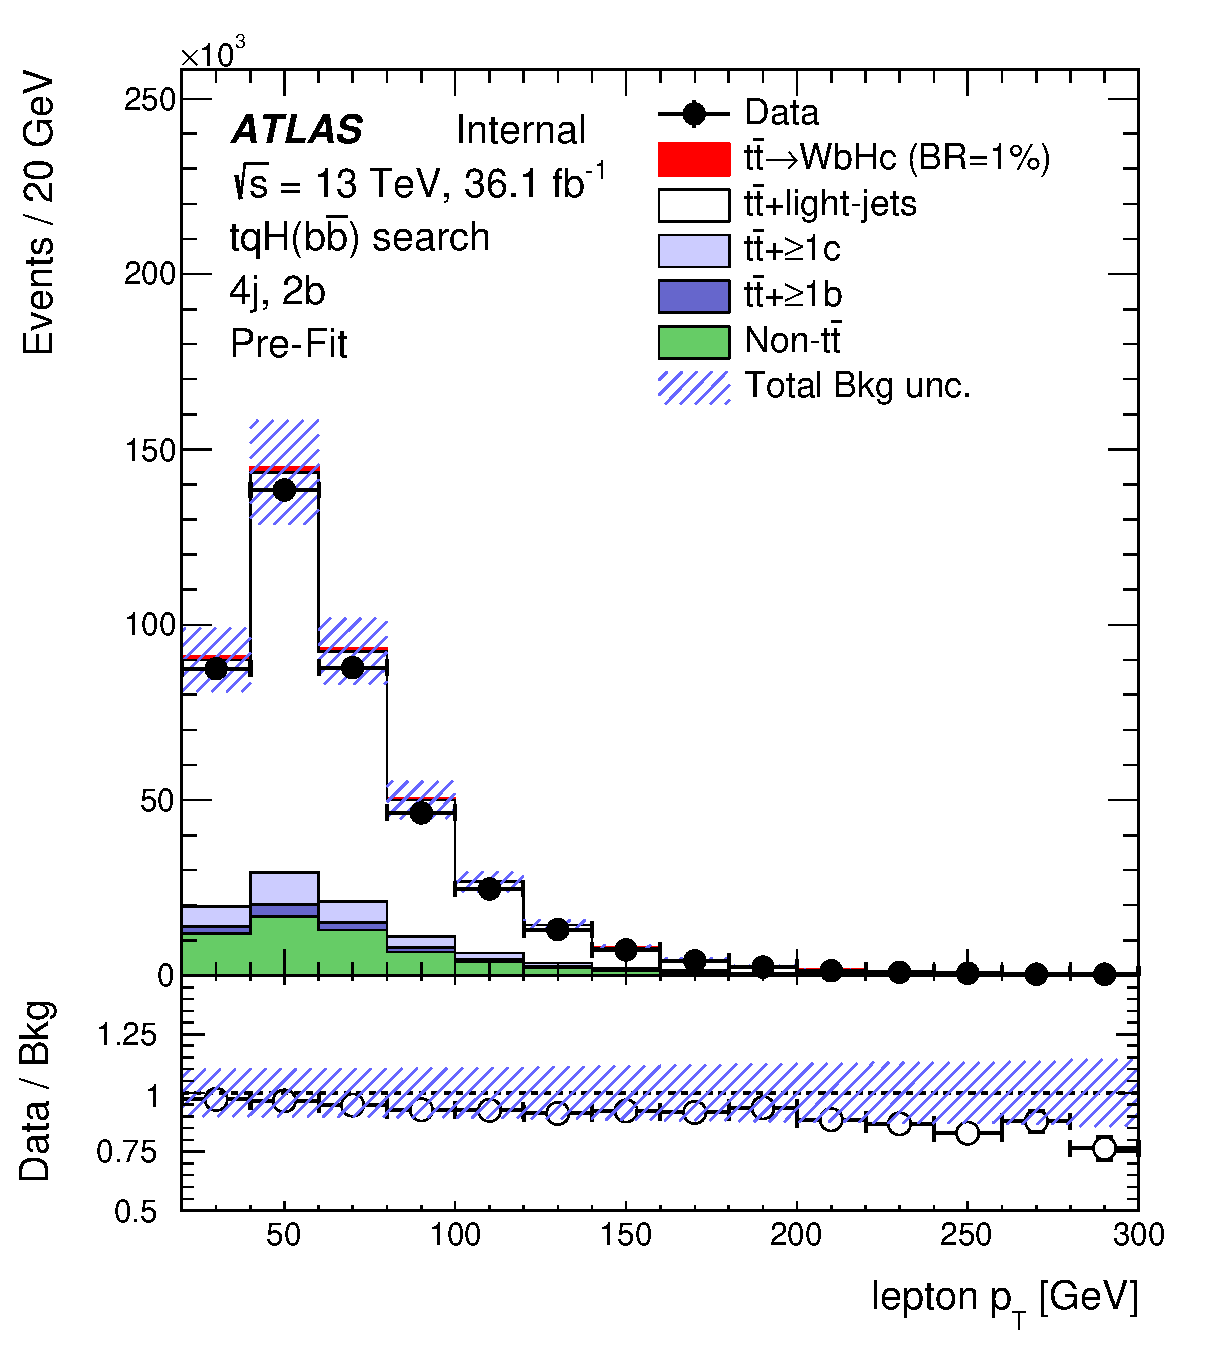
\includegraphics[width=0.40\textwidth]{figures/Hbb/other_variables/c1lep4jex2bex_lep0_pt.eps}}
\subfloat[]{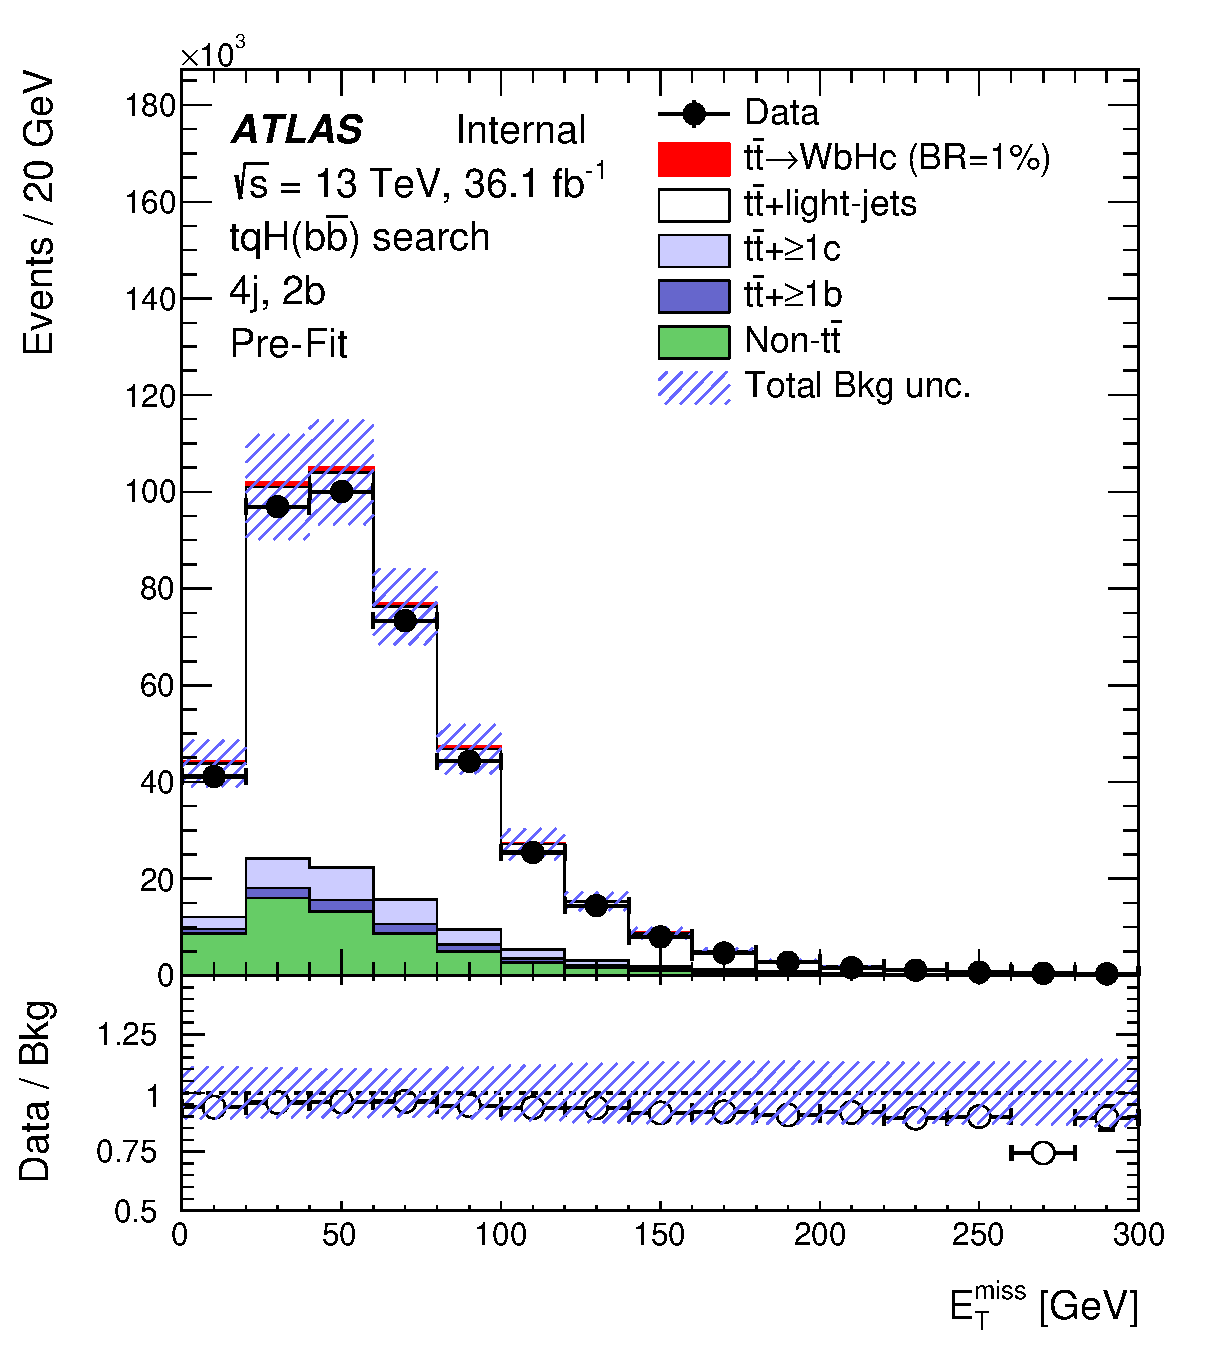
\includegraphics[width=0.40\textwidth]{figures/Hbb/other_variables/c1lep4jex2bex_met.eps}} \\
\subfloat[]{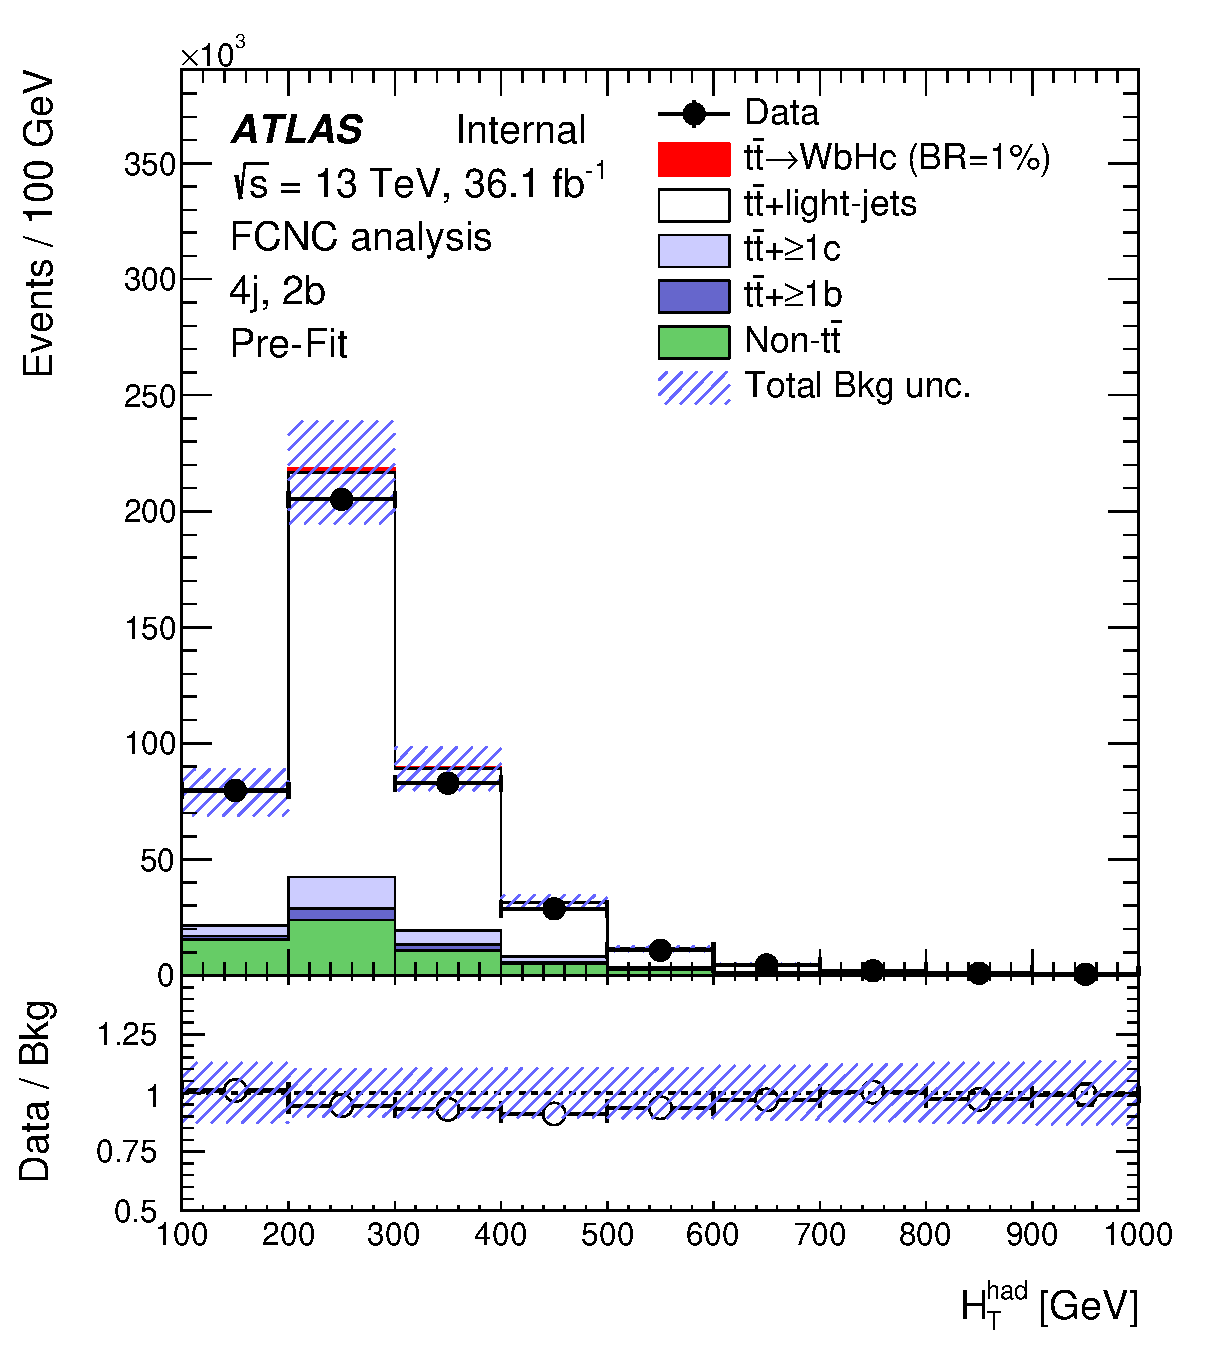
\includegraphics[width=0.40\textwidth]{figures/Hbb/other_variables/c1lep4jex2bex_hthad.eps}} 
\subfloat[]{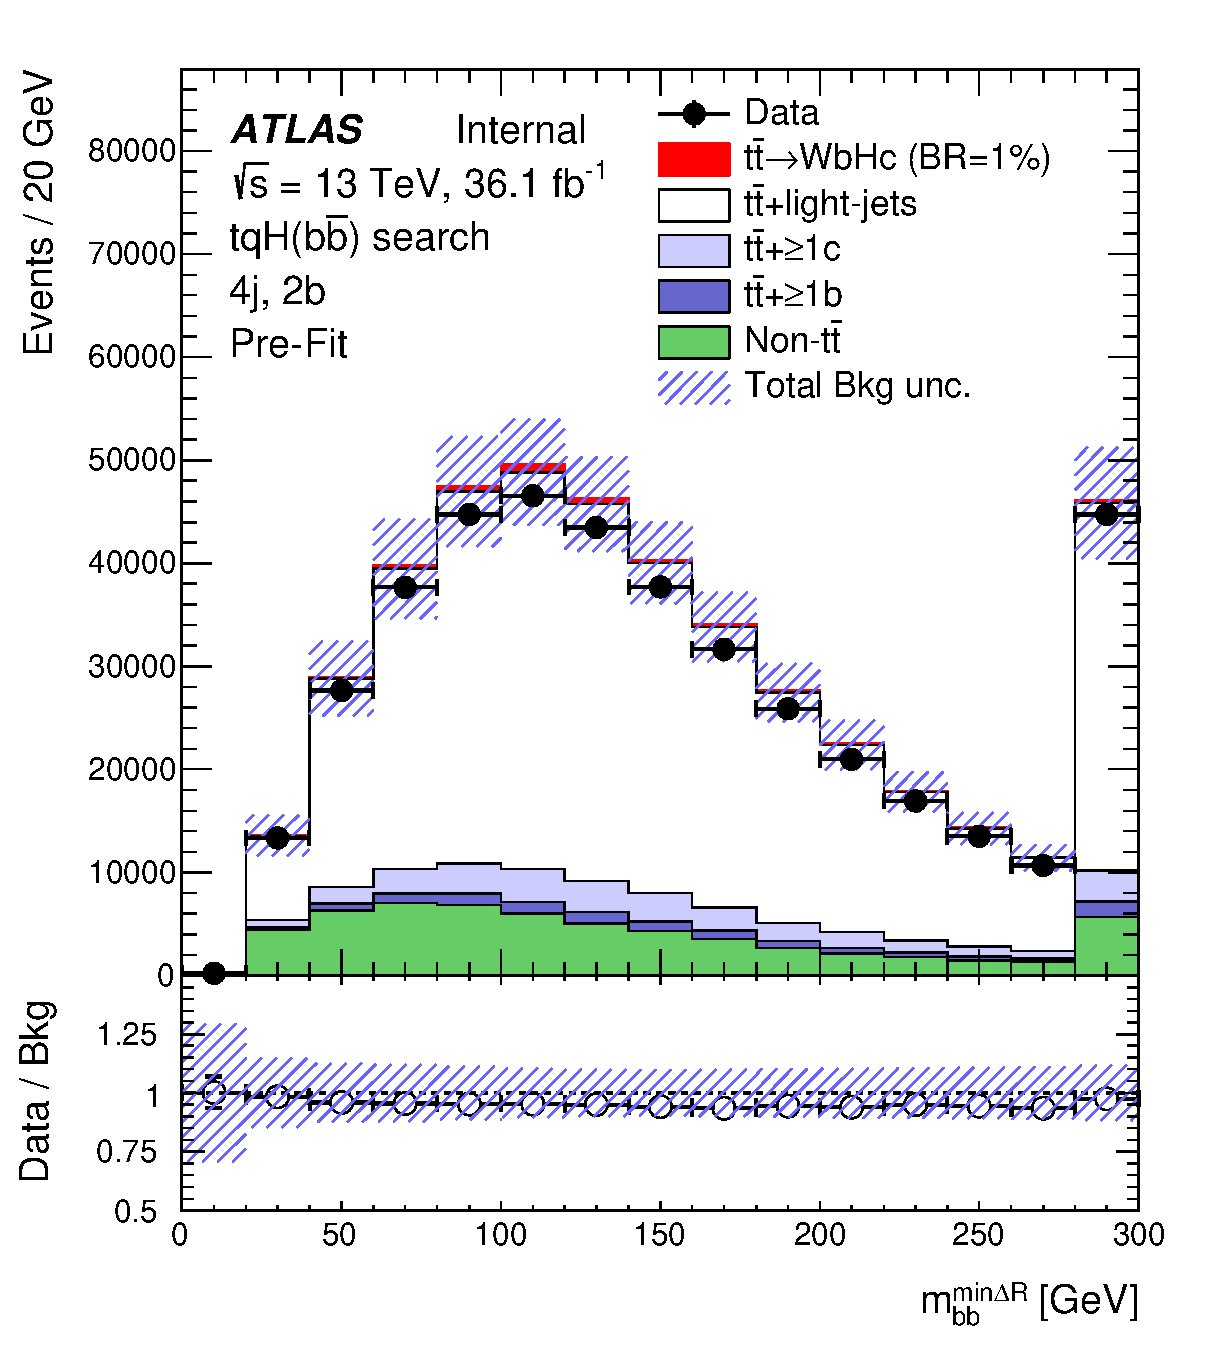
\includegraphics[width=0.40\textwidth]{figures/Hbb/other_variables/c1lep4jex2bex_mbb_mindR.eps}} \\ 
\caption{\small{$\Hbb$ search: Comparison between the data and background prediction for several kinematic 
distributions in the (4j, 2b) region (prior to the application of the cut on the LH discriminant above 0.6) before  the fit to data (``Pre-Fit''). 
The distributions are shown for (a) lepton $\pt$, (b) $\met$, (c) scalar sum of the transverse momenta of 
the jets ($\hthad$), and (d) the invariant mass of the two $b$-tagged jets with lowest 
$\Delta R$ separation ($\mbb$).
The small contributions from $\ttbar V$, $\ttbar H$, single top, $W/Z$+jets, diboson, and multijet backgrounds are combined 
into a single background source referred to as ``Non-$\ttbar$''. 
The expected $\Hc$ signal (solid red) corresponding to $\BR(t\to Hc)=1\%$ is also shown,
added to the background prediction.
The last bin in all figures contains the overflow.
The bottom panel displays the ratio of data to the SM background (``Bkg'') prediction. 
The blue triangles indicate points that are outside the vertical range of the figure. 
The hashed area represents the total uncertainty of the background, excluding the normalisation uncertainty of the $\ttbin$ background, 
which is determined via a likelihood fit to data.}}
\label{fig:Hbb_extravars_4j2b}
\end{center}
\end{figure*}
%%%%%%%%%%%%%%%%%%%%%%%%%%%%%%%%%%%%%%%

%%%%%%%%%%%%%%%%%%%%%%%%%%%%%%%%%%%%%%%%
%\begin{figure*}[htbp]
%\begin{center}
%\subfloat[]{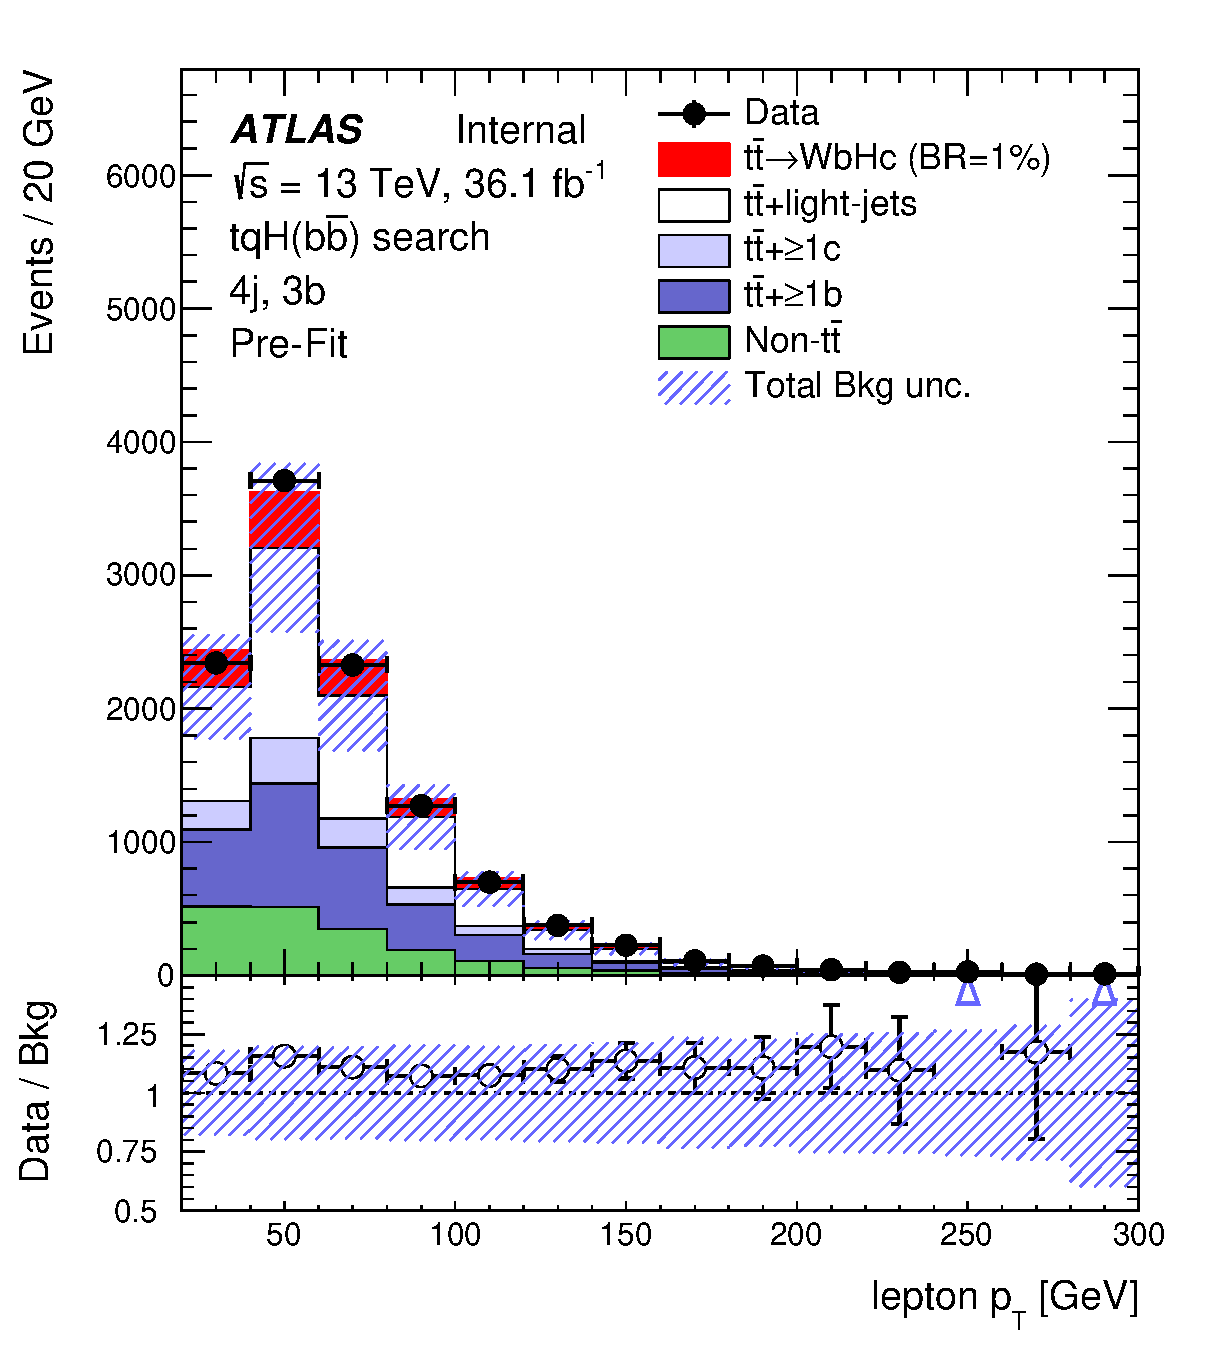
\includegraphics[width=0.40\textwidth]{figures/Hbb/other_variables/c1lep4jex3bex_lep0_pt.eps}}
%\subfloat[]{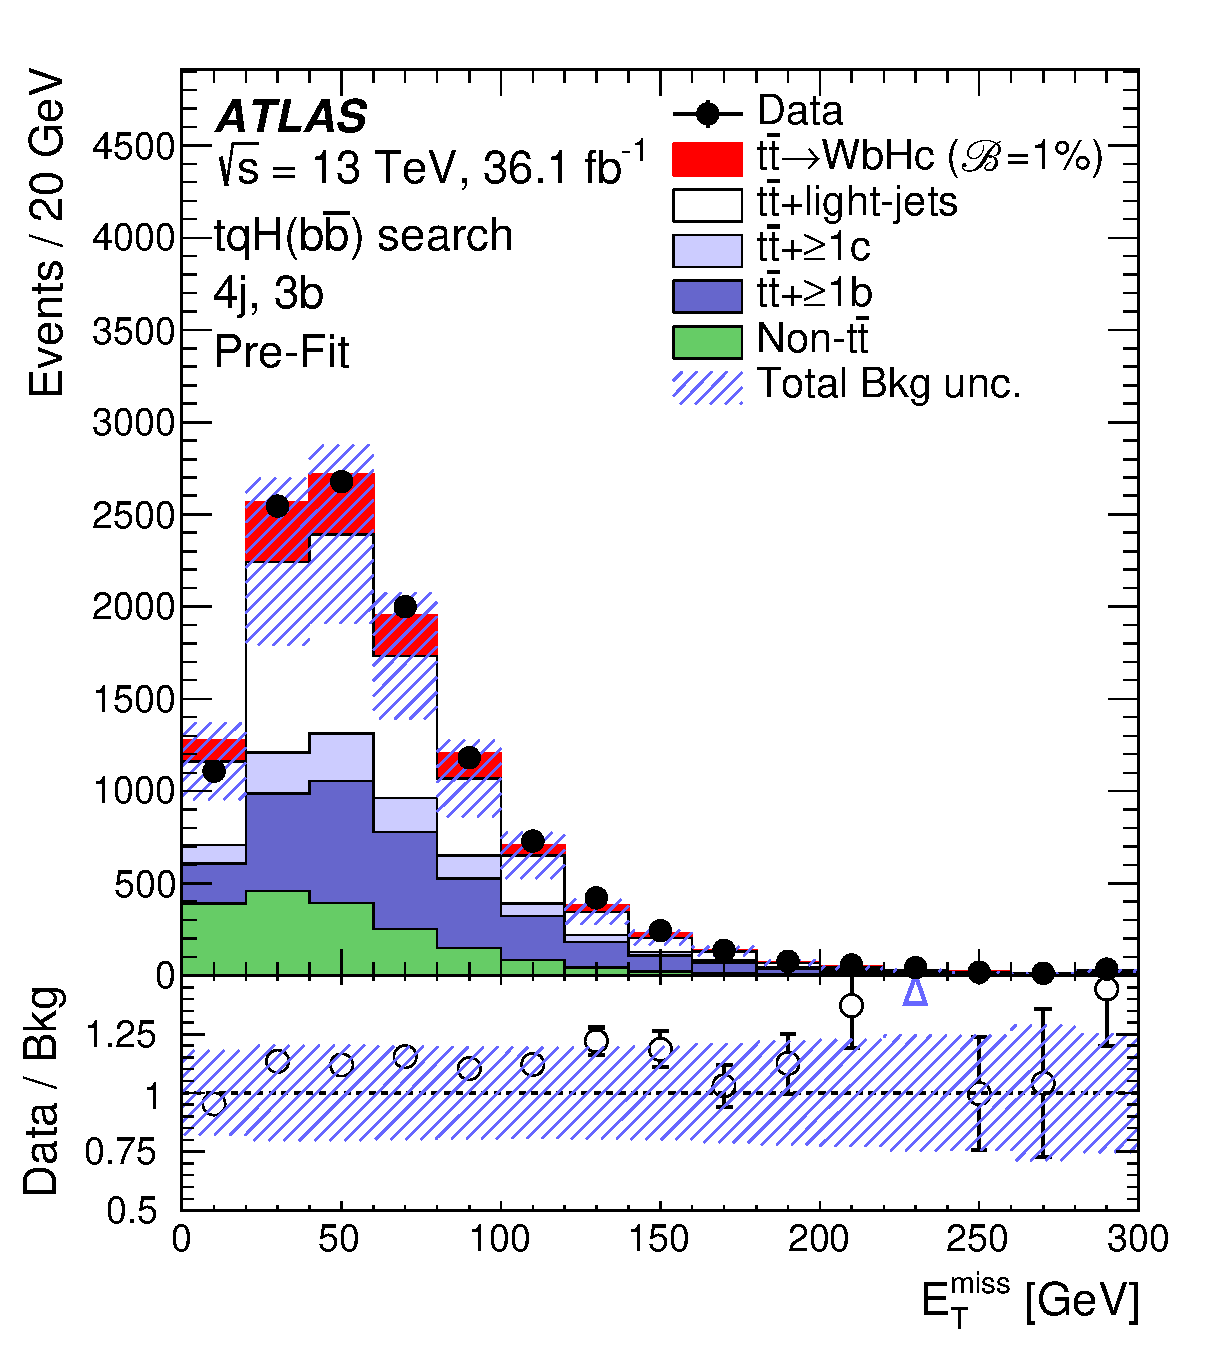
\includegraphics[width=0.40\textwidth]{figures/Hbb/other_variables/c1lep4jex3bex_met.eps}} \\
%\subfloat[]{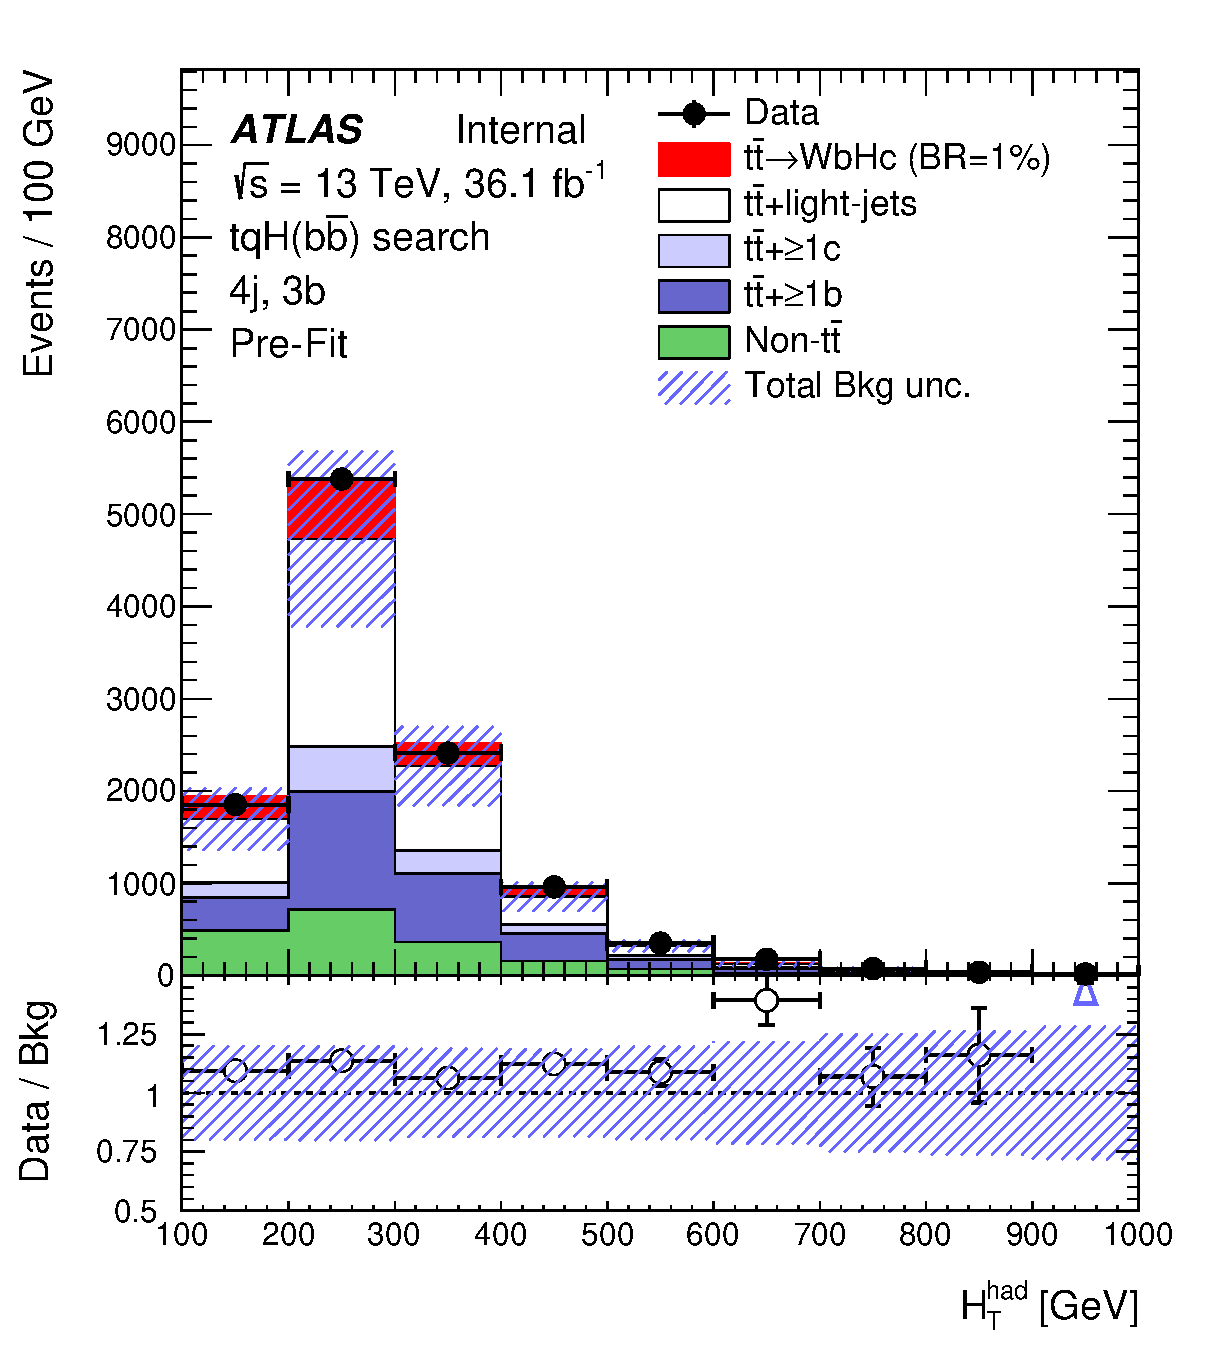
\includegraphics[width=0.40\textwidth]{figures/Hbb/other_variables/c1lep4jex3bex_hthad.eps}} 
%\subfloat[]{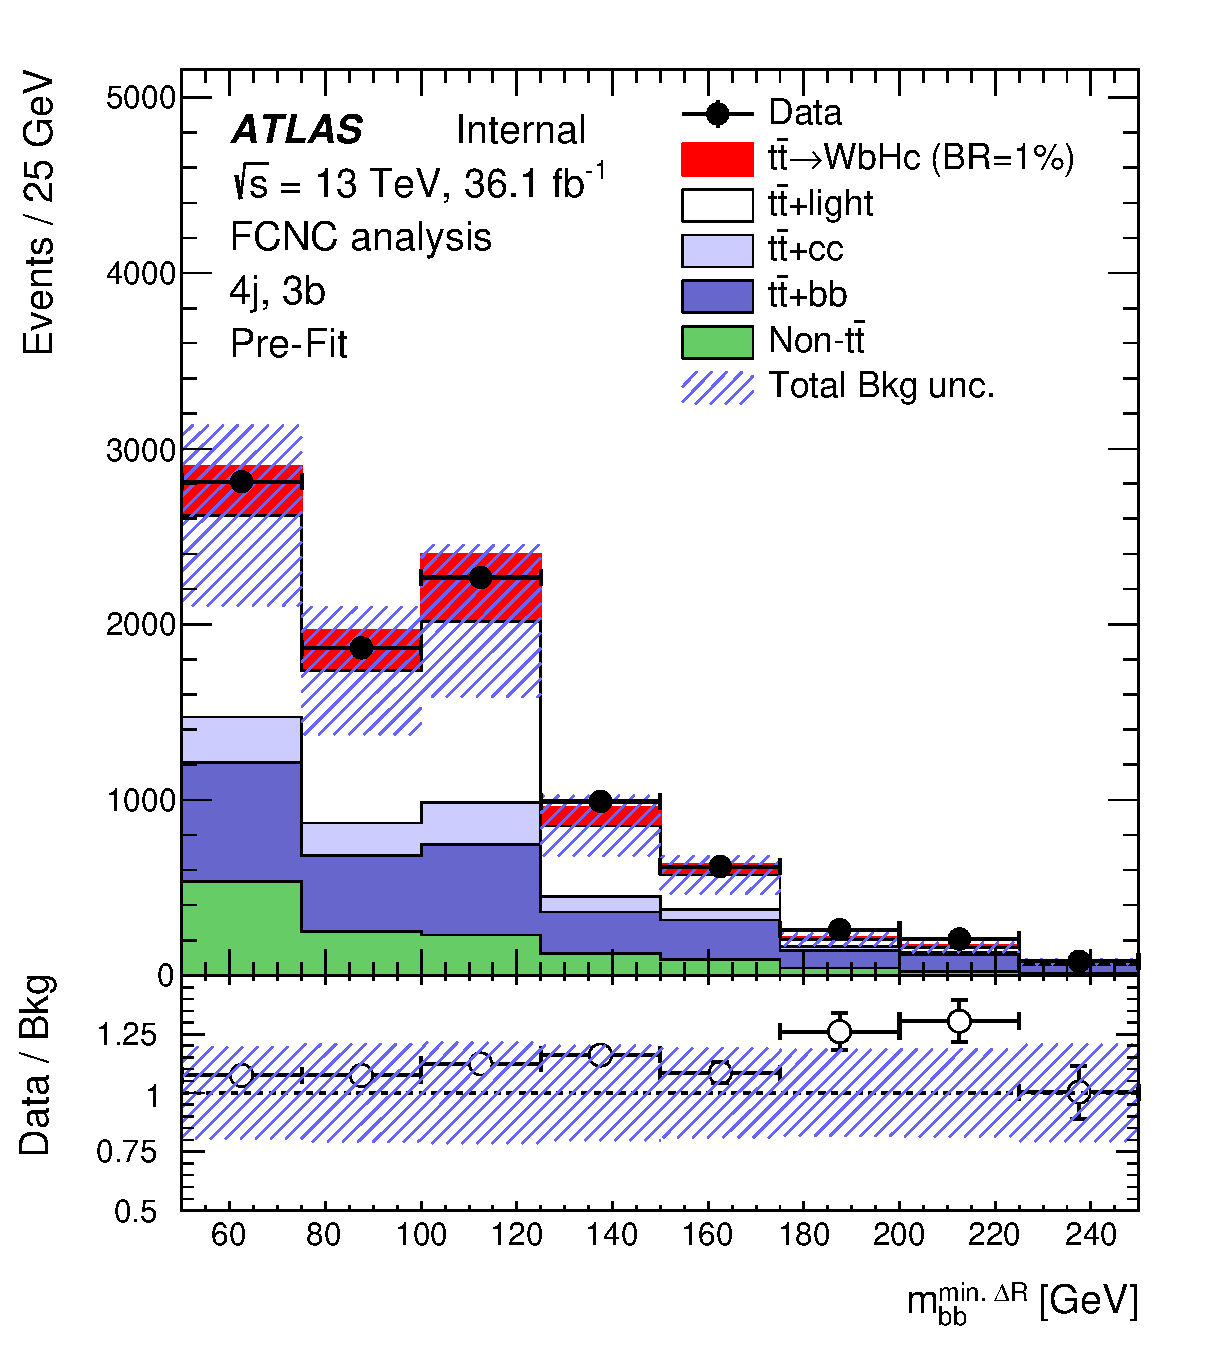
\includegraphics[width=0.40\textwidth]{figures/Hbb/other_variables/c1lep4jex3bex_mbb_mindR.eps}} \\ 
%\caption{\small{$\Hbb$ search: Comparison between the data and background prediction for several kinematic 
%distributions in the (4j, 3b) region before performing the fit to data (``Pre-Fit''). 
%The distributions are shown for (a) lepton $\pt$, (b) $\met$, (c) scalar sum of the transverse momenta of 
%the jets ($\hthad$), and (d) the invariant mass distribution of the two $b$-tagged jets with lowest 
%$\Delta R$ separation ($\mbb$).
%The small contributions from $\ttbar V$, $\ttbar H$, single top, $W/Z$+jets, diboson, and multijet backgrounds are combined 
%into a single background source referred to as ``Non-$\ttbar$''. 
%The expected $\Hc$ signal (solid red) corresponding to $\BR(t\to Hc)=1\%$ is also shown,
%added on top of the background prediction.
%The last bin in all figures contains the overflow.
%The bottom panel displays the ratio of data to the SM background (``Bkg'') prediction. 
%The blue triangles indicate points that are outside the vertical range of the figure. 
%The hashed area represents the total uncertainty on the background, excluding the normalisation uncertainty of the $\ttbin$ background, 
%which is determined via a likelihood fit to data.}}
%\label{fig:Hbb_extravars_4j3b}
%\end{center}
%\end{figure*}
%%%%%%%%%%%%%%%%%%%%%%%%%%%%%%%%%%%%%%%%

%%%%%%%%%%%%%%%%%%%%%%%%%%%%%%%%%%%%%%%
\begin{figure*}[htbp]
\begin{center}
\subfloat[]{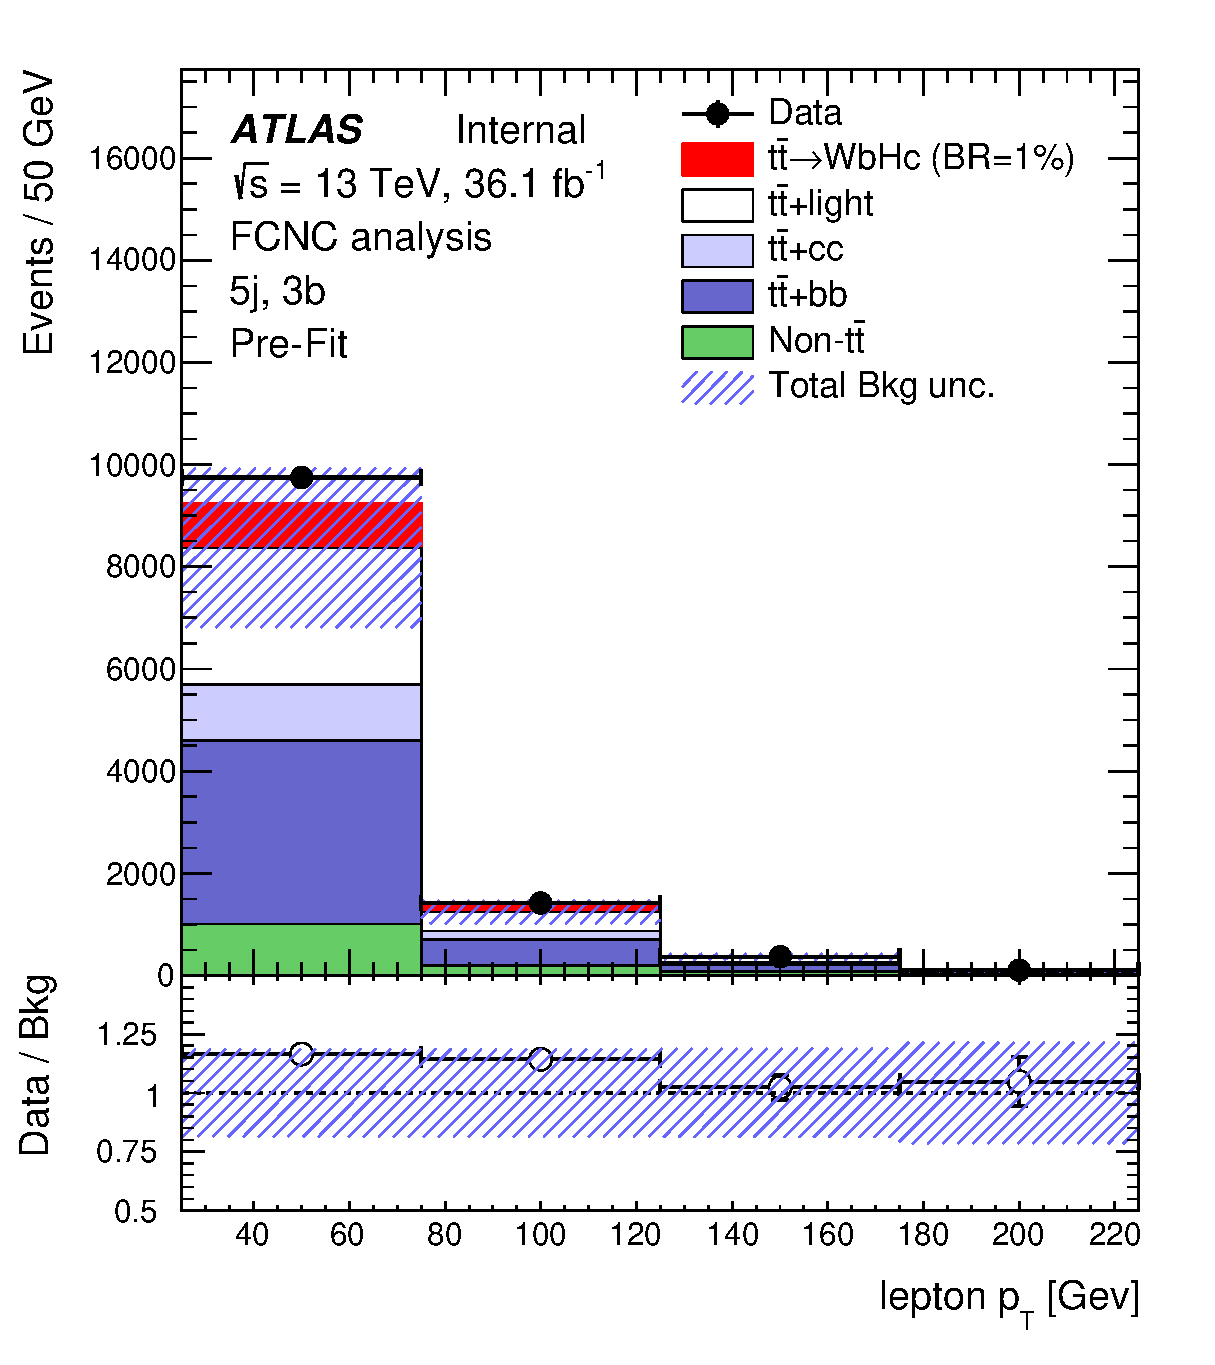
\includegraphics[width=0.40\textwidth]{figures/Hbb/other_variables/c1lep5jex3bex_lep0_pt.eps}}
\subfloat[]{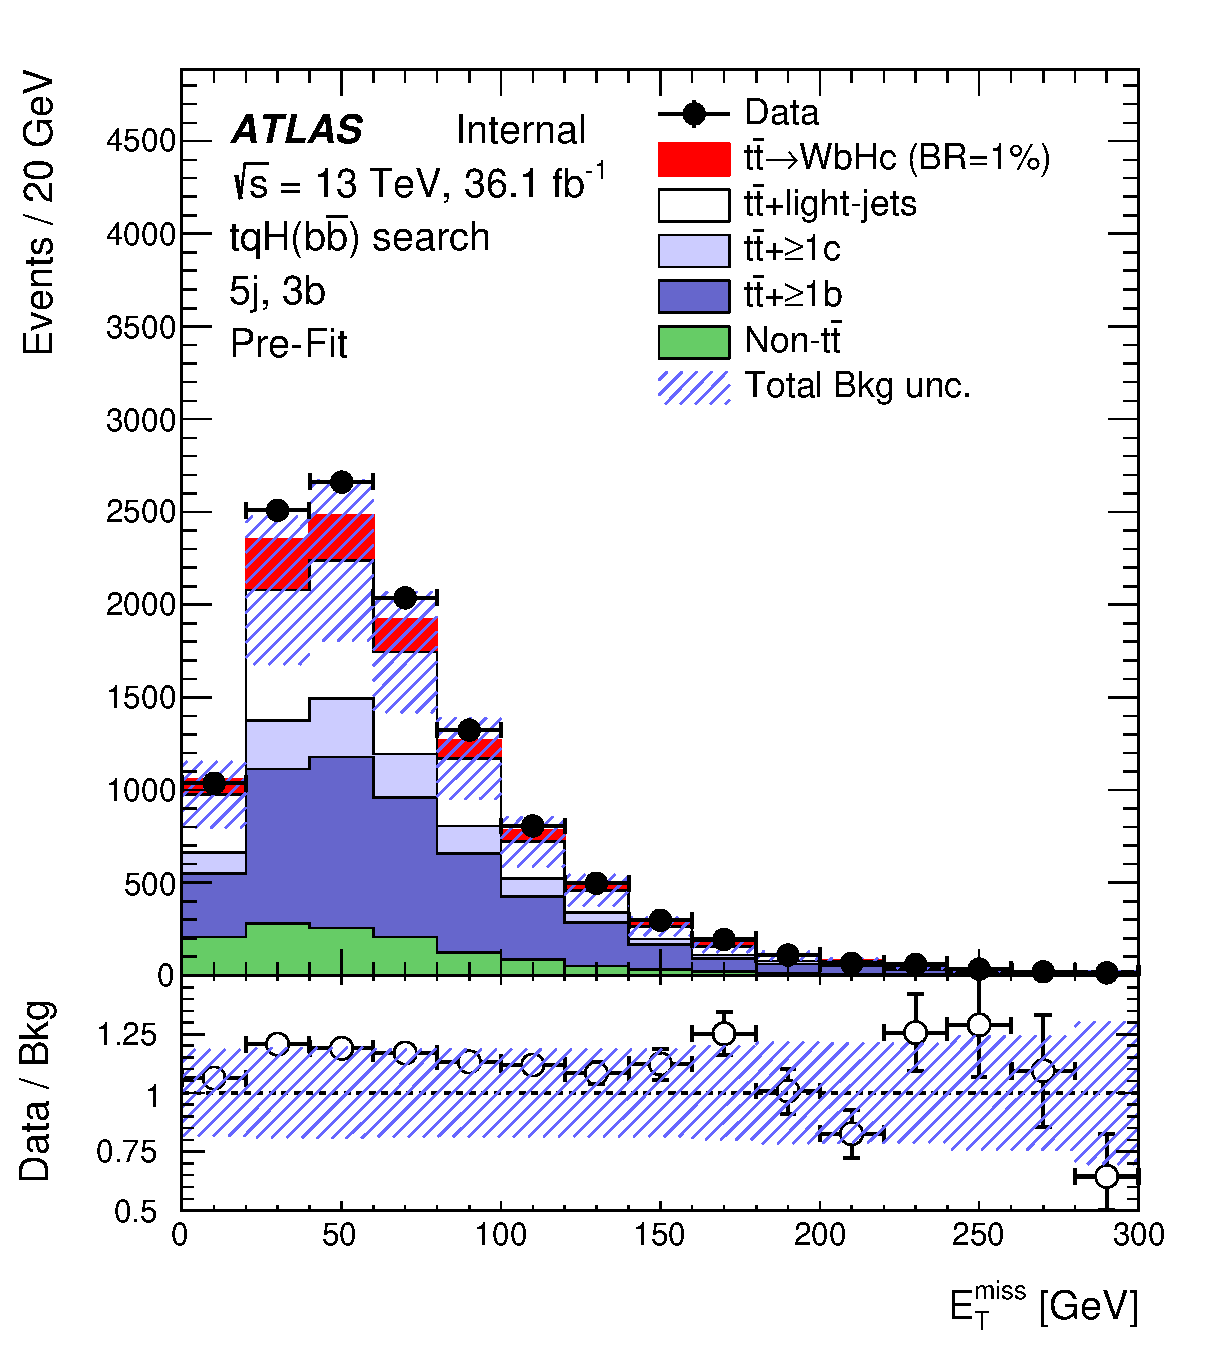
\includegraphics[width=0.40\textwidth]{figures/Hbb/other_variables/c1lep5jex3bex_met.eps}} \\
\subfloat[]{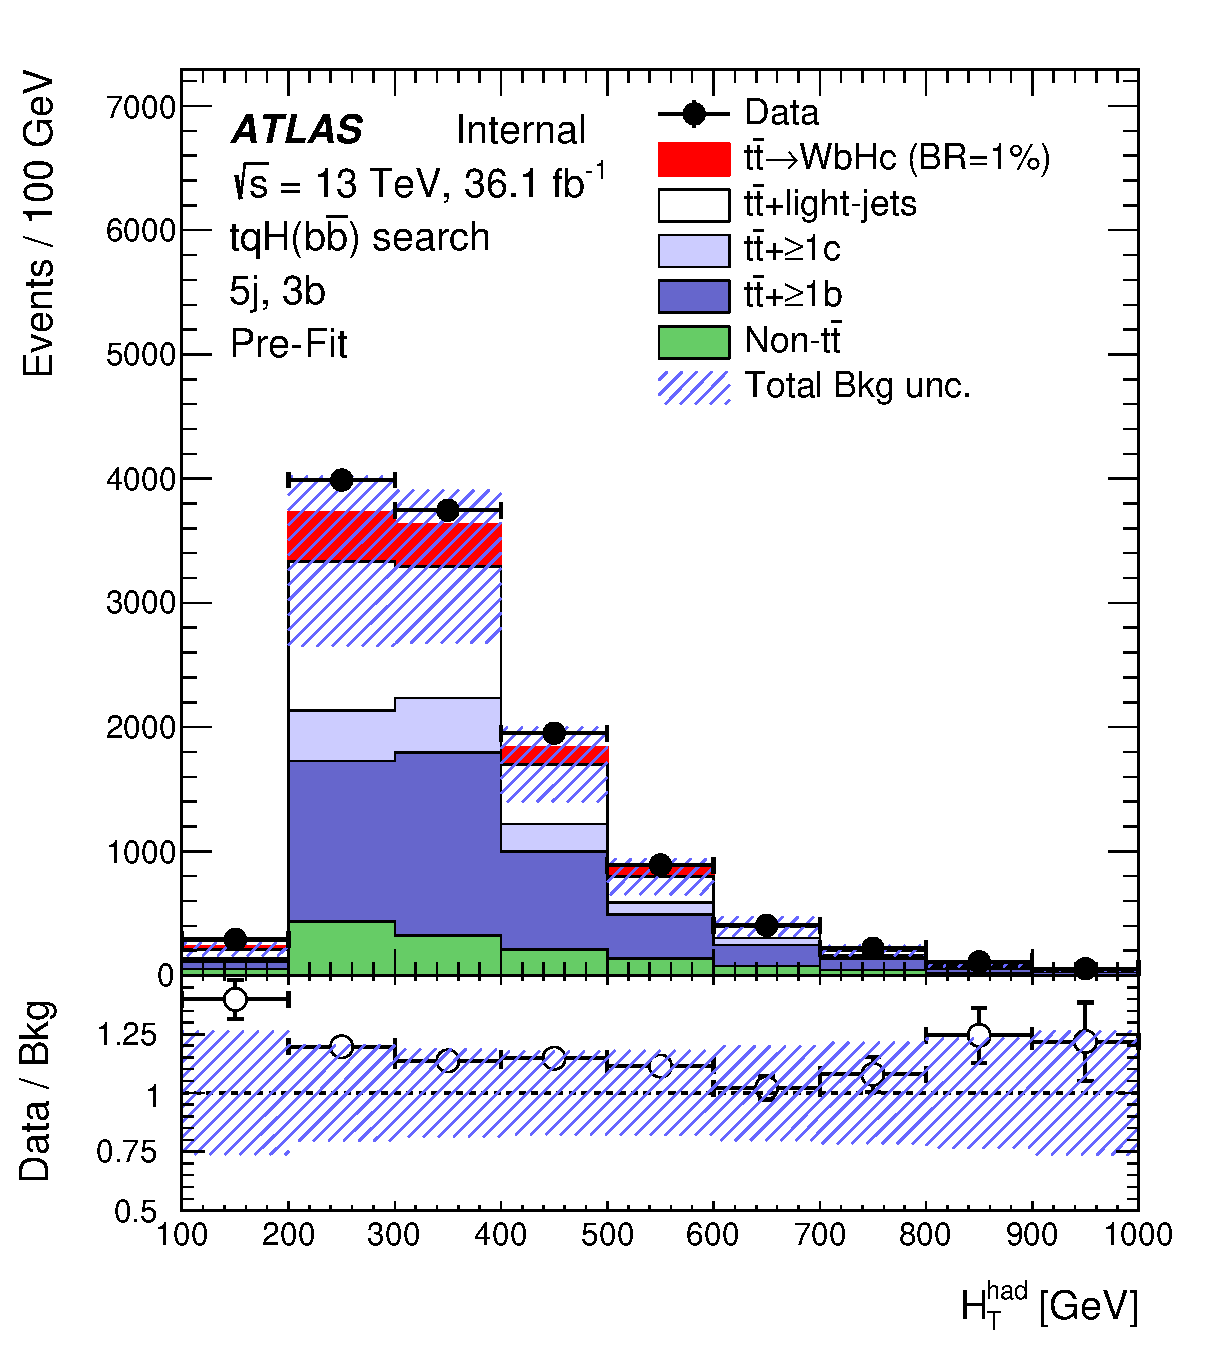
\includegraphics[width=0.40\textwidth]{figures/Hbb/other_variables/c1lep5jex3bex_hthad.eps}} 
\subfloat[]{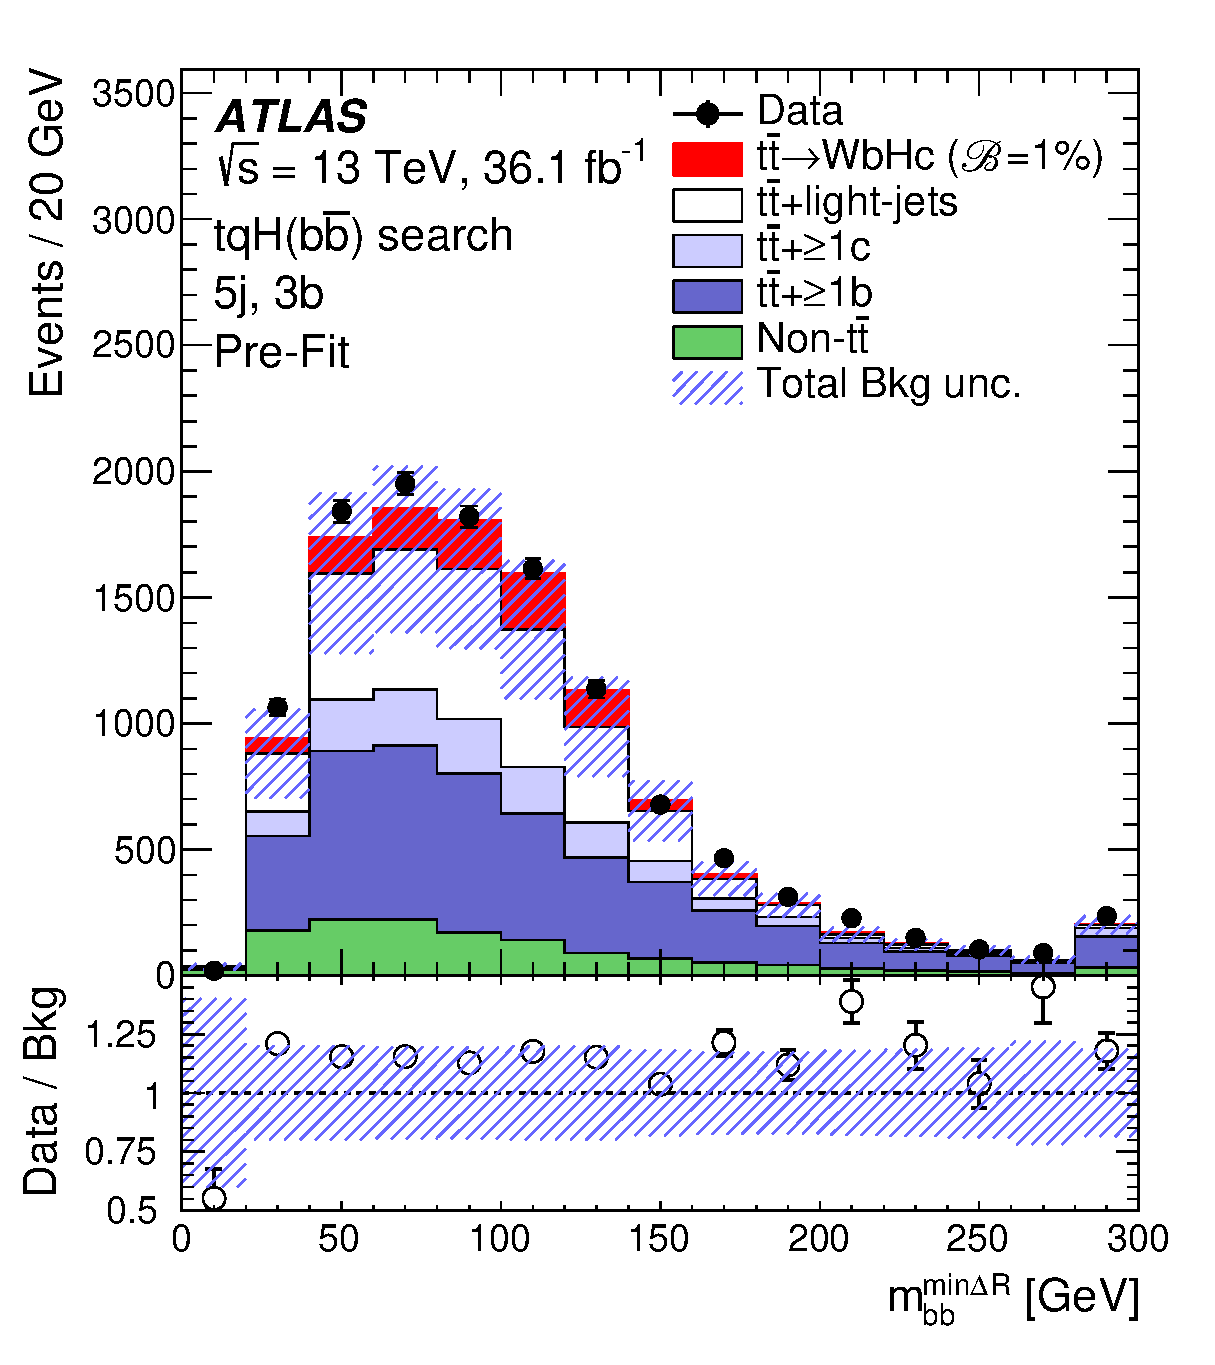
\includegraphics[width=0.40\textwidth]{figures/Hbb/other_variables/c1lep5jex3bex_mbb_mindR.eps}} \\ 
\caption{\small{$\Hbb$ search: Comparison between the data and background prediction for several kinematic 
distributions in the (5j, 3b) region before the fit to data (``Pre-Fit''). 
The distributions are shown for (a) lepton $\pt$, (b) $\met$, (c) scalar sum of the transverse momenta of 
the jets ($\hthad$), and (d) the invariant mass of the two $b$-tagged jets with lowest 
$\Delta R$ separation ($\mbb$).
The small contributions from $\ttbar V$, $\ttbar H$, single top, $W/Z$+jets, diboson, and multijet backgrounds are combined 
into a single background source referred to as ``Non-$\ttbar$''. 
The expected $\Hc$ signal (solid red) corresponding to $\BR(t\to Hc)=1\%$ is also shown,
added to the background prediction.
The last bin in all figures contains the overflow.
The bottom panel displays the ratio of data to the SM background (``Bkg'') prediction. 
The blue triangles indicate points that are outside the vertical range of the figure. 
The hashed area represents the total uncertainty of the background, excluding the normalisation uncertainty of the $\ttbin$ background, 
which is determined via a likelihood fit to data.}}
\label{fig:Hbb_extravars_5j3b}
\end{center}
\end{figure*}
%%%%%%%%%%%%%%%%%%%%%%%%%%%%%%%%%%%%%%%

%%%%%%%%%%%%%%%%%%%%%%%%%%%%%%%%%%%%%%%
\begin{figure*}[t]
\begin{center}
\subfloat[]{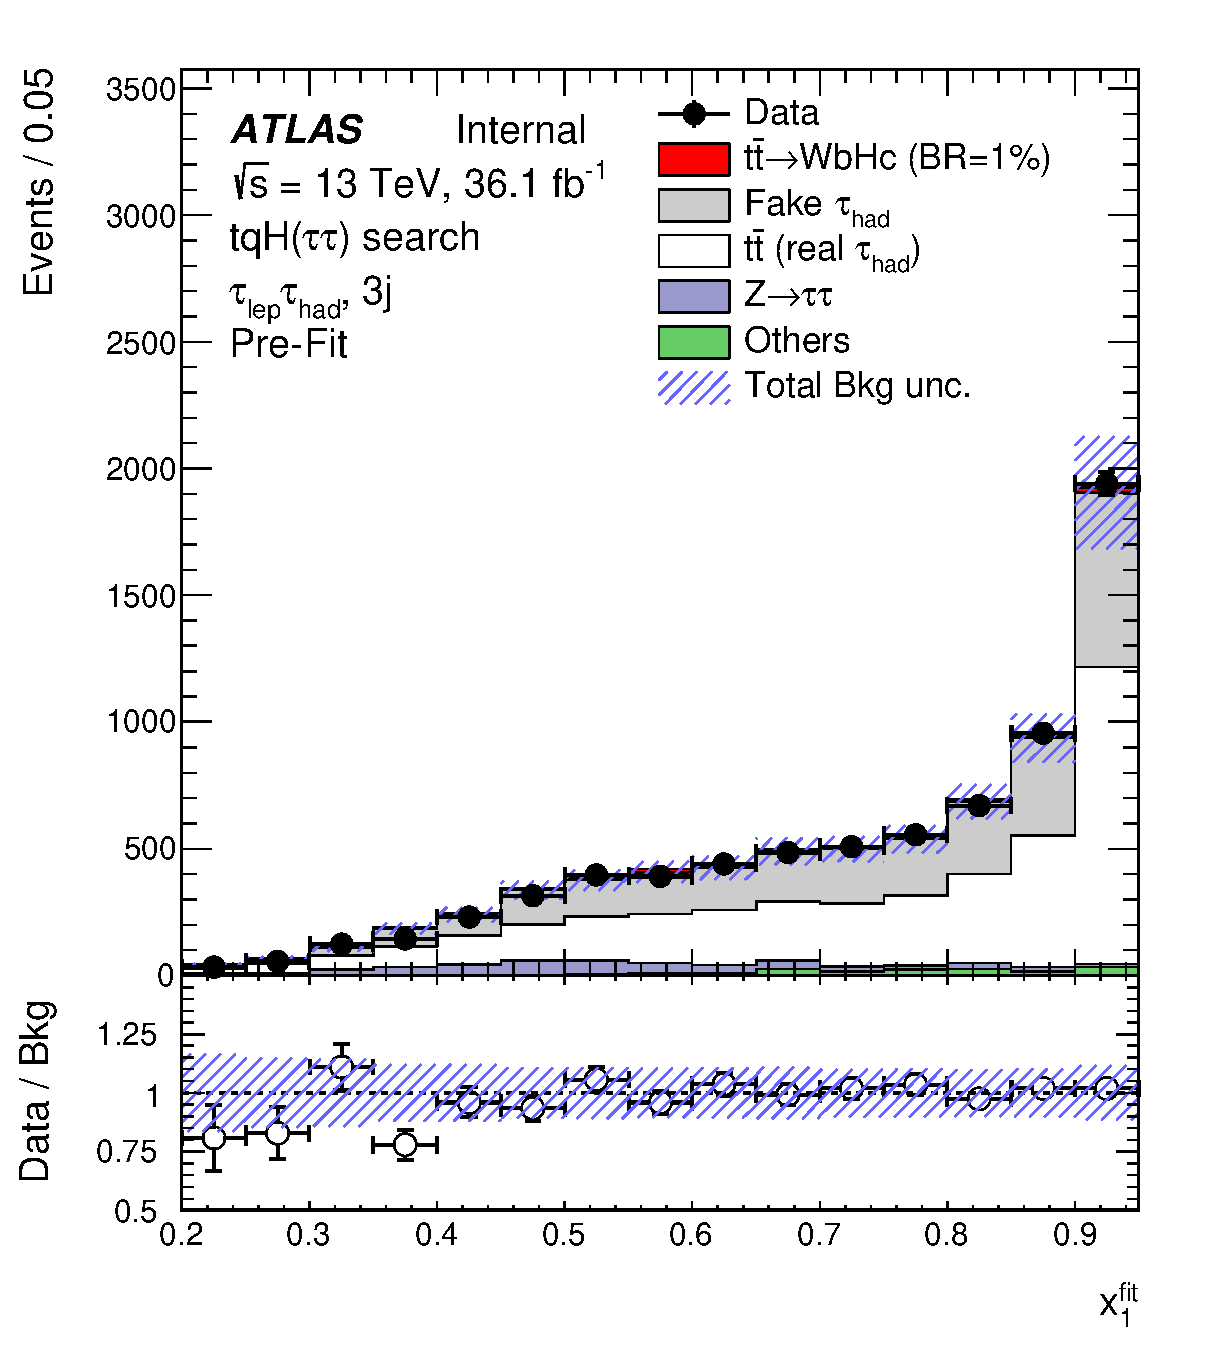
\includegraphics[width=0.40\textwidth]{figures/Htautau/control_plots/x1_fit_lephad_3j_FR.eps}}
\subfloat[]{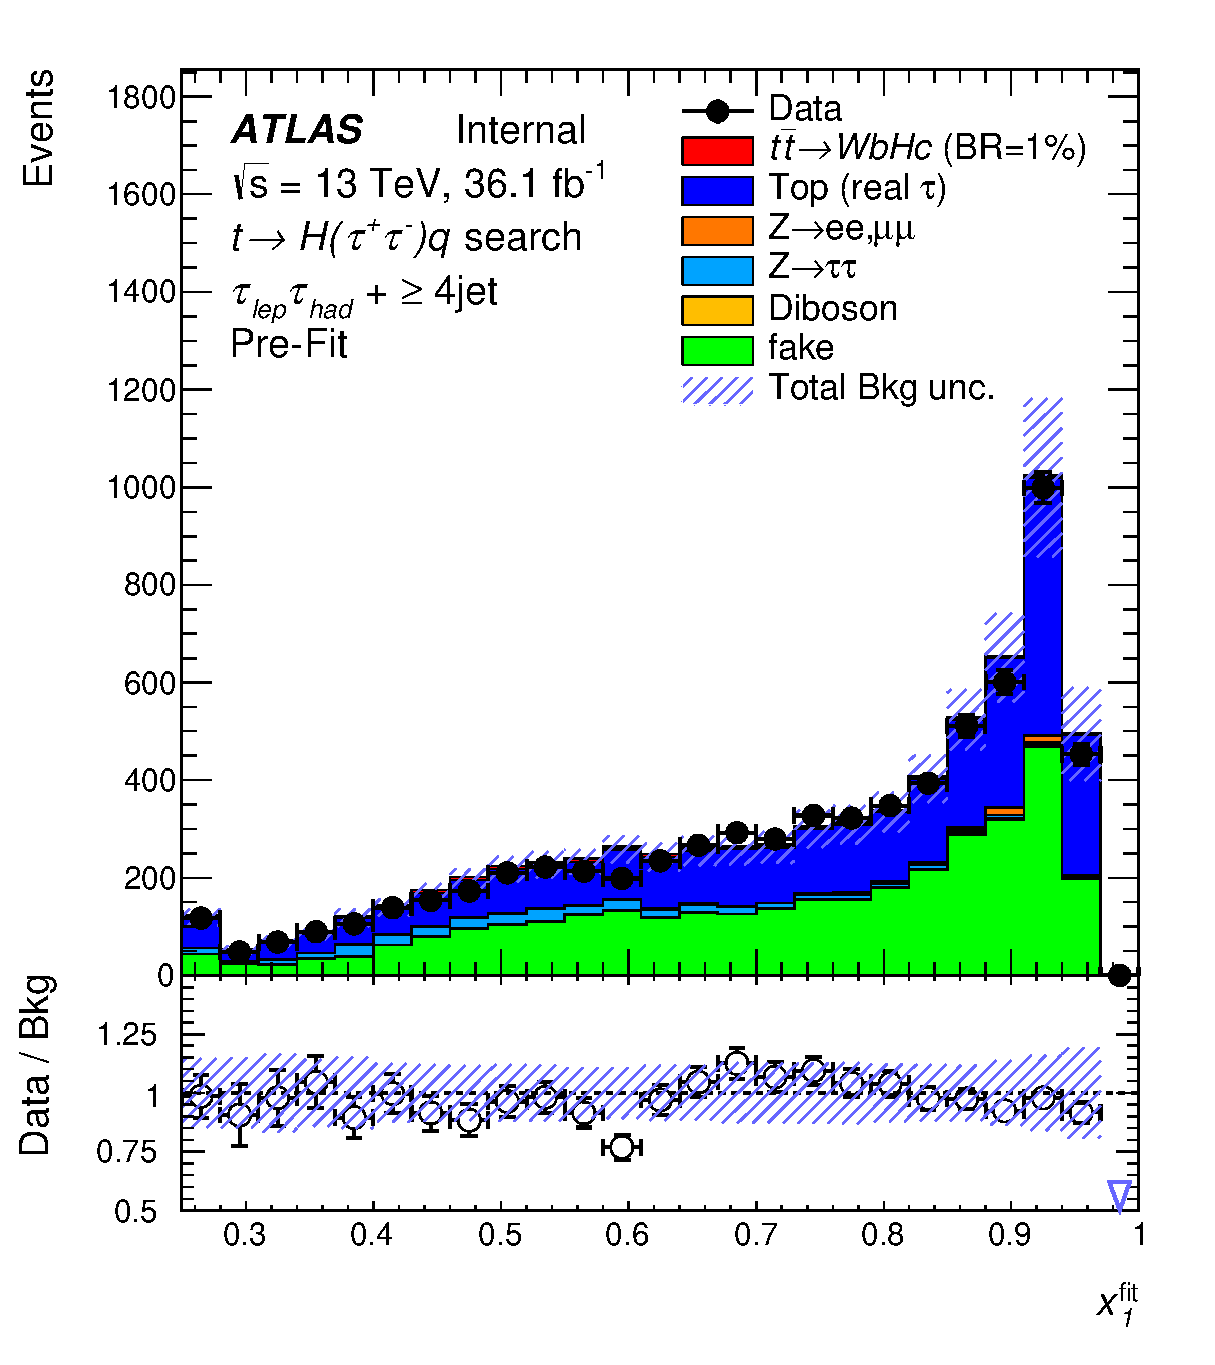
\includegraphics[width=0.40\textwidth]{figures/Htautau/control_plots/x1_fit_lephad_4j_FR.eps}} \\
\subfloat[]{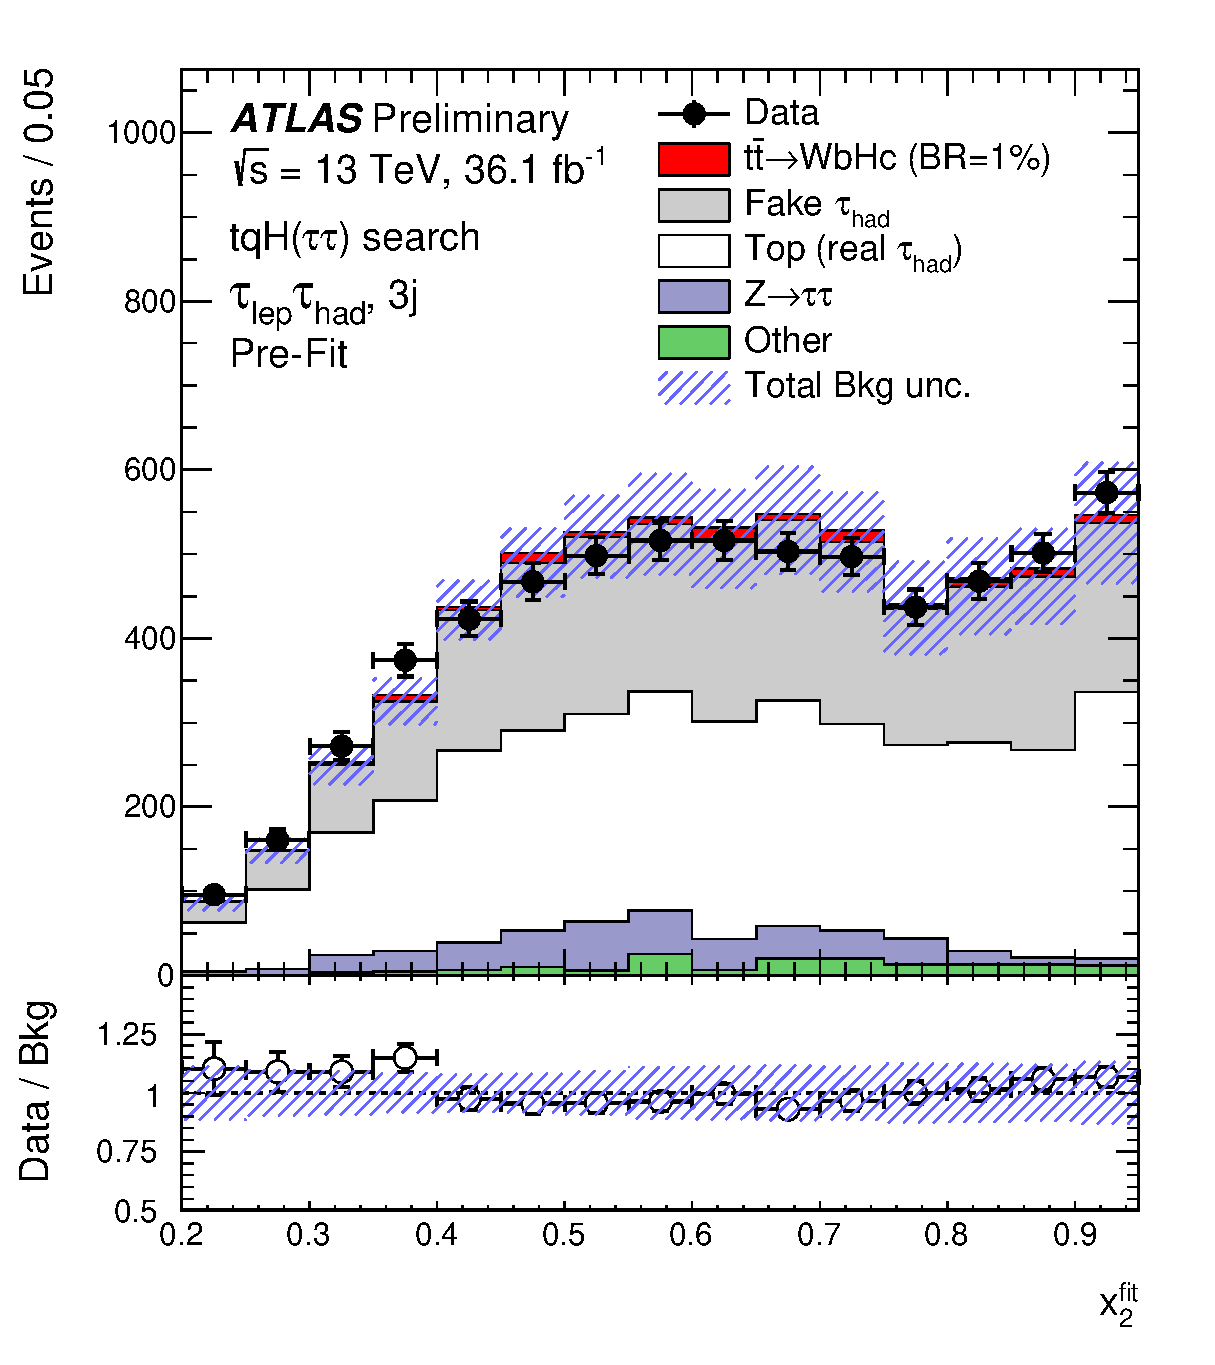
\includegraphics[width=0.40\textwidth]{figures/Htautau/control_plots/x2_fit_lephad_3j_FR.eps}}
\subfloat[]{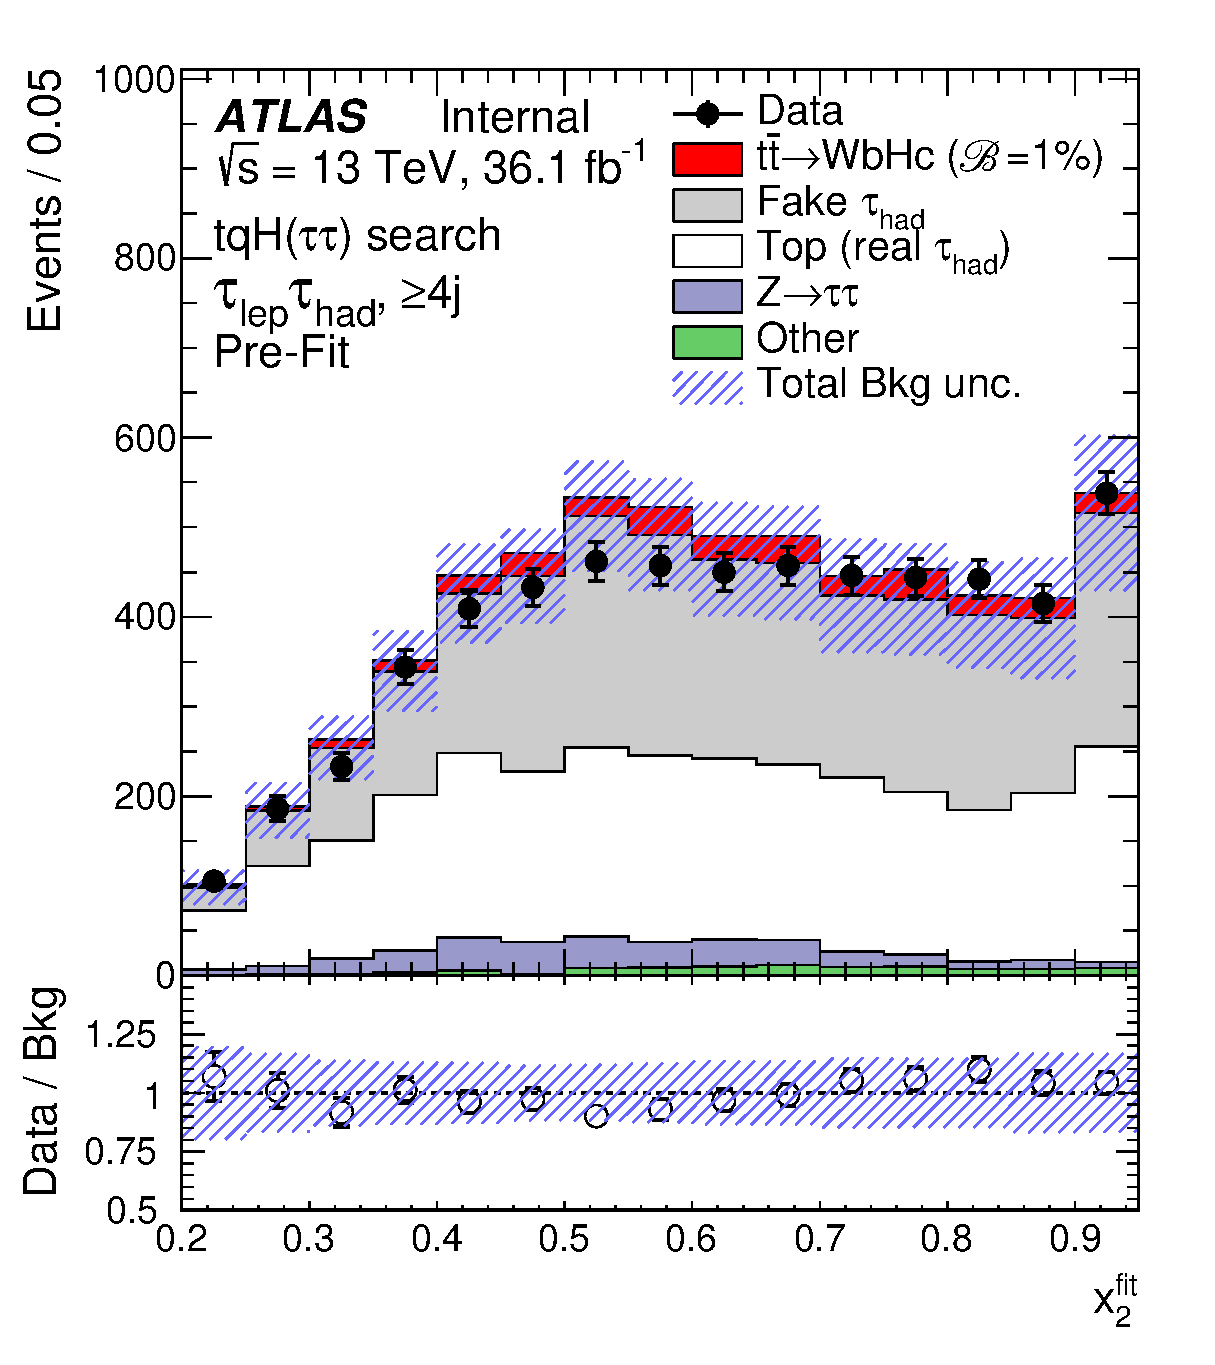
\includegraphics[width=0.40\textwidth]{figures/Htautau/control_plots/x2_fit_lephad_4j_FR.eps}} \\
\caption{$\Htautau$ search: Comparison between the data and background prediction for the distribution of some of the most
discriminating BDT input variables in the $\lephad$ channel before the fit to data (``Pre-Fit''). The distributions are shown for
$x_{1}^{\text{fit}}$ in (a) the ($\lephad$, 3j) region and (b) the ($\lephad$, $\geq$4j) region, and for
$x_{2}^{\text{fit}}$ in (c) the ($\lephad$, 3j)  region and (d) the ($\lephad$, $\geq$4j) region.
The contributions with real $\had$ candidates from $\ttbar$,  $\ttbar V$, $\ttbar H$, and single top backgrounds are combined into
a single background source referred to as ``Top (real $\had$)", whereas the small contributions from 
$Z\to \ell^+\ell^-$ ($\ell = e, \mu$) and diboson backgrounds are combined into ``Other''. 
The expected $\Hc$ signal (solid red) corresponding to $\BR(t\to Hc)=1\%$ is also shown,
added to the background prediction.
%The first and the last bins in all figures contain the underflow and overflow respectively.
The bottom panel displays the ratio of data to the SM background (``Bkg'') prediction.
The hashed area represents the total uncertainty of the background, excluding the normalisation uncertainty of the fake $\had$ background, 
which is determined via a likelihood fit to data.}
\label{fig:BDT_inputs_lephad_2}
\end{center}
\end{figure*}
%%%%%%%%%%%%%%%%%%%%%%%%%%%%%%%%%%%%%%%


%%%%%%%%%%%%%%%%%%%%%%%%%%%%%%%%%%%%%%%
\begin{figure*}[t]
\begin{center}
\subfloat[]{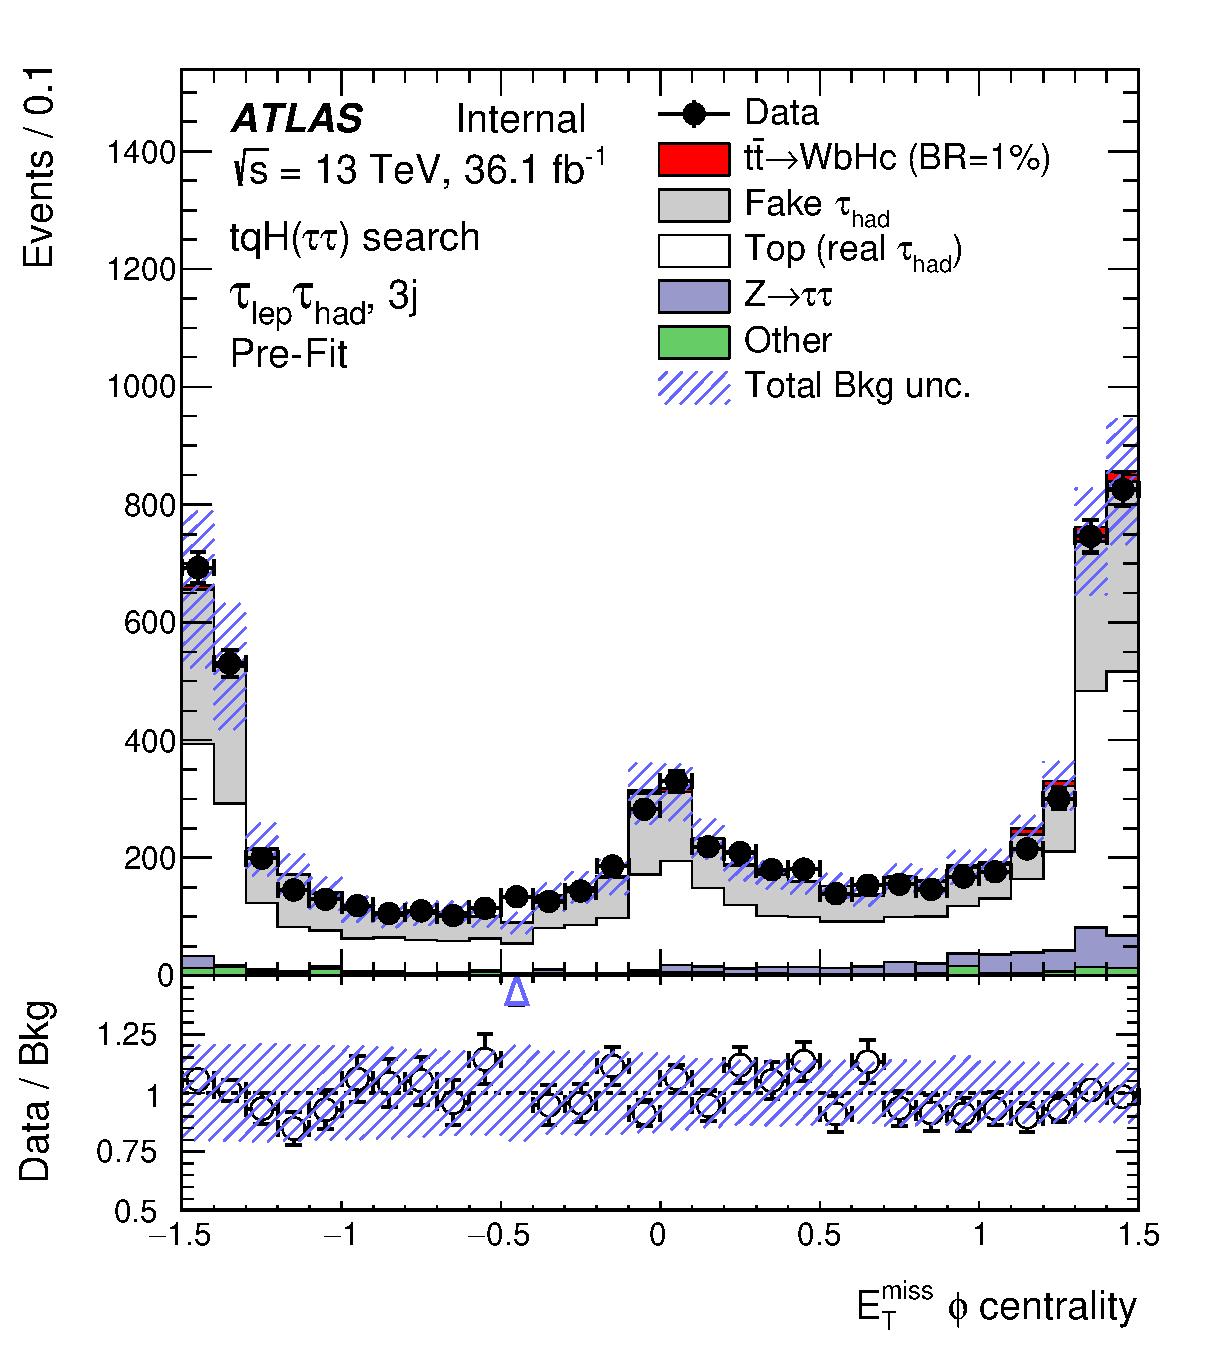
\includegraphics[width=0.40\textwidth]{figures/Htautau/control_plots/met_centrality_lephad_3j_FR.eps}}
\subfloat[]{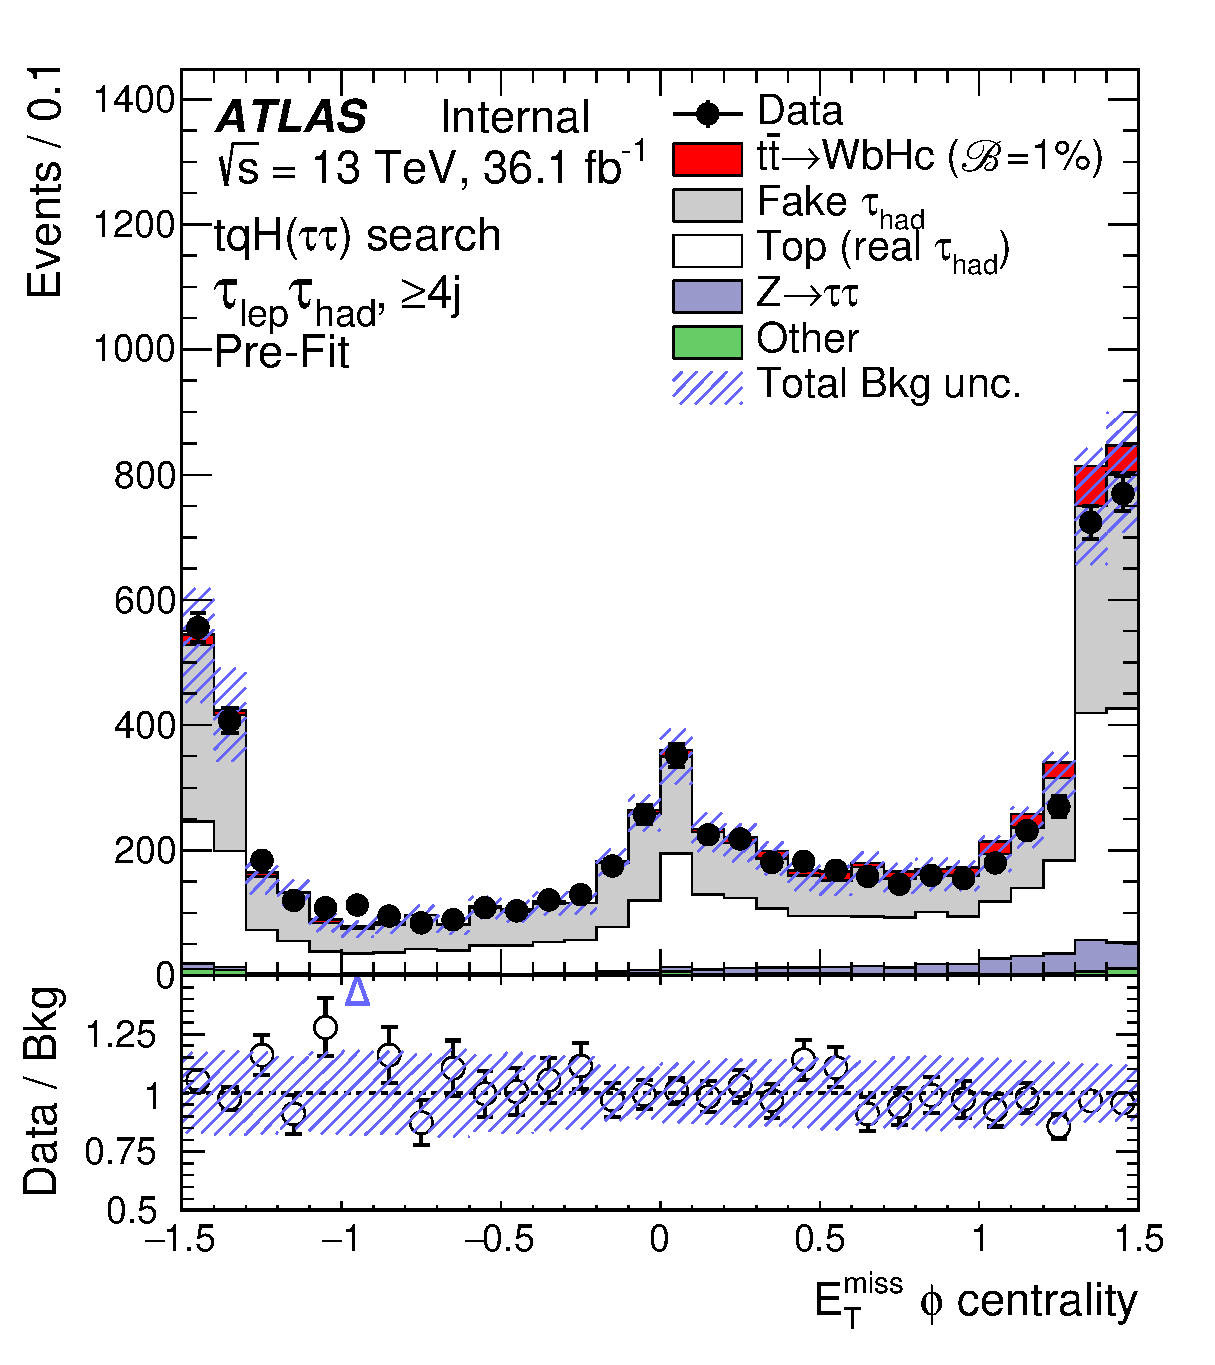
\includegraphics[width=0.40\textwidth]{figures/Htautau/control_plots/met_centrality_lephad_4j_FR.eps}} \\
\subfloat[]{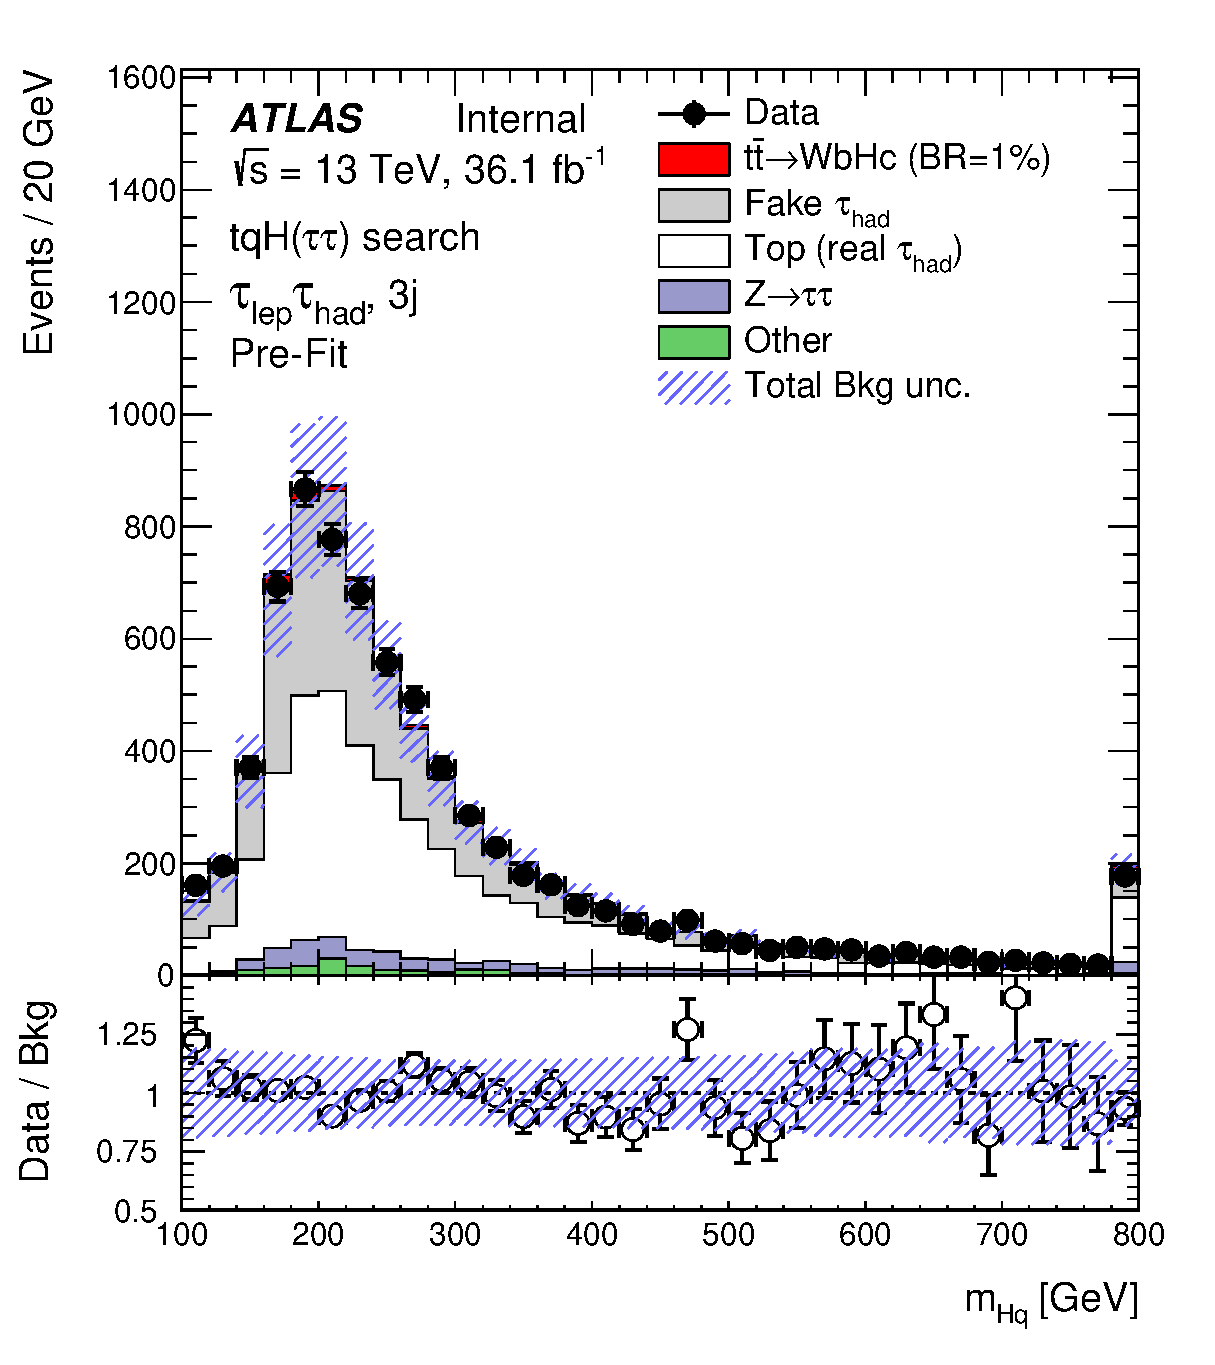
\includegraphics[width=0.40\textwidth]{figures/Htautau/control_plots/mtop_thc_lephad_3j_FR.eps}}
\subfloat[]{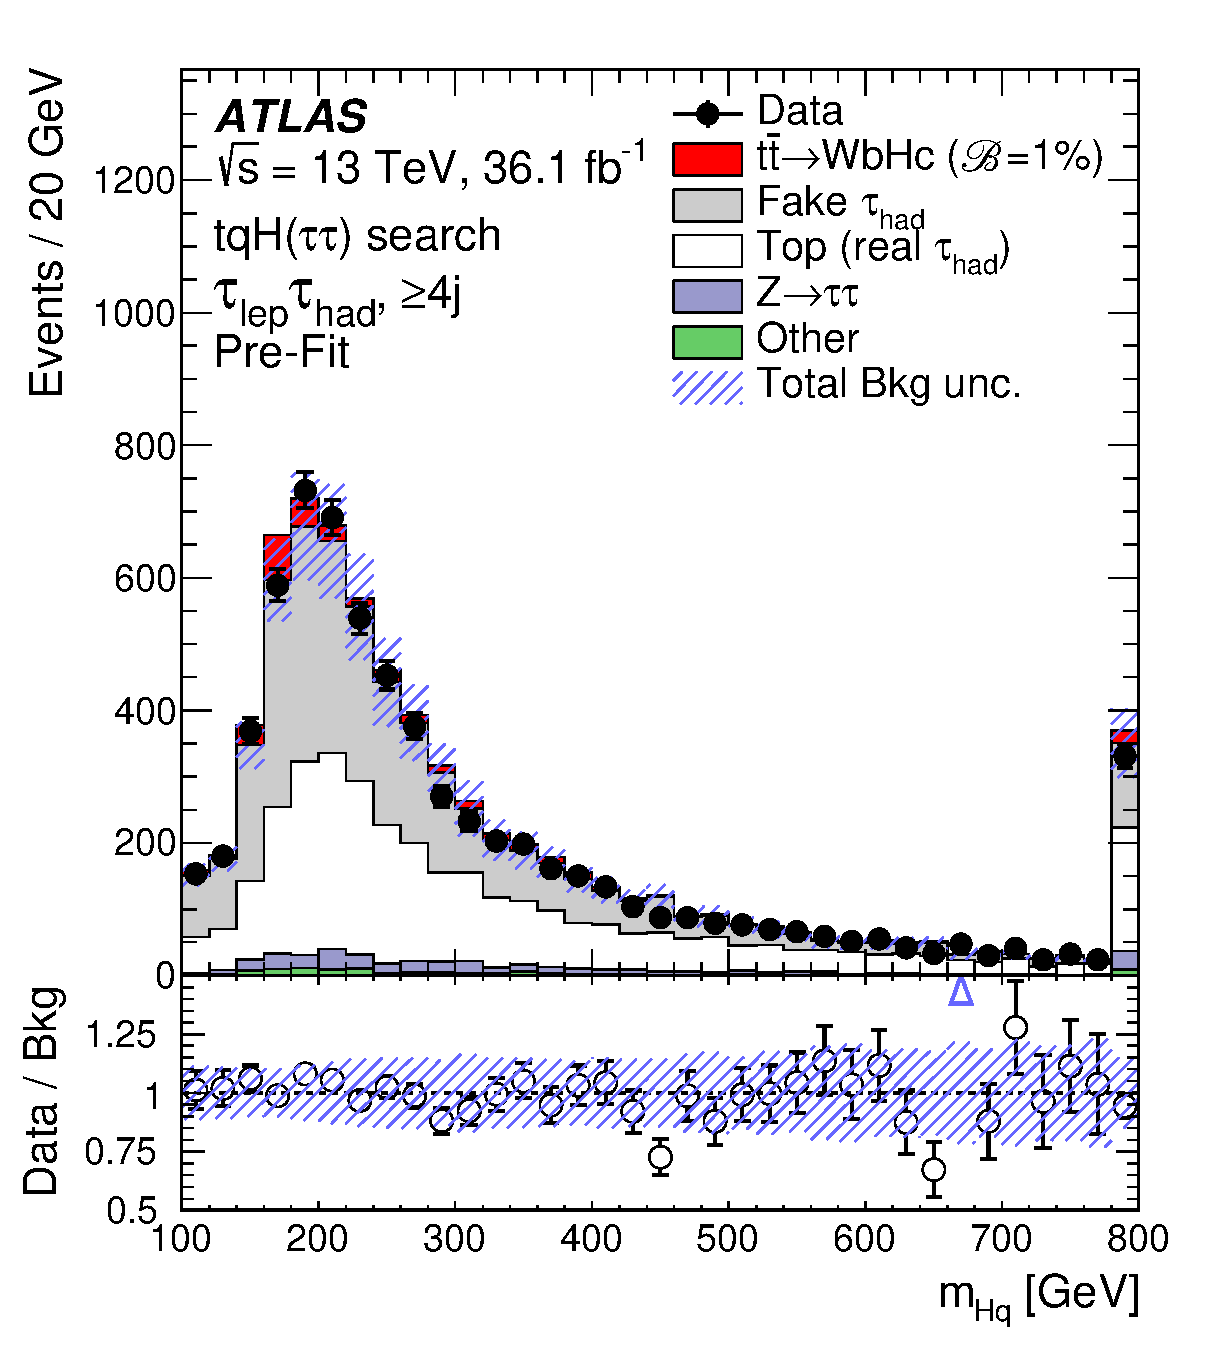
\includegraphics[width=0.40\textwidth]{figures/Htautau/control_plots/mtop_thc_lephad_4j_FR.eps}} \\
\caption{$\Htautau$ search: Comparison between the data and background prediction for the distribution of some of the most
discriminating BDT input variables in the $\lephad$ channel before the fit to data (``Pre-Fit''). The distributions are shown for
$\met$ $\phi$ centrality in (a) the ($\lephad$, 3j) region and (b) the ($\lephad$, $\geq$4j) region, and for
$m_{Hq}$ in (c) the ($\lephad$, 3j)  region and (d) the ($\lephad$, $\geq$4j) region.
The contributions with real $\had$ candidates from $\ttbar$,  $\ttbar V$, $\ttbar H$, and single top backgrounds are combined into
a single background source referred to as ``Top (real $\had$)", whereas the small contributions from 
$Z\to \ell^+\ell^-$ ($\ell = e, \mu$) and diboson backgrounds are combined into ``Other''. 
The expected $\Hc$ signal (solid red) corresponding to $\BR(t\to Hc)=1\%$ is also shown,
added to the background prediction.
%The first and the last bins in all figures contain the underflow and overflow respectively.
The bottom panel displays the ratio of data to the SM background (``Bkg'') prediction.
The hashed area represents the total uncertainty of the background, excluding the normalisation uncertainty of the fake $\had$ background, 
which is determined via a likelihood fit to data.}
\label{fig:BDT_inputs_lephad_3}
\end{center}
\end{figure*}
%%%%%%%%%%%%%%%%%%%%%%%%%%%%%%%%%%%%%%%


%%%%%%%%%%%%%%%%%%%%%%%%%%%%%%%%%%%%%%%
\begin{figure*}[t]
\begin{center}
\subfloat[]{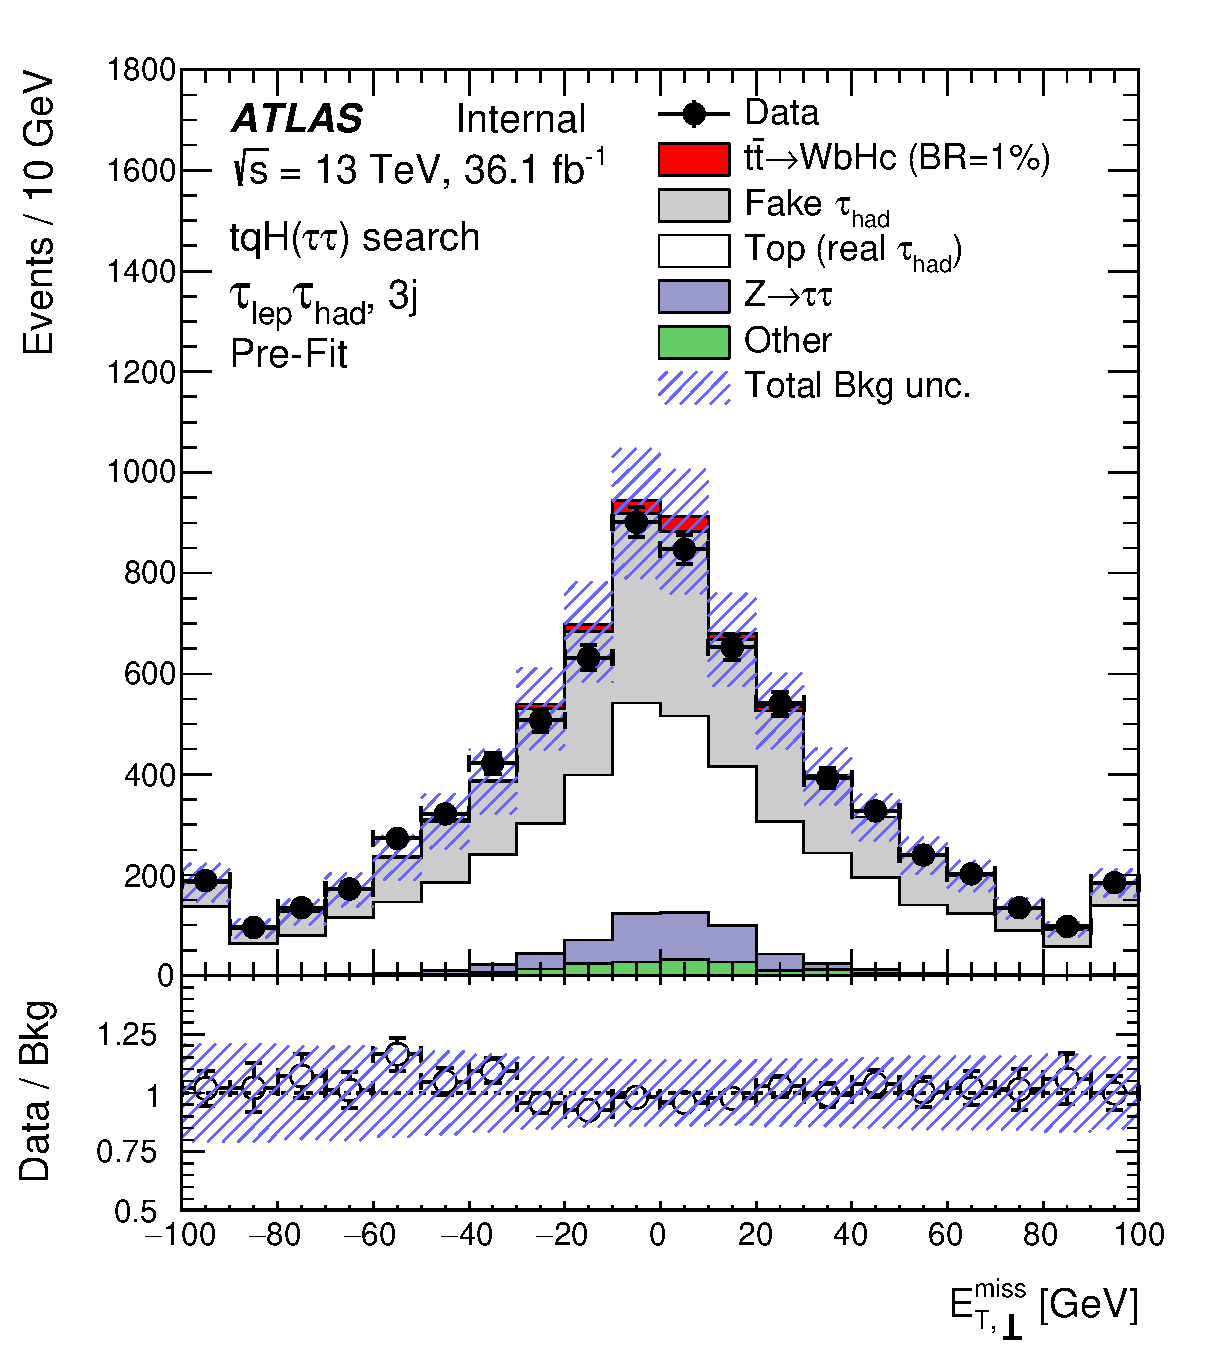
\includegraphics[width=0.40\textwidth]{figures/Htautau/control_plots/MET_perp_lephad_3j_FR.eps}}
\subfloat[]{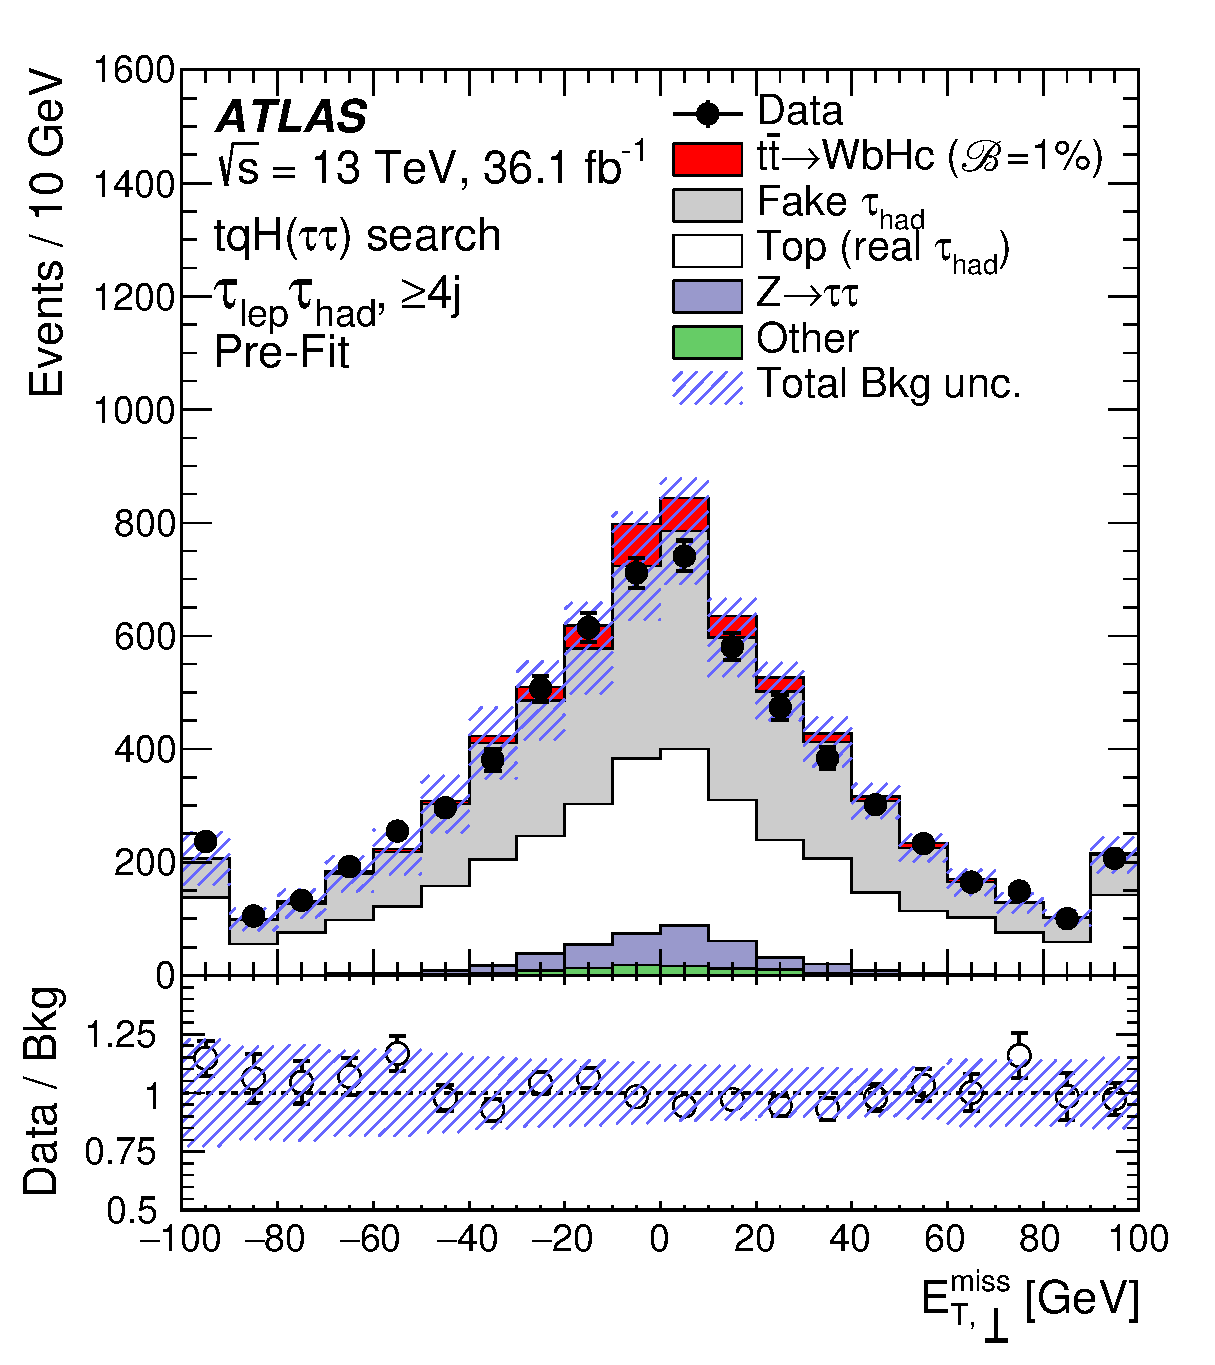
\includegraphics[width=0.40\textwidth]{figures/Htautau/control_plots/MET_perp_lephad_4j_FR.eps}} \\
\subfloat[]{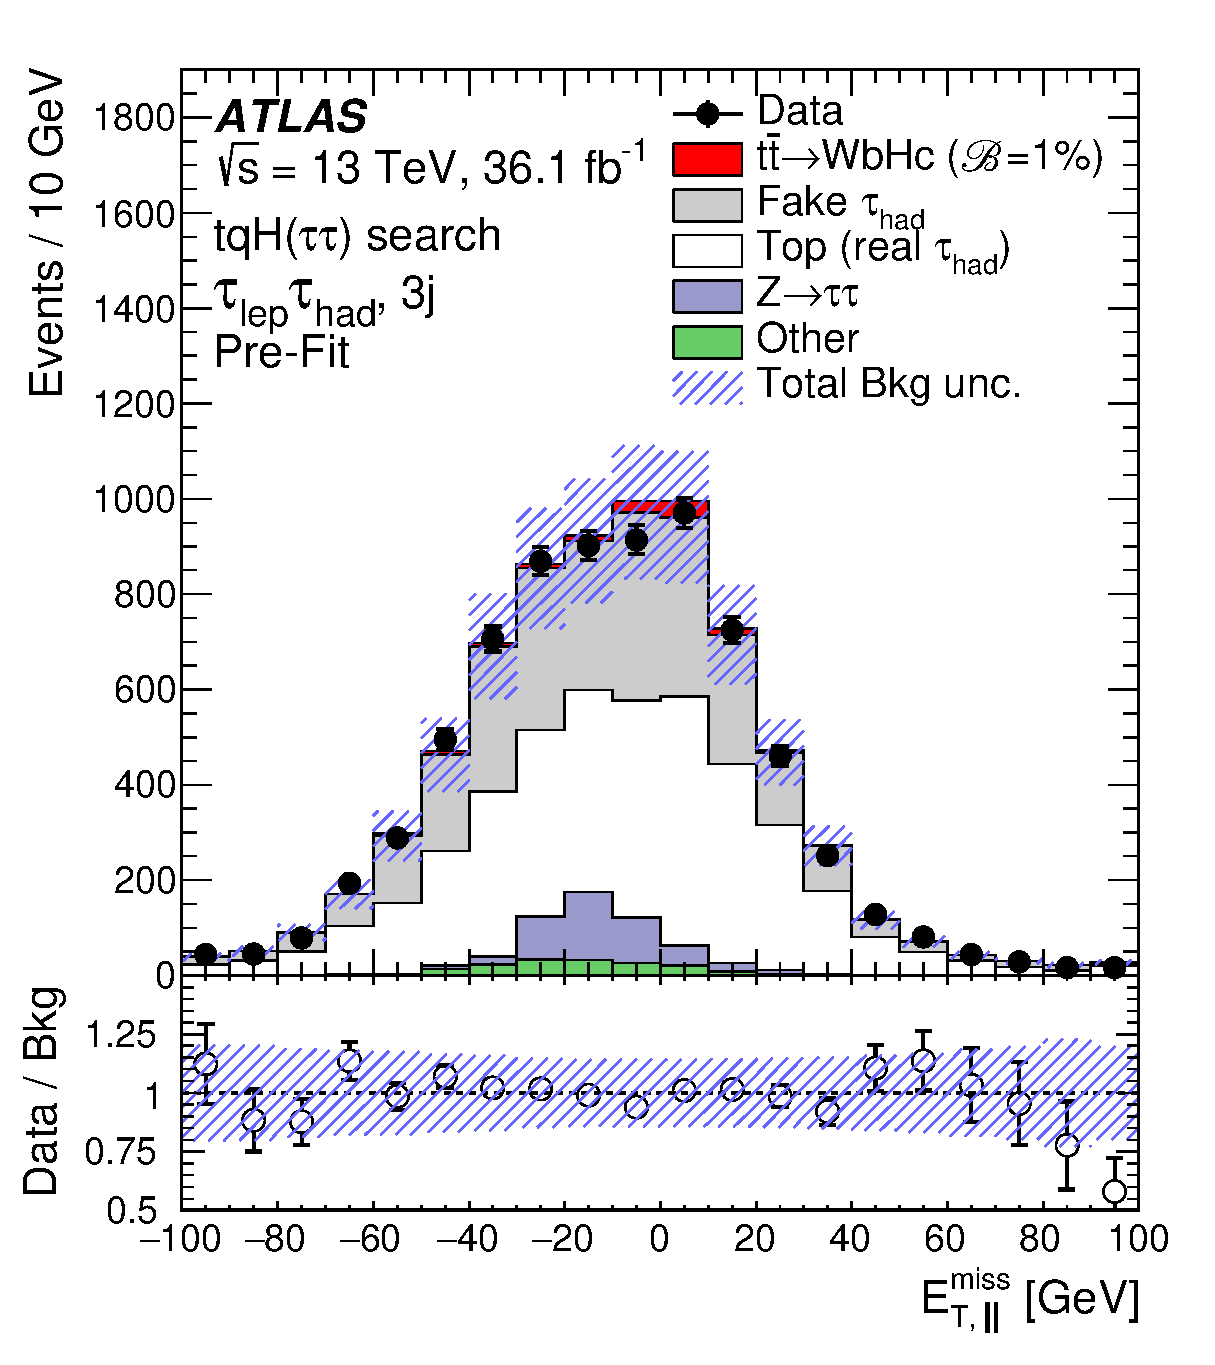
\includegraphics[width=0.40\textwidth]{figures/Htautau/control_plots/MET_proj_lephad_3j_FR.eps}}
\subfloat[]{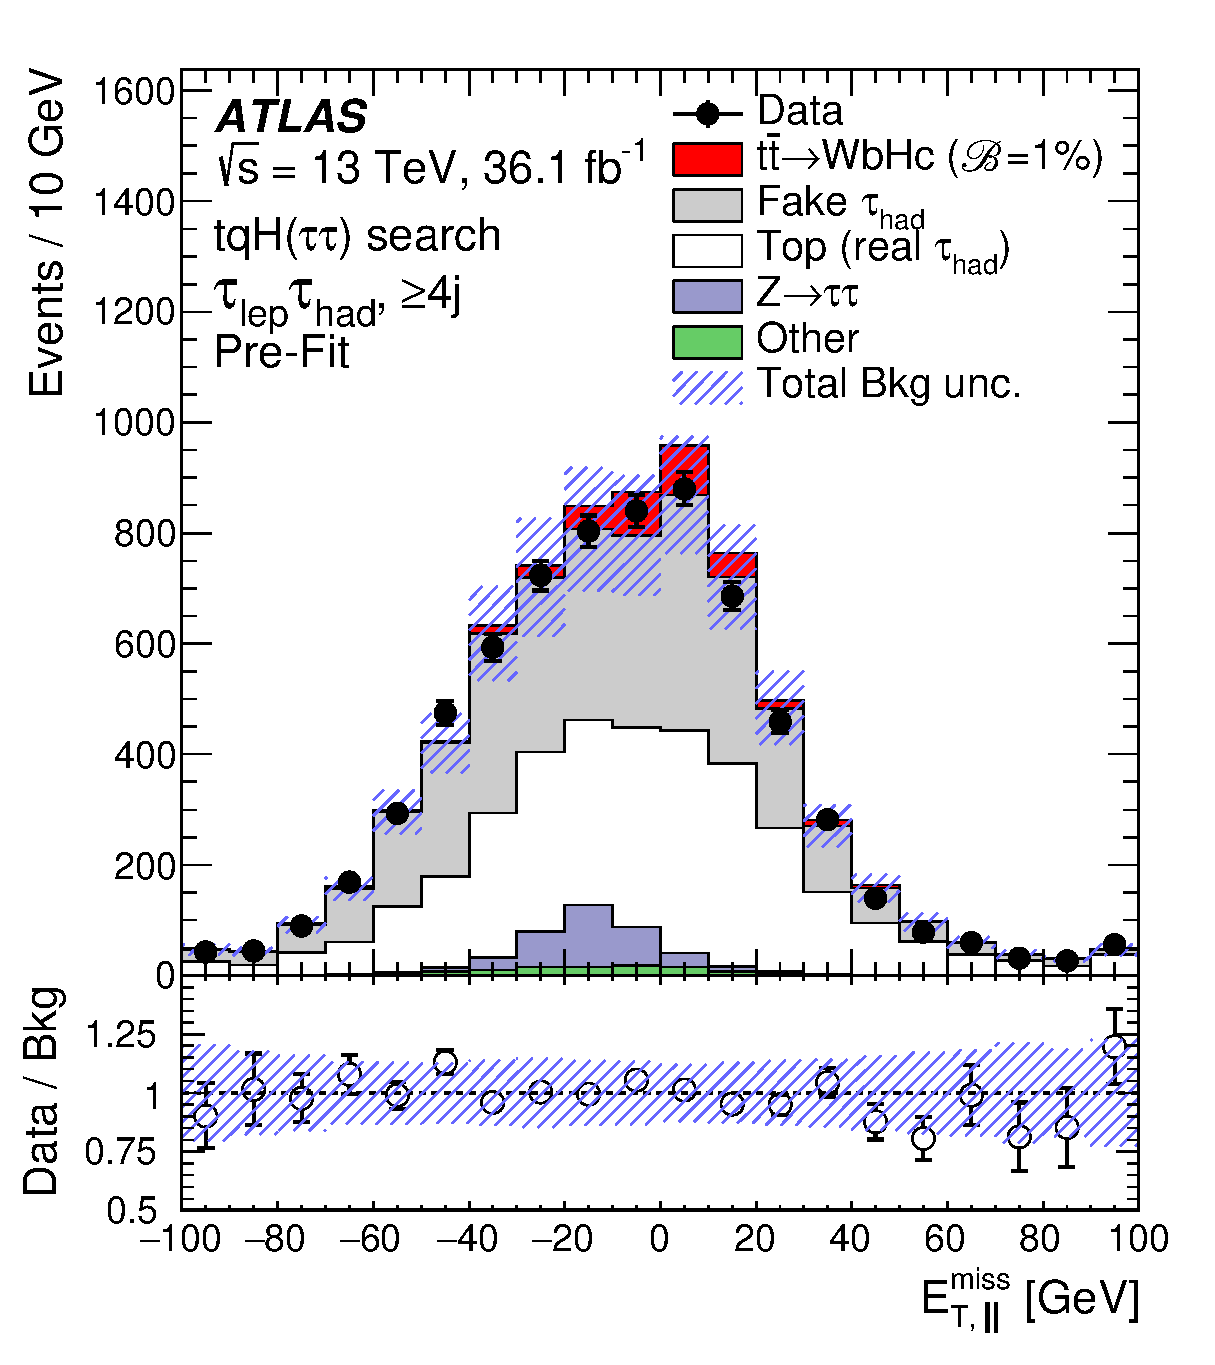
\includegraphics[width=0.40\textwidth]{figures/Htautau/control_plots/MET_proj_lephad_4j_FR.eps}} \\
\caption{$\Htautau$ search: Comparison between the data and background prediction for the distribution of some of the most
discriminating BDT input variables in the $\lephad$ channel before the fit to data (``Pre-Fit''). The distributions are shown for
$E_{\text{T},\perp}^{\text{miss}}$ in (a) the ($\lephad$, 3j) region and (b) the ($\lephad$, $\geq$4j) region, and for
$E_{\text{T},\parallel}^{\text{miss}}$ in (c) the ($\lephad$, 3j)  region and (d) the ($\lephad$, $\geq$4j) region.
The contributions with real $\had$ candidates from $\ttbar$,  $\ttbar V$, $\ttbar H$, and single top backgrounds are combined into
a single background source referred to as ``Top (real $\had$)", whereas the small contributions from 
$Z\to \ell^+\ell^-$ ($\ell = e, \mu$) and diboson backgrounds are combined into ``Other''. 
The expected $\Hc$ signal (solid red) corresponding to $\BR(t\to Hc)=1\%$ is also shown,
added to the background prediction.
%The first and the last bins in all figures contain the underflow and overflow respectively.
The bottom panel displays the ratio of data to the SM background (``Bkg'') prediction.
The hashed area represents the total uncertainty of the background, excluding the normalisation uncertainty of the fake $\had$ background, 
which is determined via a likelihood fit to data.}
\label{fig:BDT_inputs_lephad_4}
\end{center}
\end{figure*}
%%%%%%%%%%%%%%%%%%%%%%%%%%%%%%%%%%%%%%%



%%%%%%%%%%%%%%%%%%%%%%%%%%%%%%%%%%%%%%%
\begin{figure*}[t]
\begin{center}
\subfloat[]{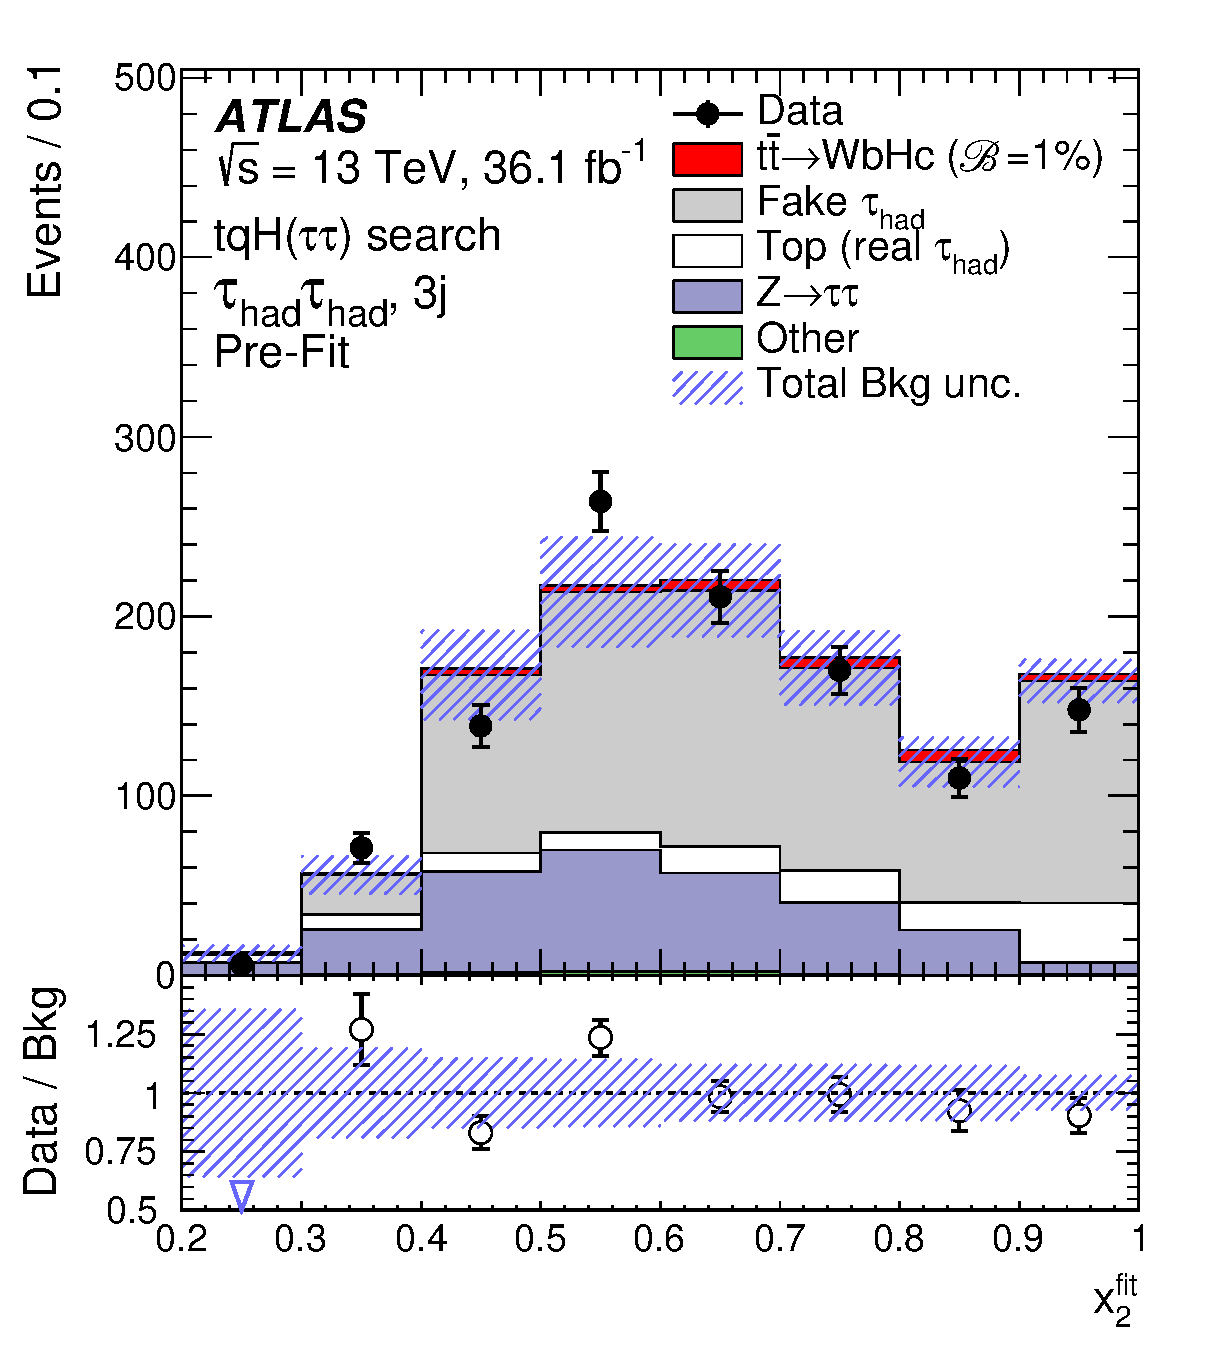
\includegraphics[width=0.40\textwidth]{figures/Htautau/control_plots/x2_fit_hadhad_3j_FR.eps}}
\subfloat[]{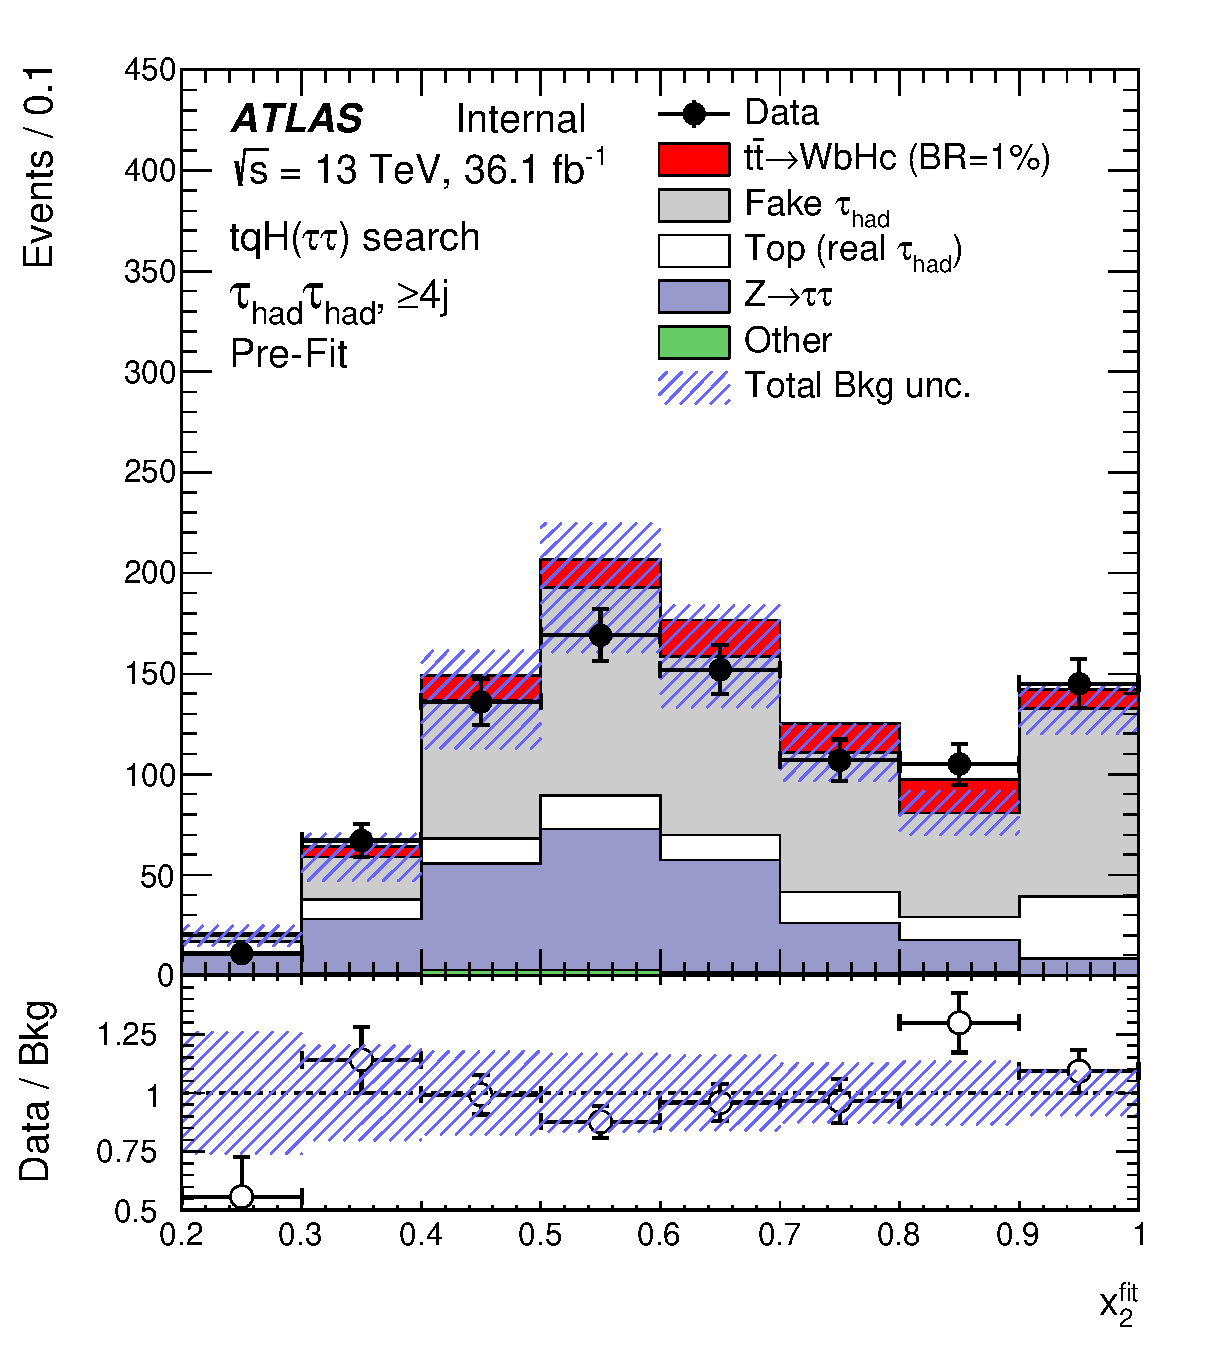
\includegraphics[width=0.40\textwidth]{figures/Htautau/control_plots/x2_fit_hadhad_4j_FR.eps}} \\
\subfloat[]{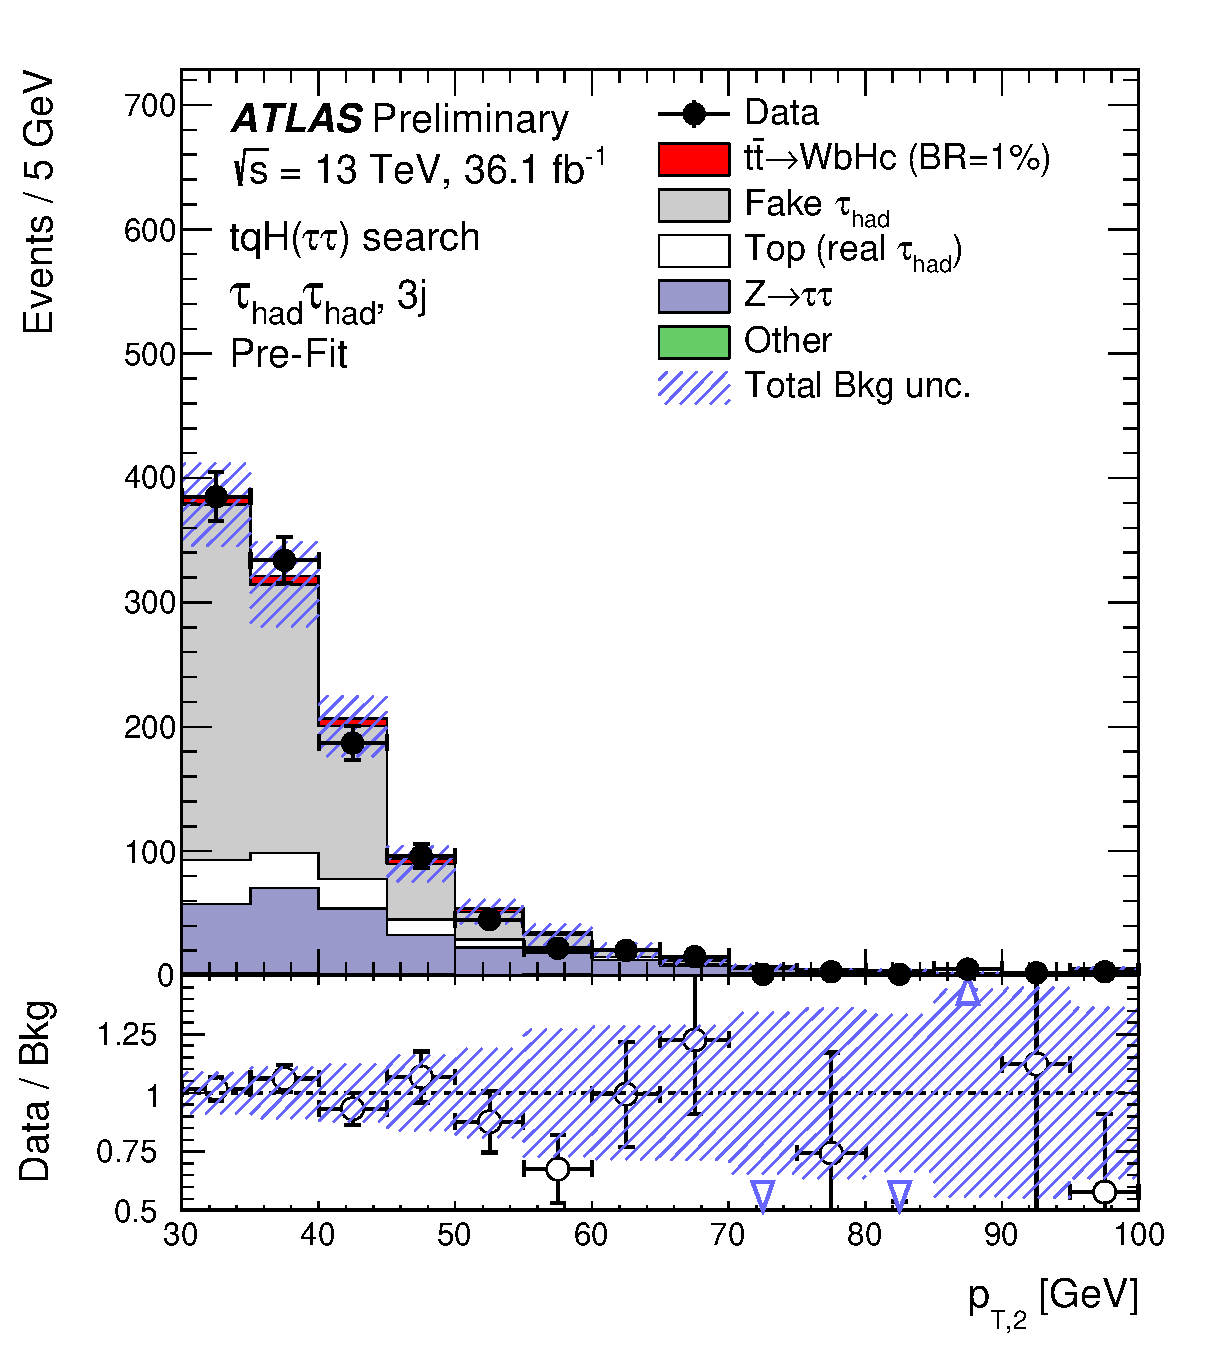
\includegraphics[width=0.40\textwidth]{figures/Htautau/control_plots/ptL2_hadhad_3j_FR.eps}}
\subfloat[]{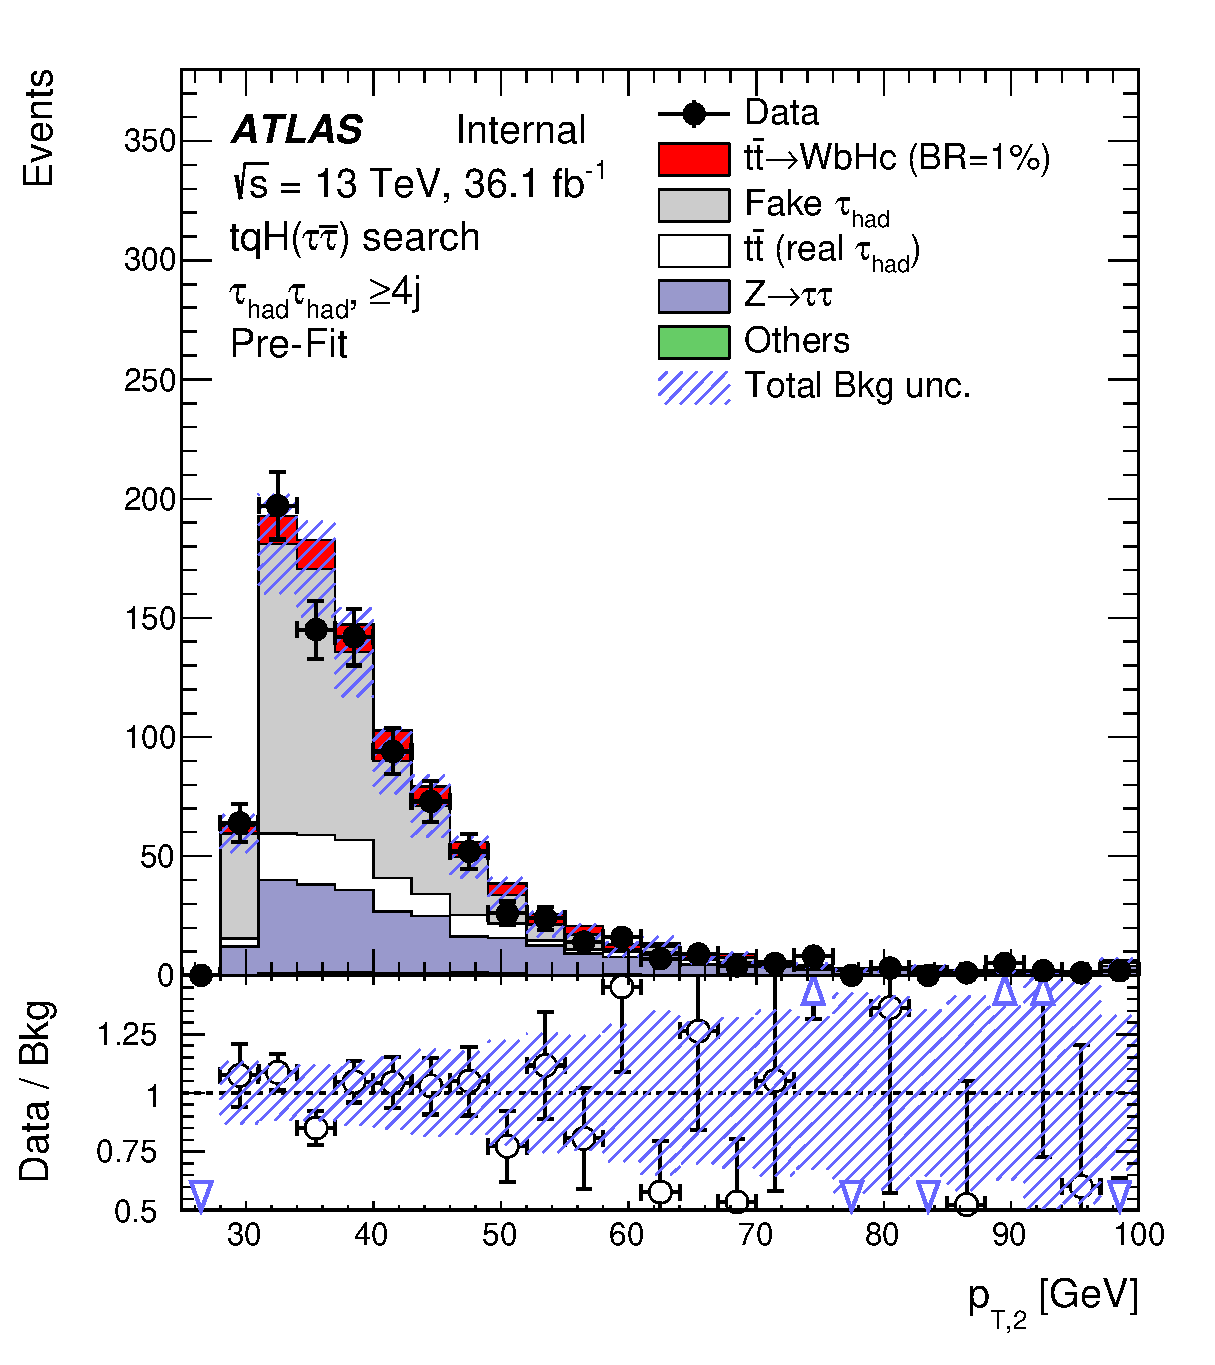
\includegraphics[width=0.40\textwidth]{figures/Htautau/control_plots/ptL2_hadhad_4j_FR.eps}} \\
\caption{$\Htautau$ search: Comparison between the data and background prediction for the distribution of two of the most 
discriminating BDT input variables in the $\hadhad$ channel before the fit to data (``Pre-Fit''). The distributions are shown for
$x_{2}^{\text{fit}}$ in (a) the ($\hadhad$, 3j) region and (b) the ($\hadhad$, $\geq$4j) region, and for
$p_{\text{T},2}$ in (c) the ($\hadhad$, 3j)  region and (d) the ($\hadhad$, $\geq$4j) region.
The contributions with real $\had$ candidates from $\ttbar$,  $\ttbar V$, $\ttbar H$, and single top backgrounds are combined into
a single background source referred to as ``Top (real $\had$)", whereas the small contributions from 
$Z\to \ell^+\ell^-$ ($\ell = e, \mu$) and diboson backgrounds are combined into ``Other''. 
The expected $\Hc$ signal (solid red) corresponding to $\BR(t\to Hc)=1\%$ is also shown,
added to the background prediction.
The first and the last bins in the figures in (c) and (d) contain the underflow and overflow respectively.
The bottom panel displays the ratio of data to the SM background (``Bkg'') prediction.
The hashed area represents the total uncertainty of the background, excluding the normalisation uncertainty of the fake $\had$ background, 
which is determined via a likelihood fit to data.} 
\label{fig:BDT_inputs_hadhad_2}
\end{center}
\end{figure*}
%%%%%%%%%%%%%%%%%%%%%%%%%%%%%%%%%%%%%%%

%%%%%%%%%%%%%%%%%%%%%%%%%%%%%%%%%%%%%%%
\begin{figure*}[t]
\begin{center}
\subfloat[]{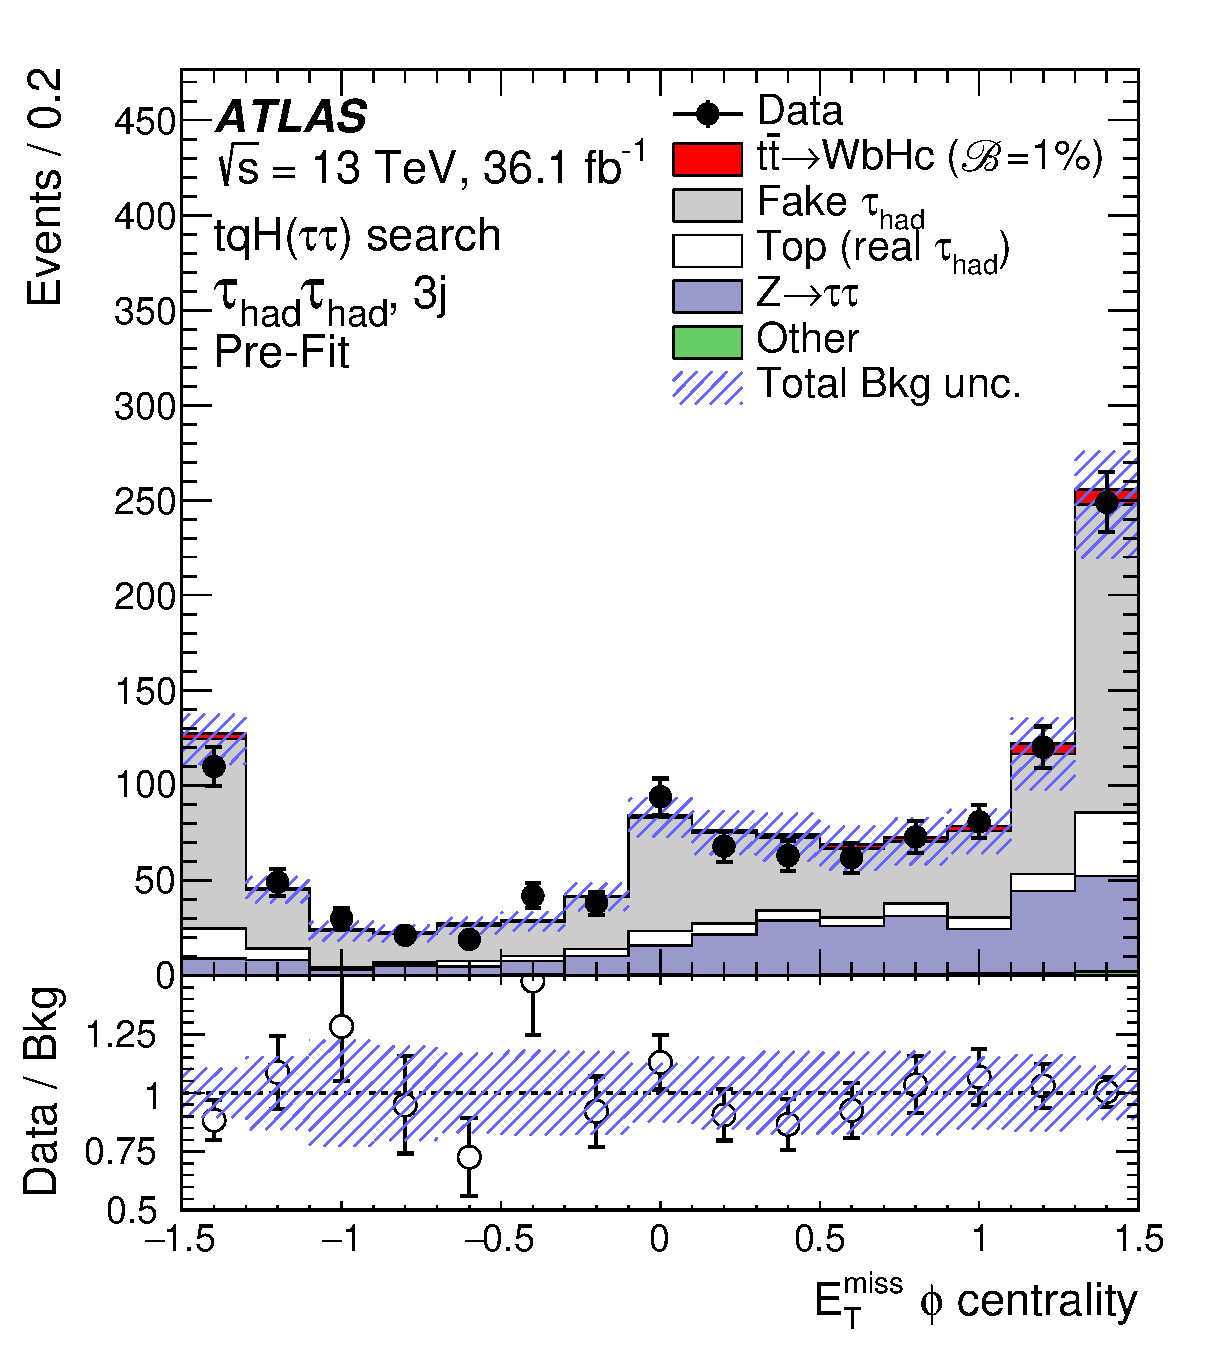
\includegraphics[width=0.40\textwidth]{figures/Htautau/control_plots/met_centrality_hadhad_3j_FR.eps}}
\subfloat[]{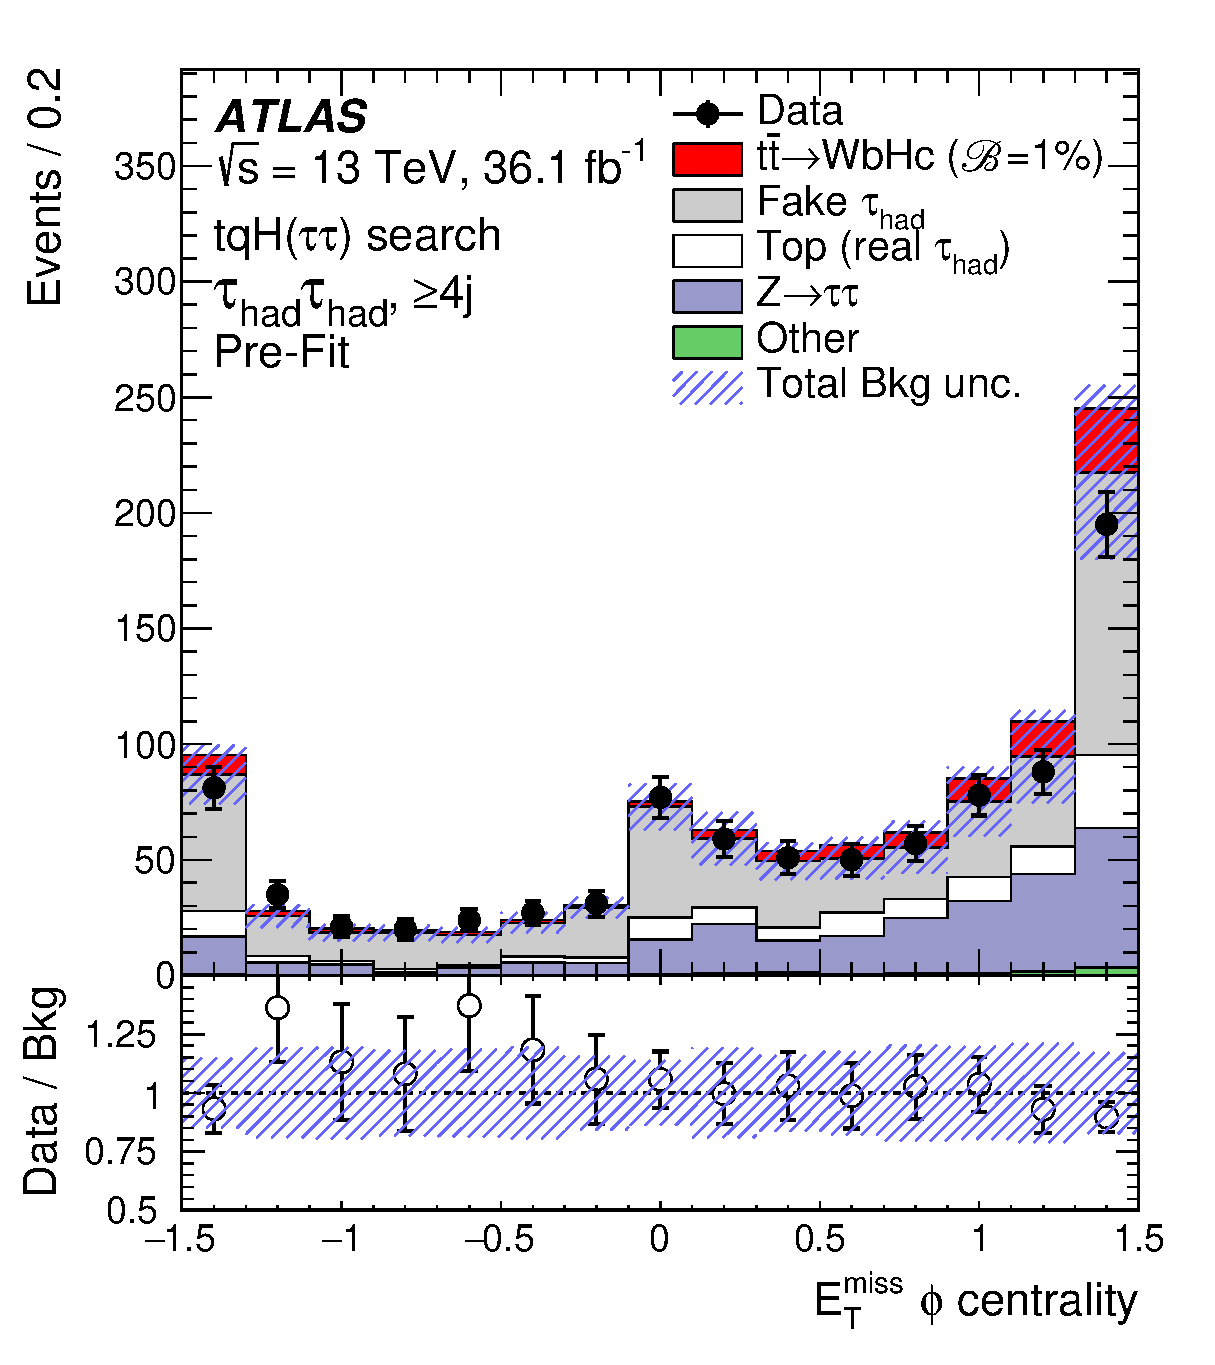
\includegraphics[width=0.40\textwidth]{figures/Htautau/control_plots/met_centrality_hadhad_4j_FR.eps}} \\
\subfloat[]{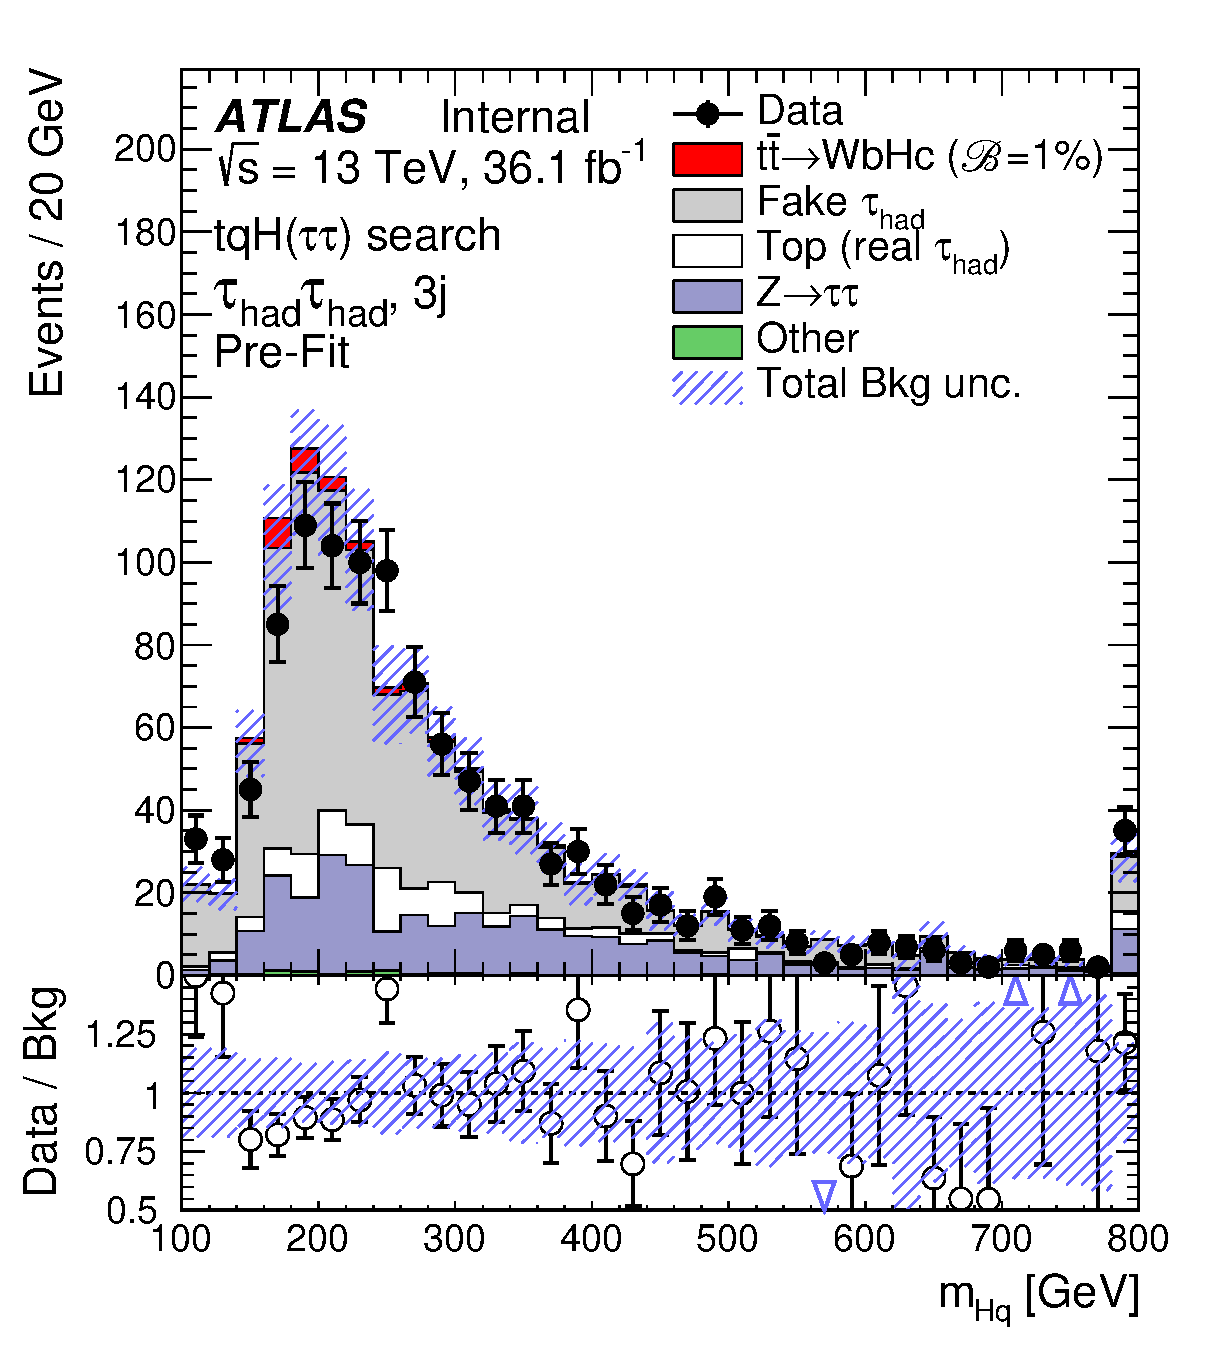
\includegraphics[width=0.40\textwidth]{figures/Htautau/control_plots/mtop_thc_hadhad_3j_FR.eps}}
\subfloat[]{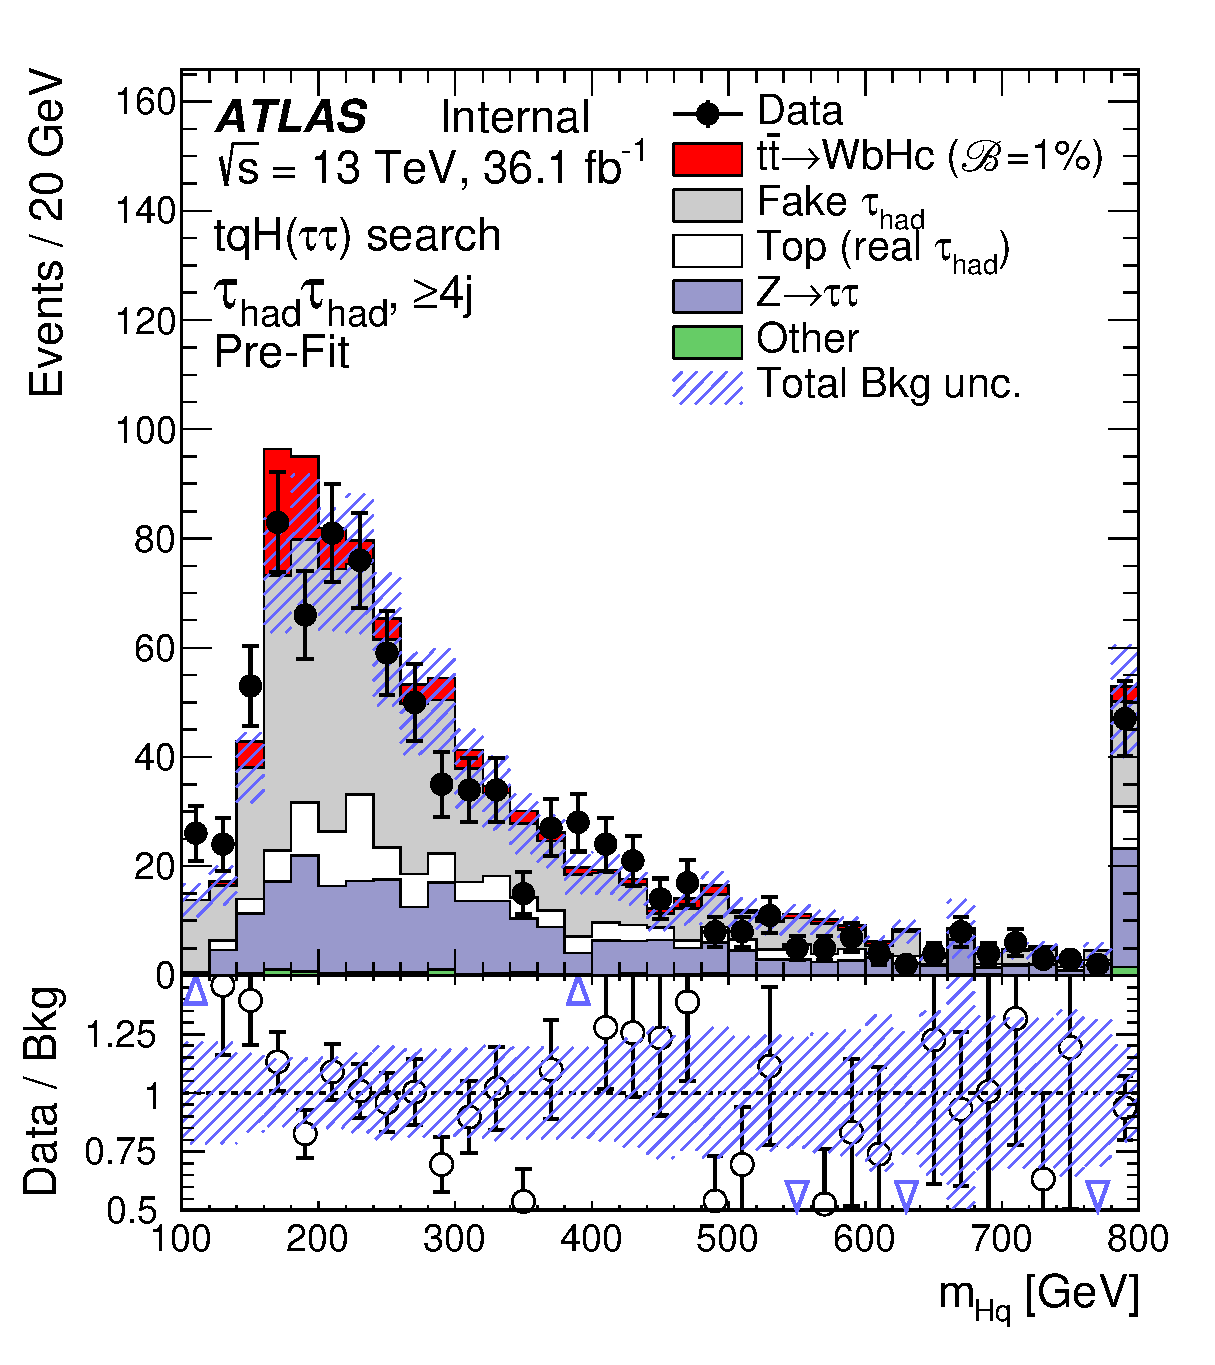
\includegraphics[width=0.40\textwidth]{figures/Htautau/control_plots/mtop_thc_hadhad_4j_FR.eps}} \\
\caption{$\Htautau$ search: Comparison between the data and background prediction for the distribution of two of the most 
discriminating BDT input variables in the $\hadhad$ channel before the fit to data (``Pre-Fit''). The distributions are shown for
$\met$ $\phi$ centrality  in (a) the ($\hadhad$, 3j) region and (b) the ($\hadhad$, $\geq$4j) region, and for
$m_{Hq}$ in (c) the ($\hadhad$, 3j)  region and (d) the ($\hadhad$, $\geq$4j) region.
The contributions with real $\had$ candidates from $\ttbar$,  $\ttbar V$, $\ttbar H$, and single top backgrounds are combined into
a single background source referred to as ``Top (real $\had$)", whereas the small contributions from 
$Z\to \ell^+\ell^-$ ($\ell = e, \mu$) and diboson backgrounds are combined into ``Other''. 
The expected $\Hc$ signal (solid red) corresponding to $\BR(t\to Hc)=1\%$ is also shown,
added to the background prediction.
The first and the last bins in the figures in (c) and (d) contain the underflow and overflow respectively.
The bottom panel displays the ratio of data to the SM background (``Bkg'') prediction.
The hashed area represents the total uncertainty of the background, excluding the normalisation uncertainty of the fake $\had$ background, 
which is determined via a likelihood fit to data.} 
\label{fig:BDT_inputs_hadhad_3}
\end{center}
\end{figure*}
%%%%%%%%%%%%%%%%%%%%%%%%%%%%%%%%%%%%%%%


%%%%%%%%%%%%%%%%%%%%%%%%%%%%%%%%%%%%%%%
\begin{figure*}[t]
\begin{center}
\subfloat[]{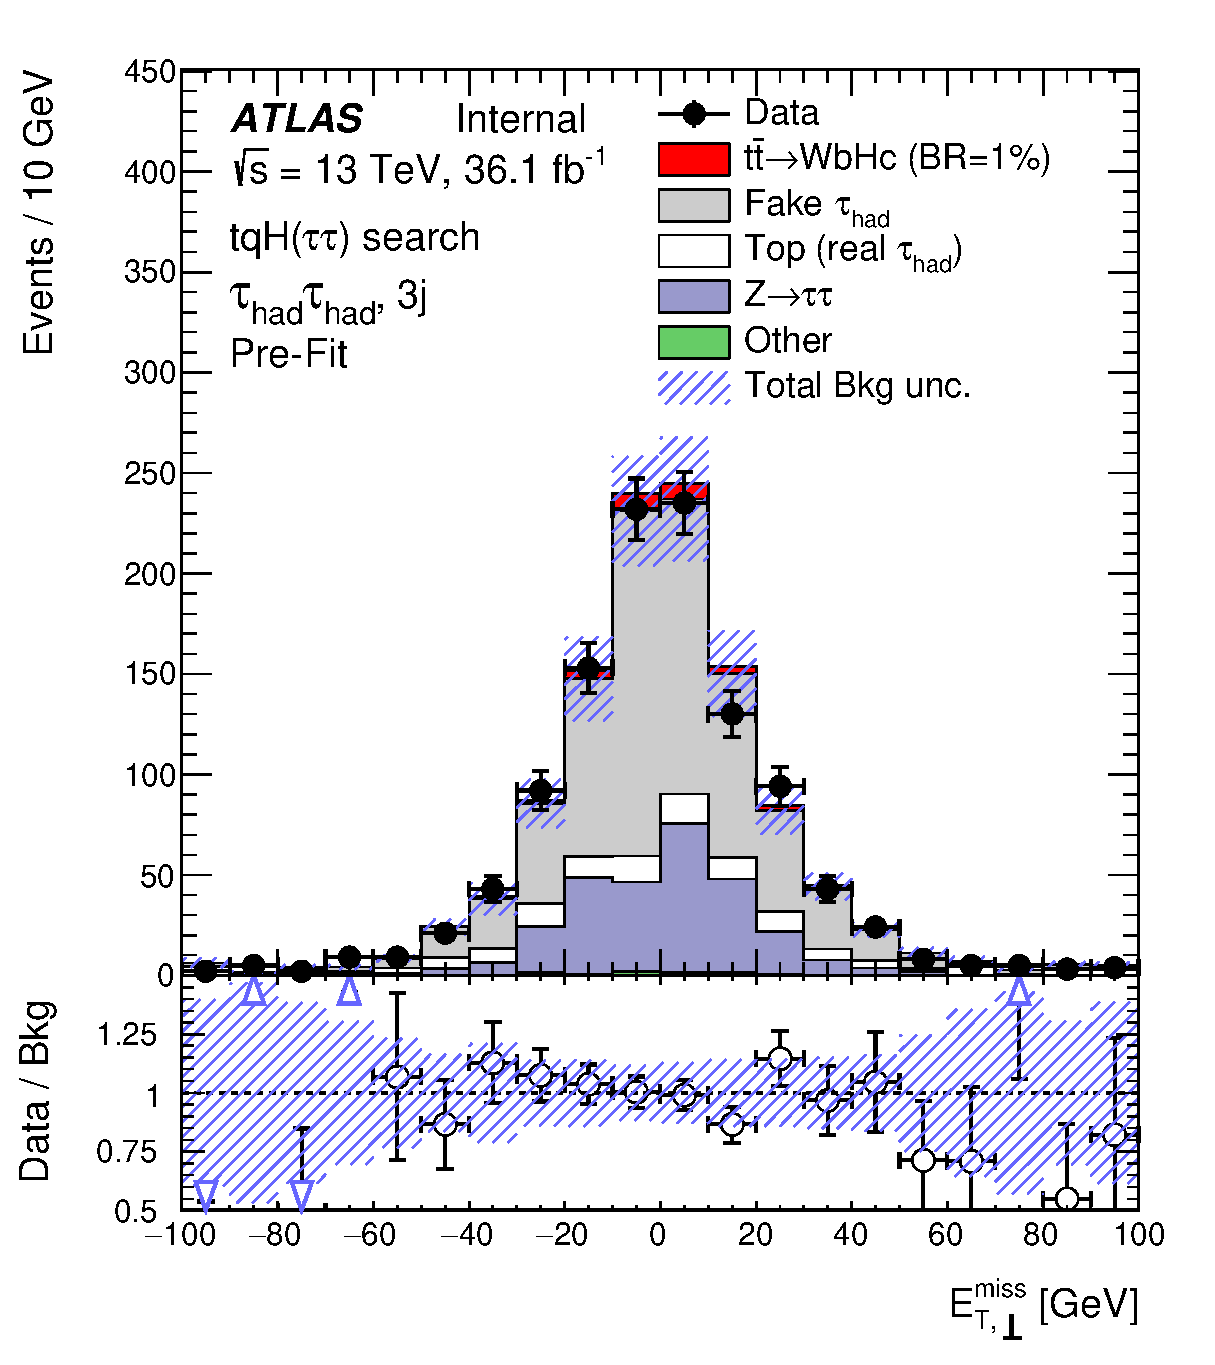
\includegraphics[width=0.40\textwidth]{figures/Htautau/control_plots/MET_perp_hadhad_3j_FR.eps}}
\subfloat[]{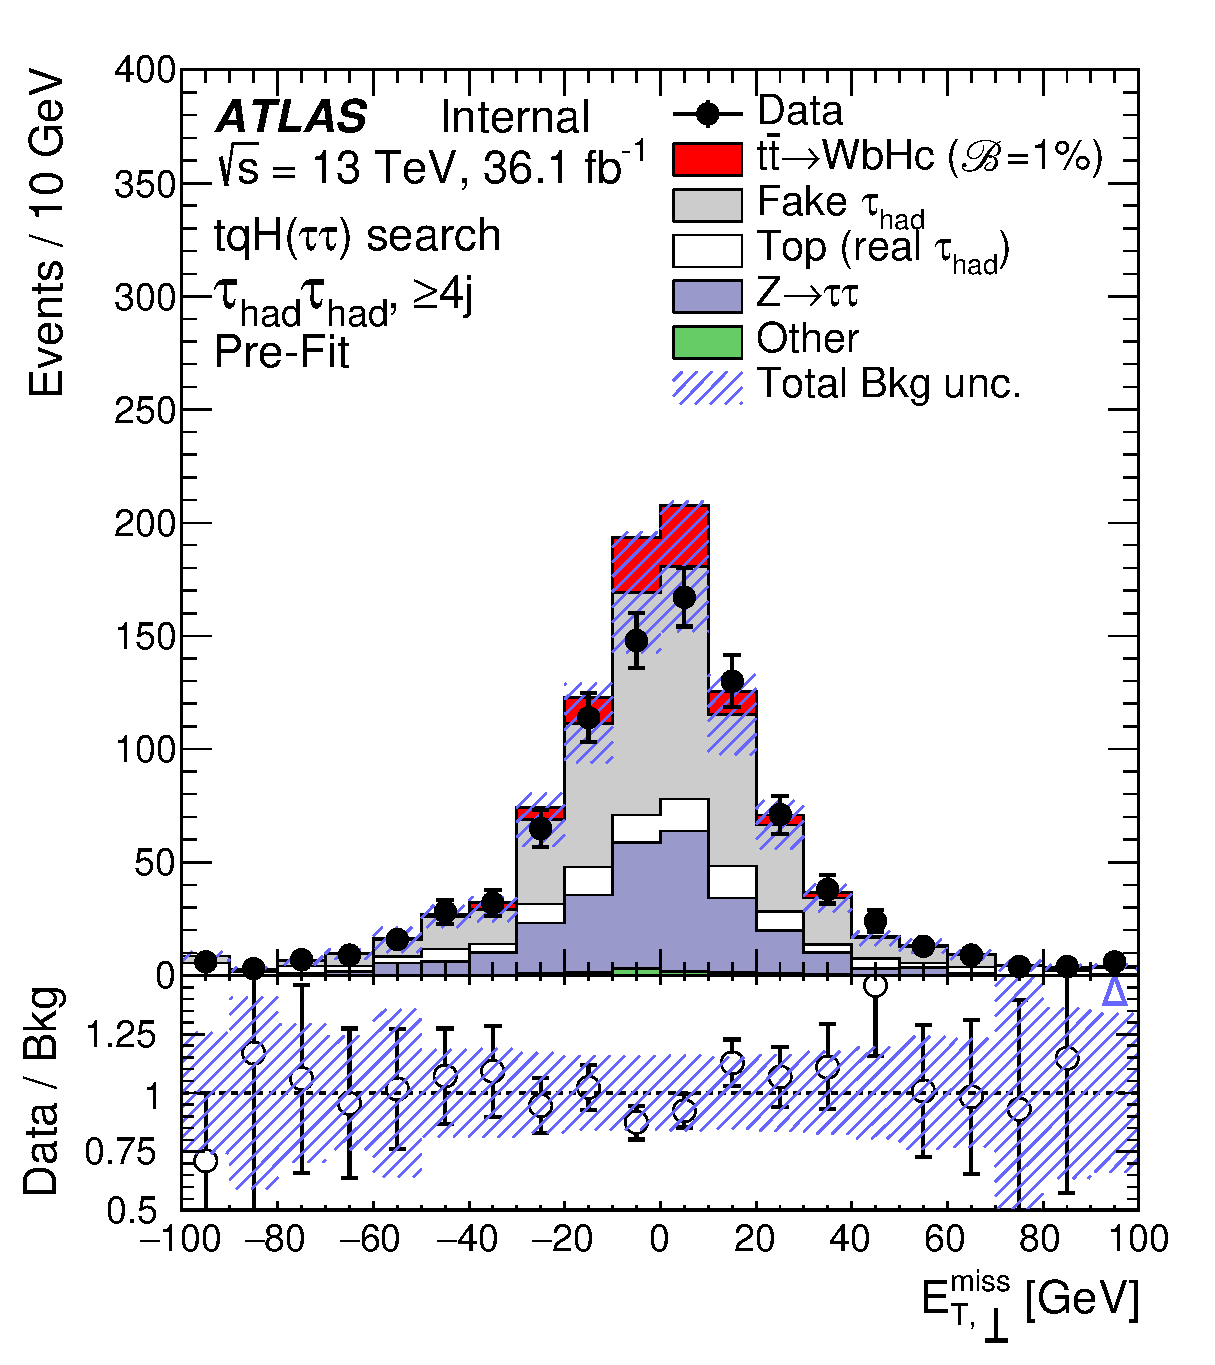
\includegraphics[width=0.40\textwidth]{figures/Htautau/control_plots/MET_perp_hadhad_4j_FR.eps}} \\
\subfloat[]{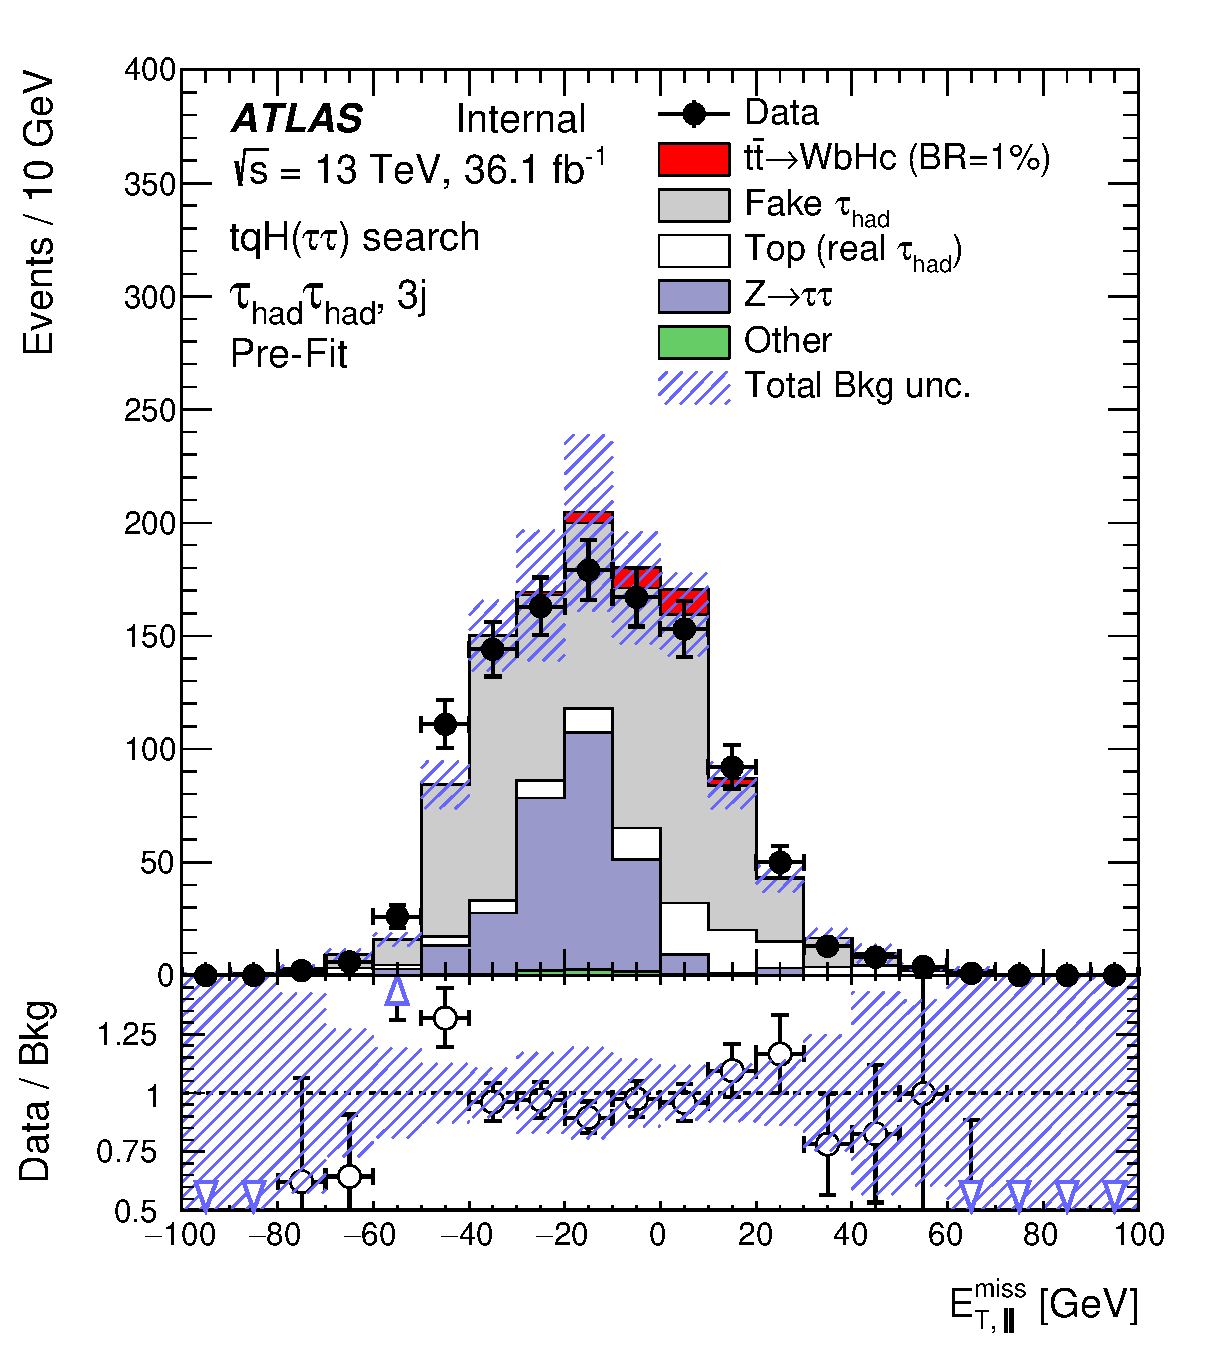
\includegraphics[width=0.40\textwidth]{figures/Htautau/control_plots/MET_proj_hadhad_3j_FR.eps}}
\subfloat[]{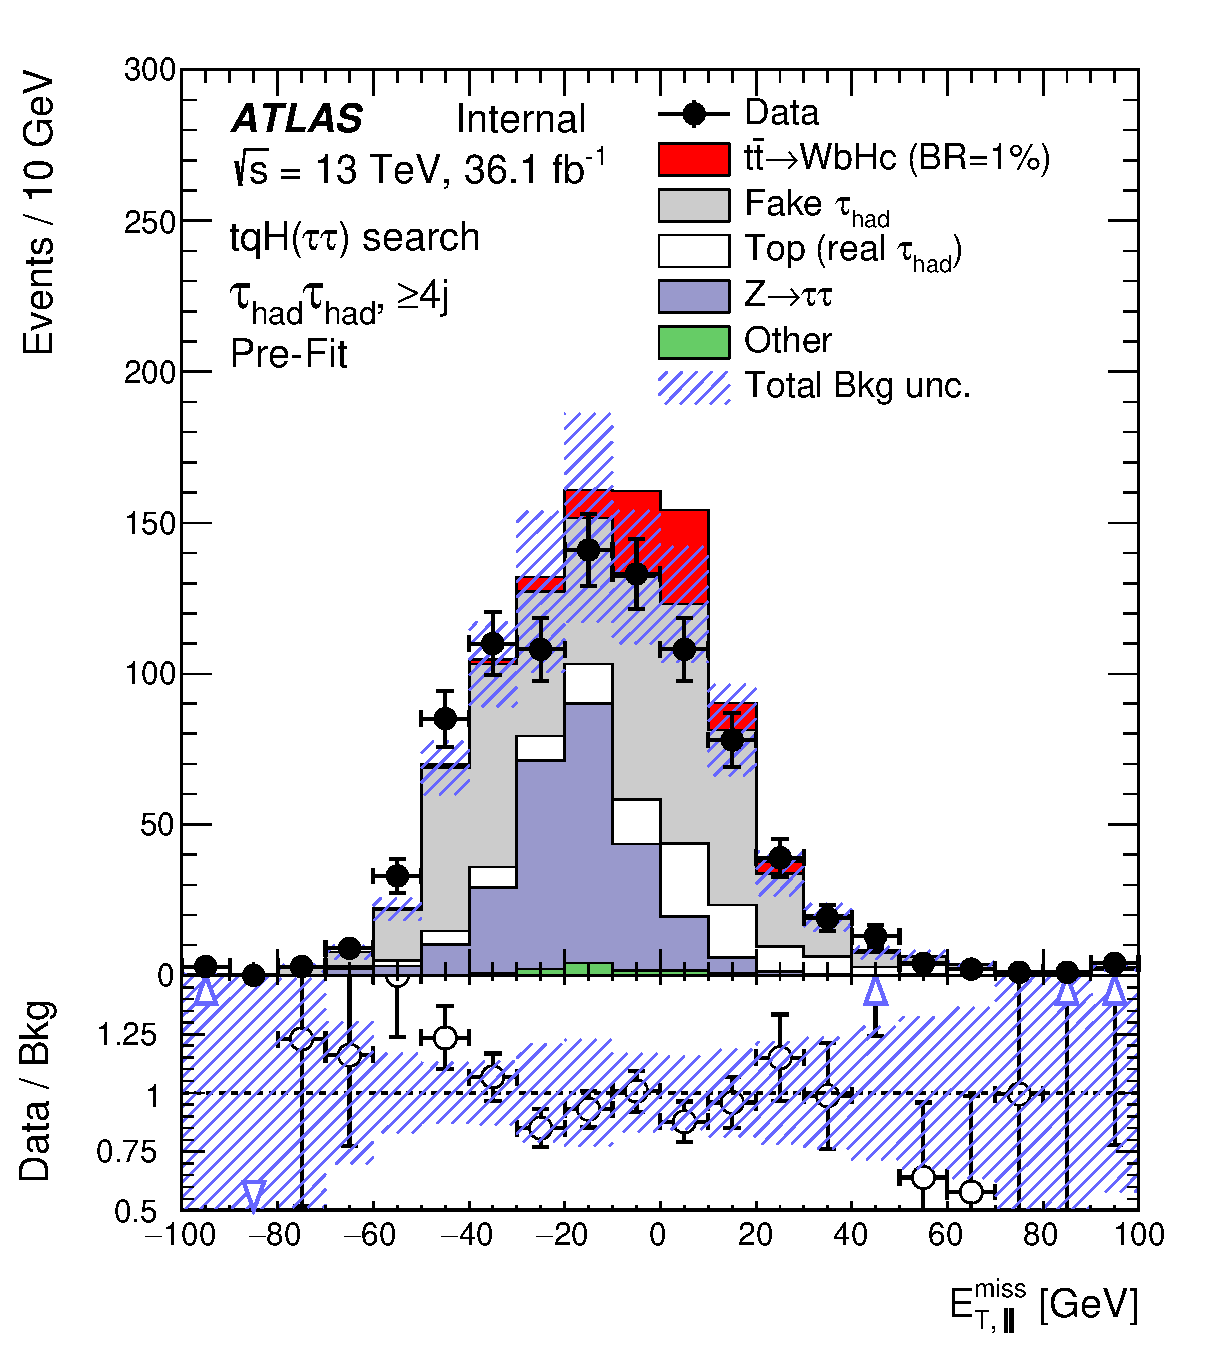
\includegraphics[width=0.40\textwidth]{figures/Htautau/control_plots/MET_proj_hadhad_4j_FR.eps}} \\
\caption{$\Htautau$ search: Comparison between the data and background prediction for the distribution of two of the most 
discriminating BDT input variables in the $\hadhad$ channel before the fit to data (``Pre-Fit''). The distributions are shown for
$E_{\text{T},\perp}^{\text{miss}}$ in (a) the ($\hadhad$, 3j) region and (b) the ($\hadhad$, $\geq$4j) region, and for
$E_{\text{T},\parallel}^{\text{miss}}$ in (c) the ($\hadhad$, 3j)  region and (d) the ($\hadhad$, $\geq$4j) region.
The contributions with real $\had$ candidates from $\ttbar$,  $\ttbar V$, $\ttbar H$, and single top backgrounds are combined into
a single background source referred to as ``Top (real $\had$)", whereas the small contributions from 
$Z\to \ell^+\ell^-$ ($\ell = e, \mu$) and diboson backgrounds are combined into ``Other''. 
The expected $\Hc$ signal (solid red) corresponding to $\BR(t\to Hc)=1\%$ is also shown,
added to the background prediction.
The first and the last bins in the figures in (c) and (d) contain the underflow and overflow respectively.
The bottom panel displays the ratio of data to the SM background (``Bkg'') prediction.
The hashed area represents the total uncertainty of the background, excluding the normalisation uncertainty of the fake $\had$ background, 
which is determined via a likelihood fit to data.} 
\label{fig:BDT_inputs_hadhad_4}
\end{center}
\end{figure*}
%%%%%%%%%%%%%%%%%%%%%%%%%%%%%%%%%%%%%%%


%%%%%%%%%%%%%%%%%%%%%%%%%%%%%%%%%%%%%%%
%\begin{figure*}[t]
%\begin{center}
%\subfloat[]{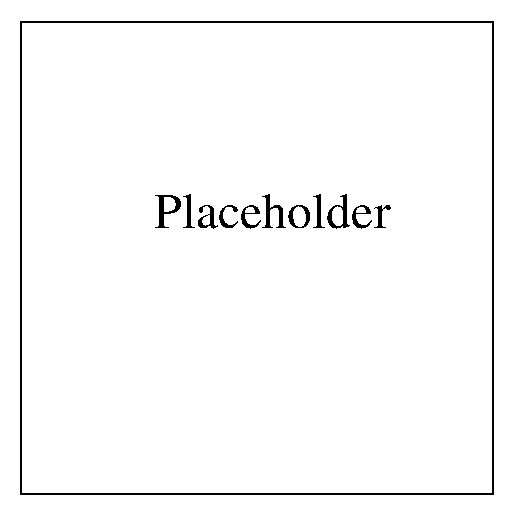
\includegraphics[width=0.40\textwidth]{figures/placeholder8x8.eps}}
%\subfloat[]{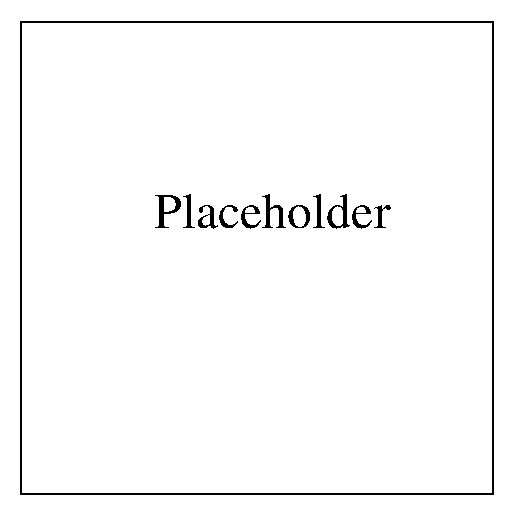
\includegraphics[width=0.40\textwidth]{figures/placeholder8x8.eps}} \\
%\subfloat[]{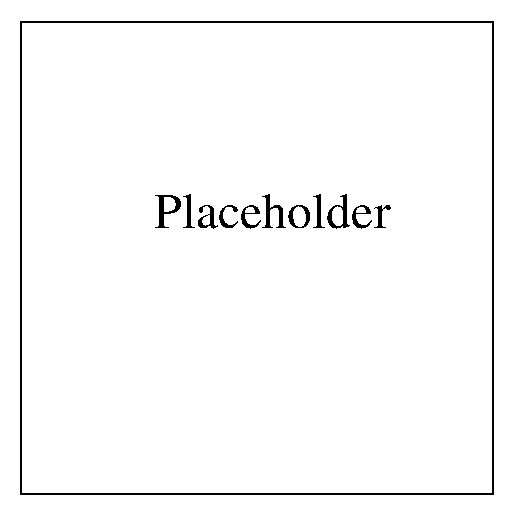
\includegraphics[width=0.40\textwidth]{figures/placeholder8x8.eps}}
%\subfloat[]{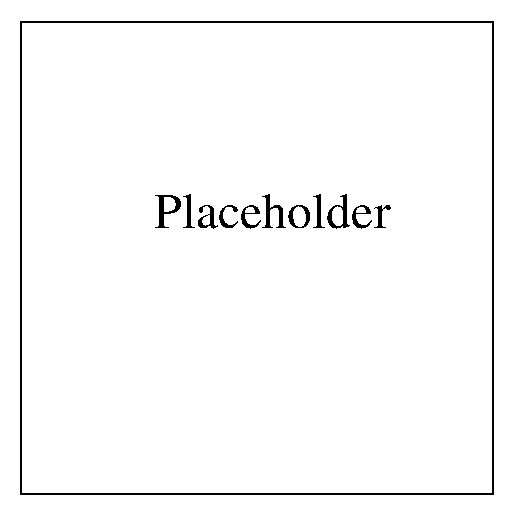
\includegraphics[width=0.40\textwidth]{figures/placeholder8x8.eps}} \\
%\caption{$\Htautau$ search: Comparison between the data and background prediction for the distribution of two of the most 
%important BDT input variables in the $\hadhad$ channel before performing the fit to data (``Pre-Fit''). The distributions are shown for
%$x_{2}^{\text{fit}}$ in (a) the ($\hadhad$, 3j) region and (b) the ($\hadhad$, $\geq$4j) region, and for
%$p_{\text{T},2}$ in (c) the ($\hadhad$, 3j)  region and (d) the ($\hadhad$, $\geq$4j) region.
%The contributions with real $\had$ candidates from $\ttbar$,  $\ttbar V$, $\ttbar H$, and single top backgrounds are combined into
%a single background source referred to as ``Top (real $\had$)", whereas the small contributions from 
%$Z\to \ell^+\ell^-$ ($\ell = e, \mu$) and diboson backgrounds are combined into ``Other''. 
%The expected $\Hc$ signal (solid red) corresponding to $\BR(t\to Hc)=1\%$ is also shown,
%added on top of the background prediction.
%The first and the last bins in the figures in (c) and (d) contain the underflow and overflow respectively.
%The bottom panel displays the ratio of data to the SM background (``Bkg'') prediction.
%The hashed area represents the total uncertainty on the background, excluding the normalisation uncertainty of the fake $\had$ background, 
%which is determined via a likelihood fit to data.} 
%\label{fig:BDT_inputs_hadhad_3}
%\end{center}
%\end{figure*}
%%%%%%%%%%%%%%%%%%%%%%%%%%%%%%%%%%%%%%%


%%%%%%%%%%%%%%%%%%%%%%%%%%%%%%%%%%%%%%%
%\begin{figure*}[t]
%\begin{center}
%\subfloat[]{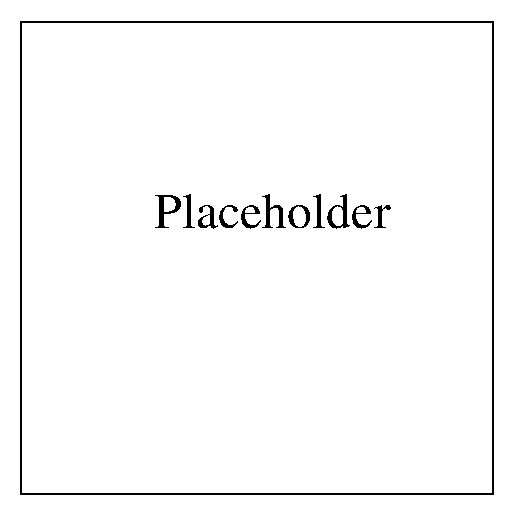
\includegraphics[width=0.40\textwidth]{figures/placeholder8x8.eps}}
%\subfloat[]{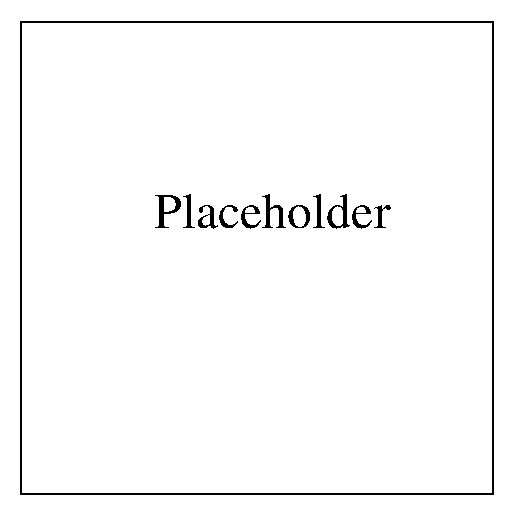
\includegraphics[width=0.40\textwidth]{figures/placeholder8x8.eps}} \\
%\subfloat[]{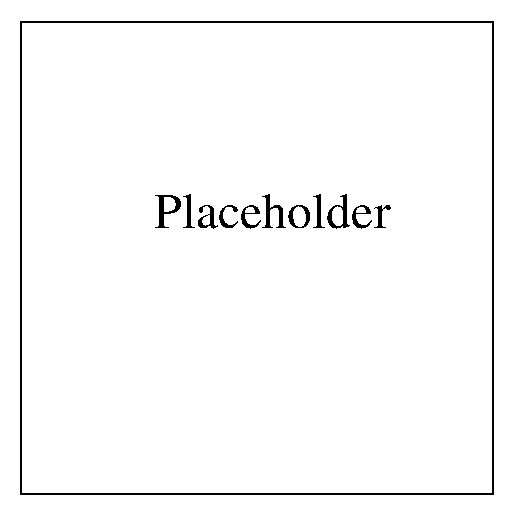
\includegraphics[width=0.40\textwidth]{figures/placeholder8x8.eps}}
%\subfloat[]{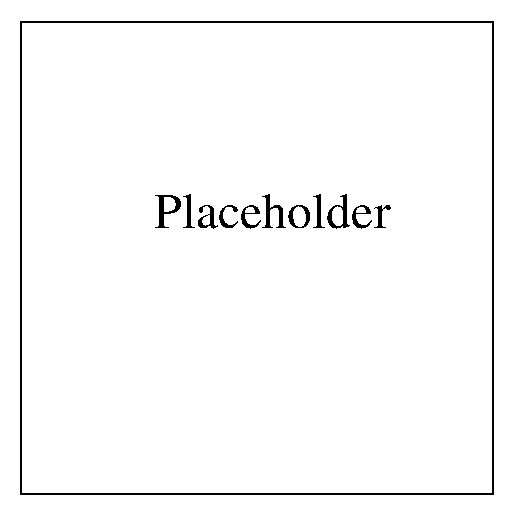
\includegraphics[width=0.40\textwidth]{figures/placeholder8x8.eps}} \\
%\caption{$\Htautau$ search: Comparison between the data and background prediction for the distribution of two of the most 
%important BDT input variables in the $\hadhad$ channel before performing the fit to data (``Pre-Fit''). The distributions are shown for
%$x_{2}^{\text{fit}}$ in (a) the ($\hadhad$, 3j) region and (b) the ($\hadhad$, $\geq$4j) region, and for
%$p_{\text{T},2}$ in (c) the ($\hadhad$, 3j)  region and (d) the ($\hadhad$, $\geq$4j) region.
%The contributions with real $\had$ candidates from $\ttbar$,  $\ttbar V$, $\ttbar H$, and single top backgrounds are combined into
%a single background source referred to as ``Top (real $\had$)", whereas the small contributions from 
%$Z\to \ell^+\ell^-$ ($\ell = e, \mu$) and diboson backgrounds are combined into ``Other''. 
%The expected $\Hc$ signal (solid red) corresponding to $\BR(t\to Hc)=1\%$ is also shown,
%added on top of the background prediction.
%The first and the last bins in the figures in (c) and (d) contain the underflow and overflow respectively.
%The bottom panel displays the ratio of data to the SM background (``Bkg'') prediction.
%The hashed area represents the total uncertainty on the background, excluding the normalisation uncertainty of the fake $\had$ background, 
%which is determined via a likelihood fit to data.} 
%\label{fig:BDT_inputs_hadhad_3}
%\end{center}
%\end{figure*}
%%%%%%%%%%%%%%%%%%%%%%%%%%%%%%%%%%%%%%%

%-------------------------------------------------------------------------------

%-------------------------------------------------------------------------------
% Extra tables etc. for HepData - comment in the following line if you have any
% \include{-hepdata}
%-------------------------------------------------------------------------------

\end{document}
